\documentclass[12pt,a4paper,titlepage]{article}
\usepackage{License_style}

% \usepackage{graphicx}
% for inputs
% \usepackage{standalone}
% for figures
% \usepackage{subfig}
% for code
% for math formulas
% \usepackage{mathtools}
\usepackage{amsfonts}
\usepackage{epstopdf}
\epstopdfsetup{outdir=./}

% \usepackage{listings}
\usepackage{algorithm}
\usepackage[noend]{algpseudocode}

% \usepackage{array}

% \usepackage{mwe}
% \usepackage{rotating}
% \usepackage[top=25mm, bottom=25mm, left=30mm, right=15mm]{geometry}



% \usepackage{algorithmic}
\usepackage{amsmath}
% \newcommand{\swapped}{\ensuremath{\mathit{swapped}}}
% \newcolumntype{R}[1]{>{\raggedleft\let\newline\\\arraybackslash\hspace{0pt}}m{#1}}

% the document should be compiled with pdfLaTex
  
\begin{document}

% \numberwithin{lstlisting}{section}

\setcounter{page}{6}
 
% \phantomsection
% %\addcontentsline{toc}{section}{SUMMARY}
\section*{Abstract}

Thesis \textbf{Object Clustering Using NAO Robot} presented by Maxim Chetrușca as a Bachelor project was developed at the Czech Technical University in Prague, is written in English and contains 90 pages, 26 figures, 7 tables, 13 listings and 20 references. The thesis consists of introduction, four chapters, conclusions and appendices. Appendices contain additional 6 figures, one table and 7 listings.

This thesis is dedicated to the study of robotics, Machine Learning, human-robotics interaction and image processing. The purpose of this thesis is to elaborate a system on a robot which would enable him to group a set of objects into multiple groups, independently of objects and number of groups.

Robotics is becoming an important branch of technology, not only for research but also as the next trend in commercial products. Most of the tasks performed by robots are related to interaction with objects and human-robotic interaction. The first implies handling the vision task of identifying the objects in space and grasping them. The second implies speech recognition and text-to-speech functionality. The vision task is accomplished using image processing. The positions of the objects relative to robot are computed to make a sense of space for the robot. This thesis describes a model of interaction in which a robot has to sort a set of objects. The task is accomplished using NAO humanoid robot, by means of image processing using OpenCV and K-means clustering algorithm. 

The thesis contains descriptions of object detection, distance calculation and clustering algorithms. Object detection is done by background subtraction. During it, the shadows are removed as well. Clustering is done using Unsupervised Machine Learning. The thesis also contains the analisys of the given domain, the design and implementation of the system which realizes the proposed solution. A simple model of human-robotic interaction is presented. The first chapter is concerned with defining the scope of the project, analysis of the domain and similar works. The second chapter describes in more details the mathematical algorithms and methods used during implementation. The third chapter presents the structural, behavioral and interactional design of the system. The used API-s and the implementation follows. An economical insight of the project is presented later. The thesis ends with conclusions and additional material like UML diagrams and relevant source code. This document is for readers with technical background, engineers, IT students and programmers. {\protect\thispagestyle{empty}}
\cleardoublepage

% \phantomsection
% %\addcontentsline{toc}{section}{АННОТАЦИЯ}
\section*{Rezumat}

Teza \textbf{Gruparea Obiectelor Folosind Robotul NAO} prezentată de către Maxim Chetrușca ca proiect de licență a fost efectuată la Universitatea Tehnică Cehă din Praga, este scrisă în limba engleză și conține 90 de pagini, 26 de figuri, 7 tabele, 13 secvențe de cod și 20 de referințe. Teza constă din introducere, patru capitole, concluzii și anexe. Anexele mai conțin 8 figuri adiționale, un tabel și 7 secvențe de cod.

Această teză este dedicată studiului roboticii, domeniului învățării automate, interacțiunii om-robot și procesării imaginilor. Scopul acestei teze este de a elabora un sistem pe robot care l-ar face capabil să grupeze un set de obiecte în mai multe grupe, independent de tipul obiectelor sau numărul de grupe. 

Robotica devine o ramură tehnologică importantă, nu doar pentru cercetări dar și ca următoarea tendință în produsele comerciale. Marea parte a sarcinilor realizate de roboți sunt legate de interacțiunea cu obiectele și interacțiunea om-robot. Prima implică rezolvarea problemei de identificare a obiectelor în spațiu și capacitatea robotului de a le apuca. A doua implică recunoașterea vocii și reproducerea ei. Vederea este realizată prin procesarea imaginilor. Pozițiile relative a obiectelor față de robot sunt calculate pentru ca robotul să aibă o ``închipuire'' a spațiului. Această teză descrie un model de interacțiune în care un robot are de grupat un set de obiecte. Sarcina dată este îndeplinită utilizînd robotul umanoid NAO, cu ajutorul procesării imaginilor prin OpenCV și algoritmului de clusterizare ``K-means''. 

Teza conține descrierile ale algoritmilor de detectare a obiectelor, de calculare a distanței și de clusterizare. Detectarea obiectelor este realizată prin eliminarea fundalului. În decursul acestui proces se elimină și umbrele din imagine. Clusterizarea este realizată de învățarea automată nesupravegheată (Unsupervised Machine Learning). Teza mai conține și analiza domeniului dat, proiectatea și implementarea sistemului ce realizează soluția propusă. Un model simplu de interacțiune om-robot este prezentat. Primul capitol definește scopul proiectului, prezintă o analiză a domeniului și a lucrărilor asemănătoare. Al doilea capitol descrie mai detaliat algoritmii matematici și metodele numerice utilizate pe parcursul implementării. Al treilea capitol prezintă proiectarea sistemului, structura lui, partea comportamentală și interacțiunea componentelor din interiorul său. Urmează API-ul utilizat și implementarea sistemului. Următorul capitol prezintă analiza economică a proiectului. Teza finisează cu concluzii și materialele adiționale cum ar fi diagrame UML și secvențe relevante ale codului sursă. Acest document este destinat cititorilor din domeniul tehnic, inginerilor, studenților din TI și programatorilor.{\protect\thispagestyle{empty}}
\cleardoublepage


\tableofcontents
\addtocontents{toc}{\protect\thispagestyle{empty}} % no page number on the table of contents page
\cleardoublepage

%LISTA FIGURILOR. Este recomandabila daca in text ai peste cel putin 10-15 FIGURI
\listoffigures
\addcontentsline{toc}{section}{List of figures}
\clearpage

%LISTA TABELELOR. Este recomandabila daca in text ai peste cel putin 10-15 tabele
% \listoftables
% \addcontentsline{toc}{section}{List of tables}
% \clearpage

\lstlistoflistings
\addcontentsline{toc}{section}{Listings}
\clearpage

%ABREVIERI. Este recomandabila doar daca utilizezi in text peste 10-15 abrevieri
% \phantomsection
% \addcontentsline{toc}{section}{Abbreviations}
% \section*{Abbreviations}

\begin{itemize}[leftmargin=2cm, topsep=0pt, partopsep=5pt,itemsep=0pt,parsep=0pt]
\item[AV --] Atlasul vântului 
\item[AVE --] Atlasul vântului european 
\item[BEM --] Boundary Elemeent Method (Metoda elementului de frontieră) 
\item[CAD --] Computer Aided Design (Proiectare asistată de calculator)
\item[CESCER --] Centrul de elaborare a sistemelor de conversie a energiilor regenerabile 
\item[CoR --] Comitetul Regiunilor 
\item[CFD --] Computational Fluid Dynamics (Dinamica computațională a fluidelor) 
\item[DES --] Detached Eddy Simulation (Simularea vârtejurilor detașate) 
\item[DDES --] Delayed Detached Eddy Simulation (Simularea întârziată a vârtejurilor detașate) 
\item[DNS --] Direct Numerical Simulation (Simularea numerică directă) Detached Eddy Simulation (Simularea vârtejurilor detașate) 
\item[GIS --] Grid Induced Separation (Separare indusă de rețea) 
\item[GE --] Generator electric 
\item[GT --] Generator termic 
\item[HAWT --] Horizontal Axis Wind Turbine (Turbină eoliană cu ax orizontal) 
\item[IBL --] Integral Boundary Layer (Strat limită integral) 
\item[LES --] Large Eddy Simulation (Simularea vârtejurilor mari) 
\item[MDF --] Metoda diferențelor finite
\item[MEF --] Metoda elementelor finite 
\item[MHC --] Microhidrocentrală 
\item[MHCF --] Microhidrocentrală de flux 
\item[MV --] Mori de vânt 
\item[MVF --] Metoda volumelor finite 
\item[NACA --] National Advisory Committee for Aeronautics  
\item[NREL --] National Renewable Energy Laboratory 
\item[PITAC --] Presidents Information Technology Advisory Committee 
\item[RANS --] Reynolds Averaged Navier-Stokes  (Ecuațiile Navier-Stokes mediate în maniera Reynolds) 
\item[SAS --] Scale Adaptive Simulation 
\item[SRE --] Surse regenerabile de energie 
\item[SRS --] Scale Resolving Simulation 
\item[TE --] Turbină eoliană 
\item[UTM --] Universitatea Tehnică a Moldovei 
\item[VAWT --] Vertical Axis Wind Turbine (Turbină eoliană cu ax vertical) 
\item[VLES --] Very Large Eddy Simulation (Simularea vârtejurilor foarte mari)
\item[URANS --] Unsteady Reynolds Averaged Navier-Stokes (Ecuațiile Navier Stokes mediate în maniera Reynolds nepermanente)
\end{itemize}
% \cleardoublepage

%INTRODUCERE
%\setcounter{page}{17} 
\phantomsection
\addcontentsline{toc}{section}{Introduction}
\section*{Introduction}
  \phantomsection
  Informational technologies play a leading role in people lives today. Robotics, as a branch of IT, is becoming more and more promising for a wide range of tasks. It deals with the design, construction, operation, and application of robots, as well as computer systems for their control, sensory feedback, and information processing, \cite{robotics}. The main advantage robots have over an ordinary computer is their mobility and possibility to move. The wide range of input and output devices incorporated into them make it possible for robots to accomplish things which only a human could do a few decades ago. The complexity of the jobs they do is achieved through data processing and Artificial Intelligence (AI). One of the most successful branches of AI is Machine Learning. Machine Learning is ``the field of study that gives computers the ability to learn without being explicitly programmed'', \cite{tooBigToIgnore}. This is the key to make sense out of the big amount of input data a robot has. Sounds, images, tactile data are translated into speech, vision and touch events. 

  The scope of this thesis is to analyze and design an object clustering system for NAO robot. Given a set of random objects which the robot can move, the system should detect the objects using Computer Vision, detect patterns and group these objects using Machine Learning then perform the movement of these objects to the corresponding group using robot's functionality. The given task is solved using image processing, clustering algorithms and robot's capabilities of locomotion. In this scope, clustering is taking one set of objects which are mixed and returning multiple sets each with identical or similar objects. Clustering is sorting, grouping of objects. This thesis is also concerned about human-robotic interaction. It also presents a way how to determine the distance to an object from the image. 

The combination of Machine Learning and Robotics is a very popular trend in today's research. A significant obstacle towards the benefits which a smart robot would provide remains the lack of needed processing power and the complexity of the tasks to process. One of such tasks is the interpretation of images acquired by camera -- a field called Computer Vision. 

  A particular example of robots is the humanoid NAO, presented in figure \ref{naoRobot}. In 2008 Aldebaran Robotics publicly released their first version of NAO robot -- an autonomous, programmable humanoid. Right from the start, NAO replaced Sony's robot Aibo in the RoboCup competition. The simplicity of usage, well-documented SDK available in 8 programming languages makes NAO an attractive platform for researchers and in academia. Since then, NAO robot became a de facto standard in robotics research, used in dozens of universities around the world, \cite{naoWiki}. In June 2014, Aldebaran released the next generation humanoid: Pepper. It contained some improvements compared to NAO.

NAO provides the platform. It is a machine, which can move (walk), has loudspeakers, microphones, video cameras, tactile sensors and an onboard computer. It has dozens of mechanical joints and on each of them a small motor which can be powered on. NAO can recognize voice in 2 predefined languages (19 available) and can speak as well (text-to-speech functionality). The problem is that NAO is a computer which can move, but cannot think or decide by himself. He has many inputs and outputs and programmers' task is to make use of them. He has two cameras, but he cannot detect objects. He has hands, but there is no such functionality as ``grab that object''. In this context Machine Learning can make sense out of the big amount of input data that NAO has.

  This thesis is composed of five chapters. The first chapter is dedicated to detailed problem description and analysis of the domain. In this chapter similar works, the used technologies, frameworks and the robot itself are described. The second chapter provides an explanation of the algorithms used in this project. Image processing algorithms, clustering methods and distance calculation are presented from mathematical point of view. The third chapter is concerned with the modeling of the software. The system is designed through UML diagrams and the used API-s are described. The workflow and the process of the implementation is described in detail. Different issues and the way they where tackled are presented. Finally the forth chapter presents an economical insight into the project, what are the costs and how the assets loose their value due to wear. The thesis ends with the conclusion, UML diagrams and the source code of the program. 

\begin{figure}[!ht]
\renewcommand\thefigure{I.1} % Make this Figure I.1
\centering
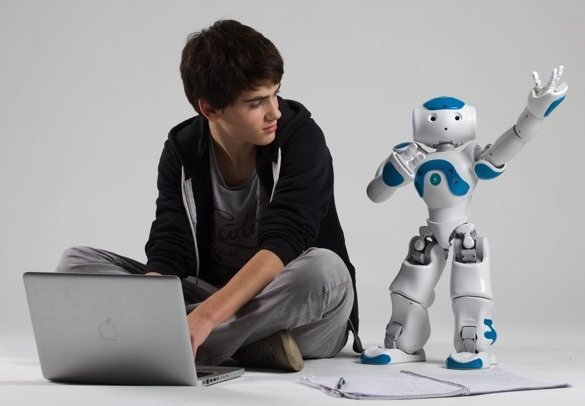
\includegraphics[width=15cm]{1.png}
\caption{Fully programmable NAO humanoid robot, \cite{naoPhoto1}}\label{naoRobot}
\end{figure}

\clearpage
\cleardoublepage

% CAPITOLUL 1
\section{Problem and Domain Analysis}
\phantomsection
\subsection{Problem definition}
    It is important to understand how to enable NAO to sort a set of objects. The task NAO has in front of him is similar to a task for a human to sort his socks or kitchen's cutlery. Humans put forks to forks, spoons to spoons and knives to knives. They group socks by their color. Thus humans find common traits and features in the given set of objects. A human is able to group objects even if he has never saw them before. He detects the characteristics of the objects using his sensors. NAO also should be able to group objects which are not in his data base. He should identify the objects, detect the common features and group them together. The images acquired by NAO's camera serve as the input. The change of the physical position of objects so that they are grouped together represents the desired output. The problem is to perform this transition.
           
            An input image is similar to any other picture taken by a camera. It has no additional clues nor information regarding the objects within it. No other sensors might give information to robot about objects in front of him. Robot receives a matrix of pixels. As robot does not see any object he does not feel how distant those are. An interesting subproblem is the distance determination to an object. Moreover, to group objects NAO takes into account only the visible features given a static representation of objects. The SDK that runs on robot does not provide the ready to use functionality for object identification or object grasping.
\subsection{Domain analysis}
    \subsubsection{Divide Et Impera}
        The task can be divided into three parts: object detection, object clustering and object movement.
        % \begin{enumerate}[topsep=5pt, partopsep=0pt,itemsep=3pt,parsep=1pt, itemindent=1cm]
        %     \item Object detection;
        %     \item Object clustering;
        %     \item Object movement.
        % \end{enumerate}
        The first part is the detection of objects from a given picture. Each object is described by a set of features. In order to detect their features, there is a need to extract all data related to  an object. Given that only the static image of the objects altogether is taken into account, the extraction of data is nothing else but the extraction of the sub image of each object. Here it is necessary to make the distinction between object recognition and object detection. The recognition deals with the task of identifying an object or a sub image which is already known, present in the data base. The system first receives a labeled image, then tries to label images with exactly the same structure. Object detection has the goal to identify instances of a certain class. For example, face recognition would say if the given input image contains John's face or not, while face detection for a given image would answer if there is any face in the picture. 

        The second part has to group detected objects into some logical groups. A group is logical when the objects within it are similar in a set of ways. These objects can be compared between them by comparing their features. This project deals with object clustering rather than with object classification. In Machine Learning context, a classification is the assignment of a class for a new object, having a set of predefined classes. Classification is represented by supervised machine learning algorithms, where the system has some labeled data first, on which it is trained, then when new data comes in, the system tries to figure out which label to put on it. Clustering, on the other hand, is the grouping of a set of objects if there is a relationship between them. Clustering is represented by unsupervised machine learning algorithms, where the system is given a set of unlabeled data, which might be divided into smaller sets, if any similarities are found. 

        The third part is the change of the position of the objects in such a way that these are all grouped in their groups. NAO should activate its motion module to first get closer to an object, position his hand above it, grasp it and move it to the corresponding place. 

A human uses different hints to conclude that there is an object in front of him. The details of this process are quite sophisticated. Humans can ``feel'' the distance, touch the surface, perform a way more complex visual analysis of the image they see, like taking into account the lights and shadows, reflection, etc. They remember the objects they have learned, so next time they recognize them. Humans also use the advantage of binocular vision, thus being able to “feel” the distance and create a 3-dimensional model of what they see.

Each of the above-discussed tasks can be divided into subtasks. In order to perform object detection a division into ``what is object'' and ``what is not'' is needed. What is not an object forms the background. It is clear that a lot of circumstances affect this concrete task. The nature of the background, the lighting conditions, the shadows and the eclipsing of one object by other should be taken into consideration. The clustering stage also might be performed in different ways. Robot might memorize the objects which he already learned, or he might pick them and look from different sides, as described in ``Active robot categorization'', \cite{categorization}. Objects might be big or small and they can be moved using one hand, both hands of even using legs. In order to define the scope of this project a set of assumptions is needed.

    \subsubsection{Assumptions}
        The task is going to be performed by NAO robot. His capabilities and limitations have a big impact over the way the task would be performed. Aldebaran Robotics provides a set of functionality enclosed into a SDK and additional helper software which may be used. A detailed analysis of NAO would be presented in the following sections, but it might be mentioned that NAO’s battery lasts about one and a half hour, his maximal walk speed is about 10cm/s. He has two cameras, whose angles of view do not intersect. There is no module for distance determination, though NAO can detect obstacles when he moves. His hand has only three fingers which makes it challenging to grasp objects. He cannot reach an object lying on the ground which is farther than 20cm from his feet, without first walking to it. His height is 573mm.

Because of these characteristics, it is assumed that only reasonably small objects would be used. These objects should be small enough so that the robot is capable of grasping them with one hand. Objects should be light enough and have a form which would permit to pick and lift them up. At the same time, because of camera quality limitations and NAO's hand construction objects should not be very small.There is no prior knowledge about the objects: NAO sees them for the first time when application runs for the first time. That also means that any object which passes previous requirements might be used. So the system should be able to group any object which is movable by NAO robot.

        The complexity of the image processing task imposes the assumption that the background should not complicate the main task. In other words, background should be easily distinguished from the objects, preferably being all of one color without additional drawings or different color zones. When the objects are located in front of the robot before the task, their view should not interfere with one another -- that is, objects should not overlap. There should be a reasonable number of objects, so that the task makes sense: at least a few objects, with different number of groups possible. Later an analysis of cases which are not included here might be done to see how robot performs. The objects which need to be sorted are positioned in front of NAO at the start of the experiment. All objects are in his view and there is no need for a search of them. 

The number of groups in which NAO should categorize the objects is not specified. The algorithm should deduce the number of clusters itself. Nevertheless, a possibility to intervene and coordinate robot’s actions should be introduced. For instance, the user can demand that NAO separate objects into exactly 4 groups. If the user does not, NAO decides that on his own.

    In order to connect remotely to NAO some network connectivity is needed (usually Wi-Fi). The surface on which NAO walks should be hard and smooth, the feet should have a good grip with the surface. No additional objects should come into play, such as some irregularities on the floor or a piece of furniture, or a door. The light and illumination conditions should be good enough, so that the images taken by camera are of high quality.

    \subsubsection{Existent solutions}
        Before starting the work an investigation of other theses and articles was done. In ``Vision-based grasping of objects'', \cite{visualGrasping} they analyze how NAO can grasp objects which he can reach with his hand without walking, using hand-eye coordination. While this approach is interesting, it is different from the need in this task, because in this case objects are on the floor and not in the immediate reach of hands. NAO would need first to approach to them, then pick them. In order to pick them, he needs to perform a complex movement in which hands would be able to reach the floor, which NAO cannot do while standing. In ``Object Learning with Natural Language'', \cite{objectLearning} is presented a neat solution for object detection, but there is just one object in front of NAO at once. Also, the main task they have there is object learning. The robot used there is quite different as well. ``Grab a Mug'', \cite{grabAMug} emphasizes the problem of grasping given the specifics of NAO’s hand, which has three fingers. It also shows the zones and distances were NAO can reach an object using his hands. ``Grasping Known Objects'', \cite{graspingKnownObjects} suggested a clear separation of tasks which are needed to be performed in order to make NAO grasp an object. 

        A similar task to the one of this thesis was performed in ``Active robot categorization'', \cite{categorization}. As here, NAO has to categorize the objects he is given. The significant difference is the fact that NAO has a prior database of learned objects. An interesting idea to make object identification more precise is to look at it from different points of view. As described, NAO takes the object in his hand, and rotates it to see it from front, top and side view. This work also points out a challenge in computer vision: ``There is a difficulty of handling rather small inter-class distances (cow vs. the horse in the middle) and high intra-class variability (the two horses)'', \cite{categorization}, as shown in figure \ref{horses}.
    \begin{figure}[ht!]
         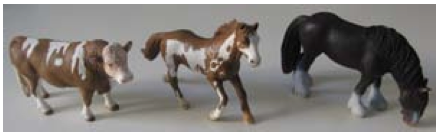
\includegraphics[width=10cm]{2.png} 
        \centering
        \caption{Small inter-class distances vs. high intra-class variability, \cite{categorization}}
        \label{horses}
    \end{figure}

    One of the most interesting for this project work is ``Object Grasping with the NAO'', \cite{objectGrasping}. It describes how using Machine Learning NAO can learn how to grasp objects. It gives a complete analysis and a detailed overview of three different approaches: Supervised Learning, Neural Networks and Reinforcement Learning. The thesis is totally concerned on grasping objects with two hands, which is not exactly what this project is about, but it is still very useful for analysis. 
A big part of the current problem deals with image processing. Object detection is also affected by shadows. ``Simple Shadow Removal'', \cite{shadowRemoval} describes a very efficient way to eliminate the shadow, which is also related to background subtraction. Even if these algorithms were not used here, they pointed out some useful ideas on object detection. 
    
    After these works have been analyzed it is clear that none of them does achieve the exact solution this thesis is concerned about. Many of them suggest how the solution might be achieved partially or indicate possible difficulties. Many ideas which were used in this thesis were inspired from the above-mentioned works.
\subsection{OpenCV Library}
    OpenCV (Open Source Computer Vision Library) is an open-source BSD-licensed library that includes several hundreds of computer vision algorithms. OpenCV is cross-platform. It focuses mainly on real-time image processing, but can be used also for statical images. Using the algorithms available in OpenCV it is easy to perform object detection, shadow and background removal, image processing and other things. There is even a machine learning module available. Since version 1.14, NAOqi SDK supports OpenCV for both compilation and cross-compilation. OpenCV has a modular structure, which means that the package includes several shared or static libraries. The following modules are used in this thesis:
    \begin{enumerate}[topsep=3pt, partopsep=0pt,itemsep=0pt,parsep=1pt]
        \item \verb|core|;
        \item \verb|imgproc|;
        \item \verb|video|;
        \item \verb|ml|;
        \item \verb|highgui|.
    \end{enumerate}

    The \verb|core| is a compact module defining basic data structures, including the dense multi-dimensional array \verb|Mat| and basic functions used by all other modules. The module \verb|imgproc| is an image processing module that includes linear and non-linear image filtering, geometrical image transformations (resize, affine and perspective warping, generic table-based remapping), color space conversion, histograms and so on. The \verb|video| module is a video analysis module that includes motion estimation, background subtraction and object tracking algorithms. The \verb|ml| module is the machine learning module which includes various algorithms implemented: neural networks, SVM, boosting, KNN, and others. The \verb|highgui| module is an easy-to-use interface for image, video codecs and simple UI capabilities, \cite{opencv}. As later would be described OpenCV is also providing the partial clustering functionality. The K-means clustering algorithm proved to be both efficient and satisfactory for project's needs. Shadow removal, background subtraction, finding of contours are the main tools used from OpenCV.
\subsection{NAO Robot}
    \subsubsection{Hardware Overview}
        NAO is a fully programmable humanoid robot. It is half-a-meter high and weights about 5 kilos. It is developed by Aldebaran Robotics. It comes with a suite of useful applications and a SDK available in 8 programming languages, \cite{naoDocumentation}.
        This hardware overview presents only the information relevant to this project. NAO H25 model of robot has a set of joints each of them powered by a motor. Each of these joints has a range of rotation. Robot’s CPU is Intel ATOM Z530 with one core, 32-bit architecture with clock speed 1.6GHZ. The motherboard has 1GB of RAM, 2GB of flash memory and also a MICRO SDHC for 8GB. It has two loudspeakers located in its ears. It has 4 microphones located in front, in the back, on the right and on the left side of his head. The two cameras are positioned on the front of the head, on a vertical line as presented in the figure \ref{H25model}. Cameras has 4 possible resolutions: 160x120, 320x240, 640x480 and 1280x960 (pixels). Each camera has a 47.64 degree vertical angle of view and 60.97 degree lateral angle of view, \cite{naoDocumentation}. 
        % The interesting joints for this task are the head and hand joints. 

        \begin{figure}[b!]
             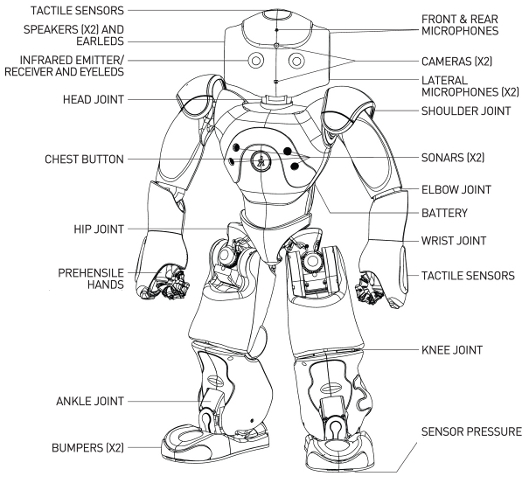
\includegraphics[scale=0.8]{3.png}
            \centering
            \caption{NAO H25 model components, \cite{naoDocumentation}}
            \label{H25model}
        \end{figure}
      \begin{figure}[b]
        \centering
        \subfloat[ Lateral view]
         {
         \label{background}
          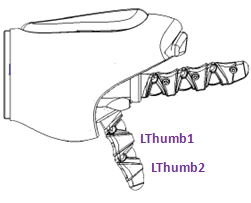
\includegraphics[width=0.35\linewidth]{4-1.png}
         }
        \hfil 
        \subfloat[ Front view]
         {
          \label{objects}
          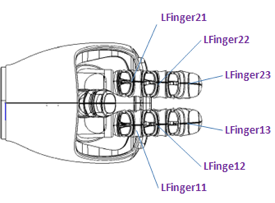
\includegraphics[width=0.45\linewidth]{4-2.png} 
         }
        \caption{NAO's left hand joints, \cite{naoDocumentation}}
        \label{NaoleftHand}
      \end{figure}
      %   \begin{figure}[ht!]
      %        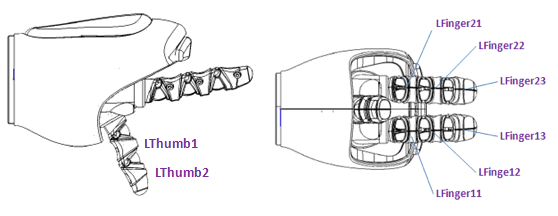
\includegraphics[scale=0.75]{4.png} 
      %       \centering
      %       \caption{NAO's left hand joints, \cite{naoDocumentation}}
      %       \label{NaoleftHand}
      %   \end{figure}
    \subsubsection{Software Overview}
        There are a set of applications and utilities provided by Aldebaran Robotics to help work with NAO. First of all, there is a complete SDK, original in C++, but also available for 7 other programming languages with some limitations regarding the functionality. The SDK is cross-platform, although there were problems to build a project on Mac OS X. There is a command line tool called \verb|qiBuild| aimed to manage the build process of a C++ project. It solves the dependencies and supports cross-compilation. A detailed description of the SDK would be given in a later chapter.

        The second software which makes testing of some basic things easy on NAO is Choregraphe. Choregraphe is a visual and behavioral programming IDE, available for all major platforms. It uses a simple GUI to build a program, connect to the robot by wireless and run it. There are a multitude of prebuilt behavior boxes which have inputs and outputs. These inputs and outputs might be connected to form a program execution flow. Each box has a Python script in the background, which might be edited. In a similar manner custom behaviors can be created. There is also a 3D model of the robot and its current state.
        \begin{figure}[t!]
             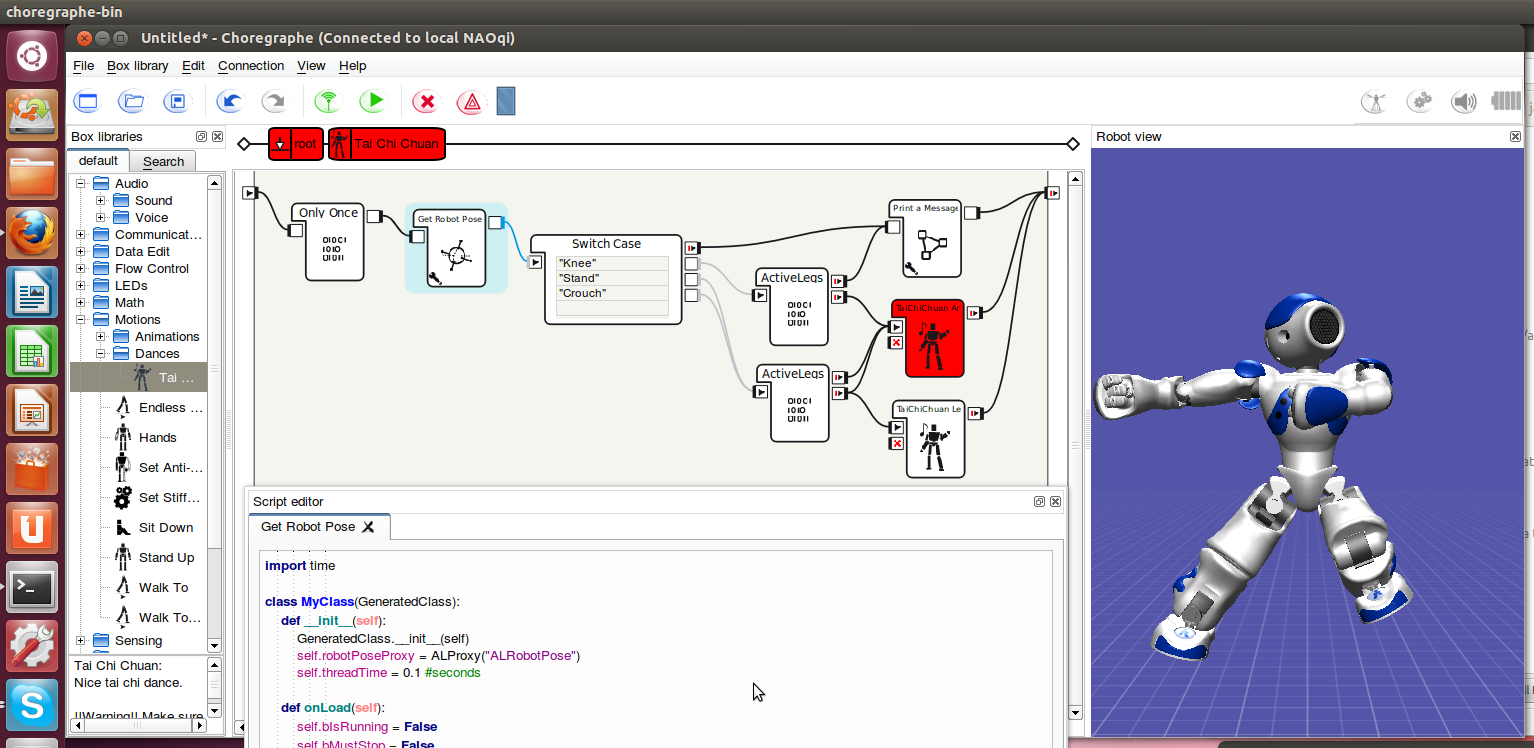
\includegraphics[width=0.95\textwidth]{5.png} 
            \centering
            \caption{Choregraphe visual programming tool}
            \label{choreographe}
        \end{figure}
        Choregraphe is a very useful way to get quickly introduced to the NAO. It is a simple way to see its possibilities.

         An important functionality to mention available in Choregraphe is the so called Animation Mode. In Animation Mode, robot becomes a puppet. The stiffness of his motors could be turned off, which make his body parts easily manipulable. While a user can turn for example his hands in way he likes, Choregraphe records the values to which motors should be actuated in order to perform such movement. Choregraphe later interpolates between two different positions robot was in so that the transition (which is the movement) from first stage to second happens smoothly. Later, such a motion might be exported as Python or C++ code.
% \newpage
        The next useful application which comes with NAO is Webots for NAO. Webots is a development environment used to model, program and simulate mobile robots, \cite{webots}. It is basically a virtual world were users can simulate their programs before running them on a real robot. Webots for NAO is a specific release of Webots, exclusively dedicated to the use of a simulated NAO. This program offers a safe place to test behaviors in advance. As any simulation it makes the testing cheaper and easier. It also offers the possibility to work remotely on a project without having an immediate need of a robot, requiring it only in the last instance.
        \begin{figure}[b!]
             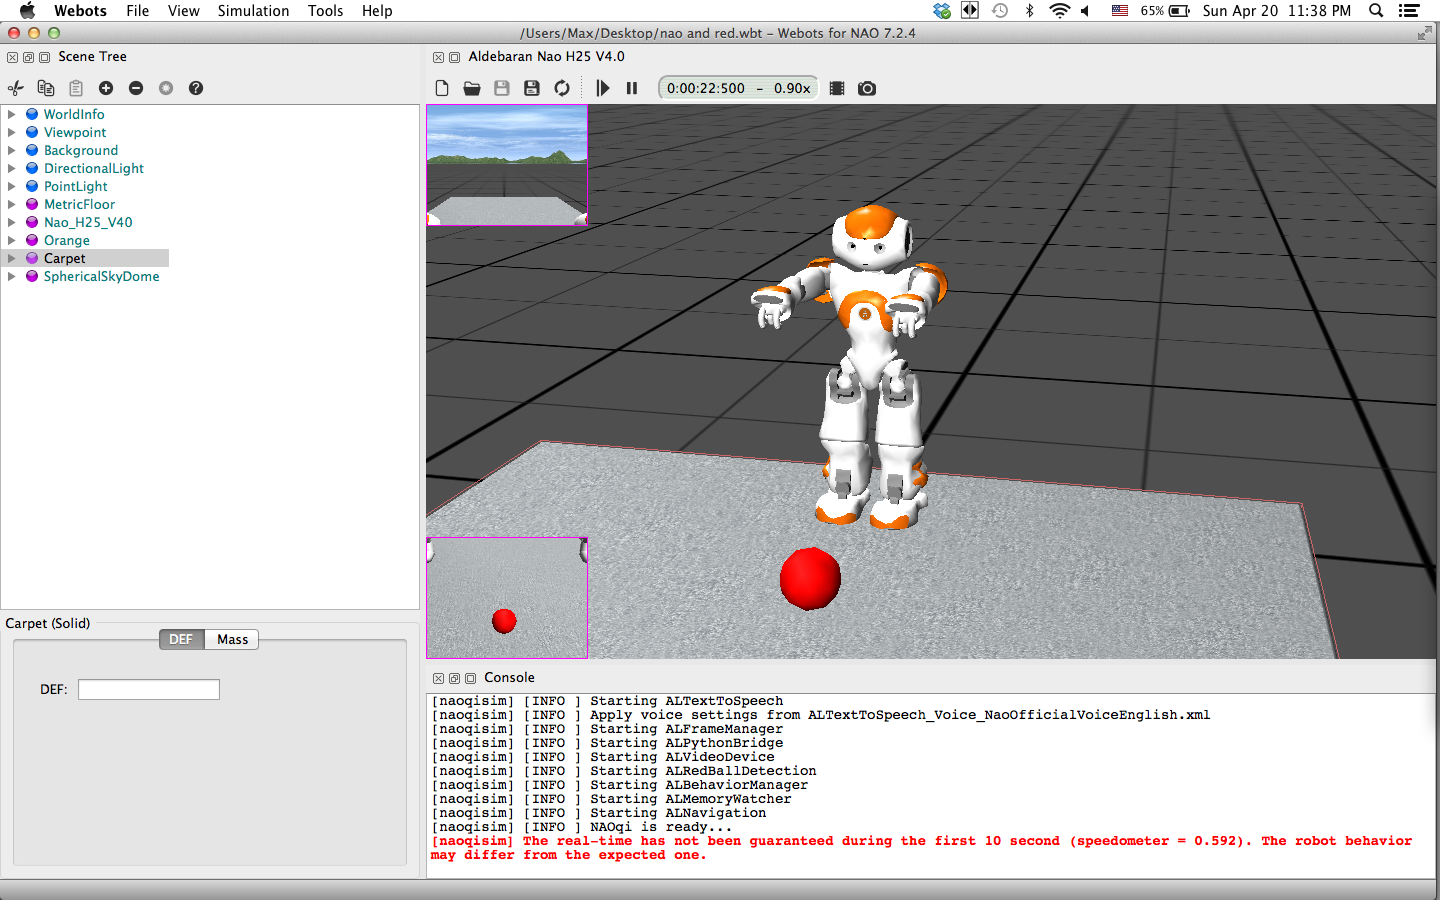
\includegraphics[width=0.95\textwidth]{6.png} 
            \centering
            \caption{Webots for NAO virtual simulator}
            \label{webots}
        \end{figure}
        Finally, there is a virtual image of the operating system running on robot which can be tested in a virtual machine. OpenNAO is a GNU/Linux distribution based on Gentoo. It’s an embedded GNU/Linux distribution specifically developed to fit the NAO robot needs. OpenNAO provides numbers of programs and libraries, among these, all the required one by \verb|NAOqi|, the piece of software giving life to the robot, \cite{naoDocumentation}.    

\subsection{Machine Learning}

    Machine learning is the science of getting computers to act without being explicitly programmed. In the past decade, machine learning has given people self-driving cars, practical speech recognition, effective web search, and a vastly improved understanding of the human genome. Machine learning is so pervasive today that everyone probably use it dozens of times a day without knowing it. Many researchers also think it is the best way to make progress to human-level AI, \cite{ml}.

    Machine learning deals with methods and algorithms which can learn or adapt to the environment. As mentioned previously, two biggest types of machine learning are Supervised and Unsupervised learning. Supervised or ``true'' learning is characterized by the fact that at the beginning an algorithm has a training set of data, on which the system is trained. The learning itself might be simply expressed as an optimization problem. The error function here represents the error between current output of the system and the desired one. The objective of the optimization is to minimize the error function. After the system is trained, it is ready to predict the outcome for the new data. 

    In unsupervised learning, there is no training set. Said differently, in supervised learning, the data is labeled -- for each input there is also the correct output given (a label), while in unsupervised learning the data is unlabeled -- there is only the input. Thus the goal of an unsupervised learning algorithm is to find hidden structure or relationship in unlabeled data. Unsupervised learning algorithms try to find similarities and common features in the input, thus creating some kind of output. 
        
    Clustering is an example of unsupervised learning. It is unsupervised learning, because there are no labels on the data. A set of input objects are given and these objects need to be grouped by similarities between them. Objects are similar, if the difference between them is small. The difference between objects can be expressed as the difference of same features of each object. Thus in the clustering part, each object is represented by its features. It is important to select the correct features, which really play the role of making objects similar or different. Today there are multiple toolboxes and machine learning libraries which offer a ready to use implementation of different algorithms. One example of such implementation is OpenCV built-in K-means clustering algorithm.  A detailed mathematical description of used learning algorithms would be given in the next chapter.
    % Later a custom method of clustering would be implemented and compared with the one which is built-in. The best of them would be used in this system.
          \begin{figure}[hb!]
        \centering
        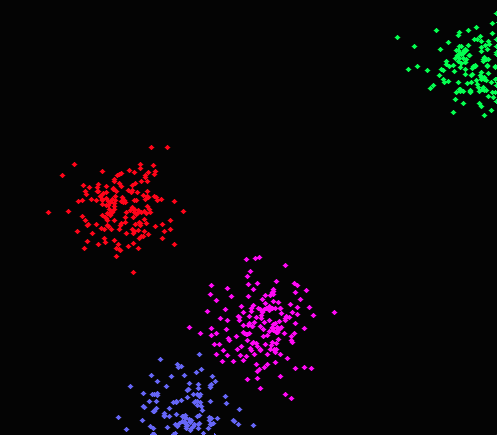
\includegraphics[width=0.4\textwidth]{11.png} 
        \caption{A clustering algorithm grouped the given points into 4 groups}
        \label{clusters}
      \end{figure}

\clearpage
\cleardoublepage

%CAPITOLUL2
\section{Mathematical Analysis}
\subsection{OpenCV algorithms}
    \subsubsection{Image representation}
      The core of the system would mainly deal with images. The structures which store images determine both the way the data is wrapped but also the approach for algorithms to take. All images are composed of pixels. An image is a matrix of them. In OpenCV, images can be of different color spaces. Different color spaces might require different number of channels (thus different amount of memory) to describe one pixel. The most important in this project are \verb|BGR| and \verb|GRAY| color spaces. \verb|BGR|, which is the default color format in OpenCV is often referred as RGB, but in OpenCV the order of bytes is reversed. \verb|GRAY| is a color space described by one channel which represents the intensity of the pixel, basically describing the transition from white to black. Thus each pixel is a set of numerical values, indicating the intensity of the corresponding channel. Using this representation, images can be added, subtracted or multiplied, between them or by a constant. All these operations are performed on matrices which stand behind the images. 
    \subsubsection{OpenCV built-in algorithms}

      As OpenCV is mostly a library of different algorithms, the following section describes OpenCV methods which were used in this thesis. As mentioned in the previous chapter, the first task is to identify the objects. This leads to the necessity of shadow elimination and background subtraction. Both of these algorithms are implemented in \verb|BackgroundSubtractorMOG2| class from OpenCV. The class implements the updated Gaussian mixture model background subtraction described in ``Gaussian mixture model and Density Estimation for background subtraction'', \cite{zivkovic},  \cite{heijden}. The code is very fast and performs also shadow detection. The shadow is detected if the pixel is a darker version of the background. A threshold defines how much darker the shadow can be, \cite{prati}. Basically, this algorithm is used to determine the background from a video, where many frames are present. It works, though, with only two frames as well: the first frame represents the clear background and the second depicts the objects. In the way this algorithm works, it is very similar to the direct subtraction of these two images: the same pixels would have similar numerical values and their subtraction would result in zero -- giving a black color for the mask. Other pixels, where objects appeared, would have the numerical value different from zero; using a specific threshold they can be recolored to white color, thus resulting into a corresponding mask.

      \begin{figure}[t]
        \centering
        \subfloat[ Background image]
         {
         \label{background}
          
\includegraphics[width=0.45\linewidth]{7-1.jpg}
         }
        \hfil 
        \subfloat[ Image with objects]
         {
          \label{objects}
          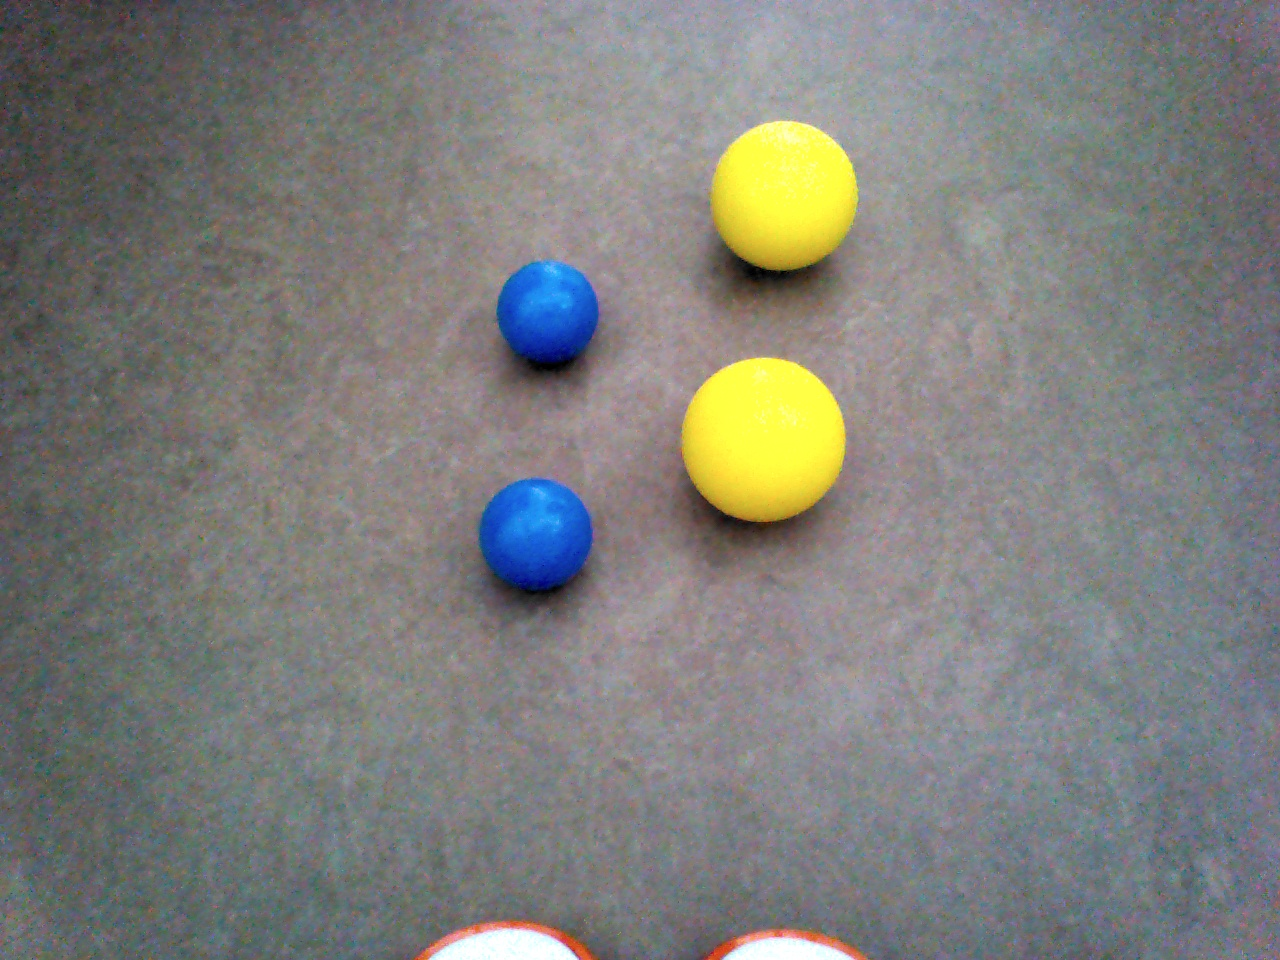
\includegraphics[width=0.45\linewidth]{7-2.jpg} 
         }
        \caption{Initial images}
        \label{backgroundAndObjects}
      \end{figure}

      As depicted in figure \ref{backgroundAndObjects}, there are two images. Remark the fact that in the background image (left one), at the right limit of the image there is a black spot, which disappears in the next image. This would affect the subtraction in figure \ref{mask}.
      \begin{figure}[t]
        \centering
        \subfloat[ Mask with shadow]
         {
         \label{withShadow}
          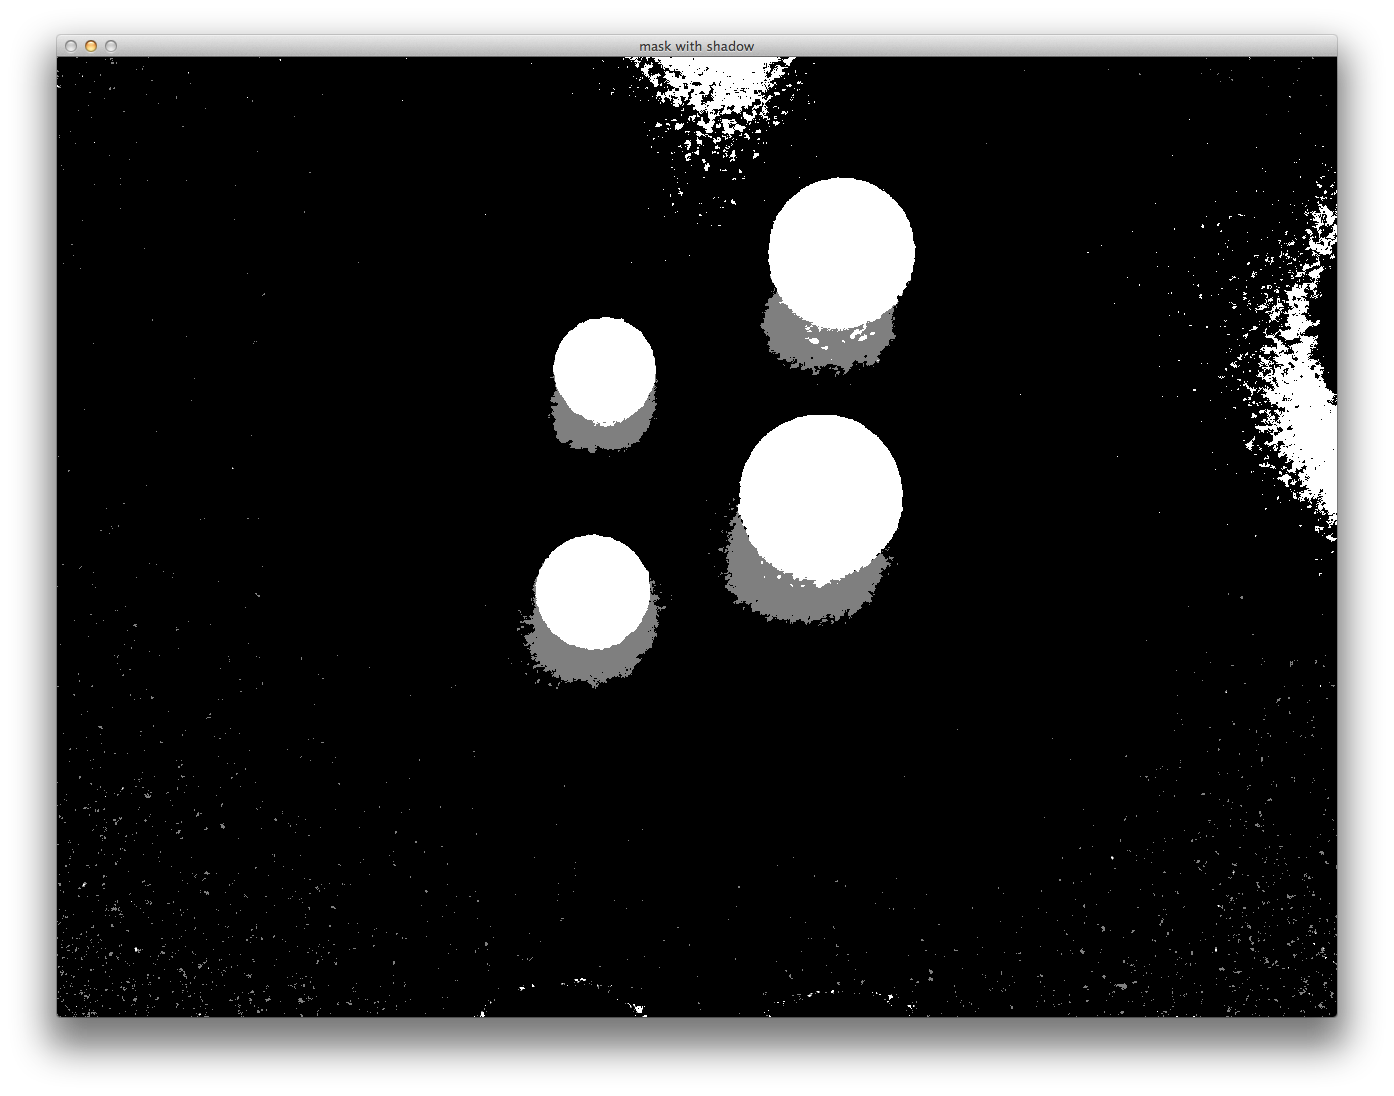
\includegraphics[width=0.45\linewidth]{8-1.png}
         }
        \hfil 
        \subfloat[ Mask without shadow]
         {
          \label{withoutShadow}
          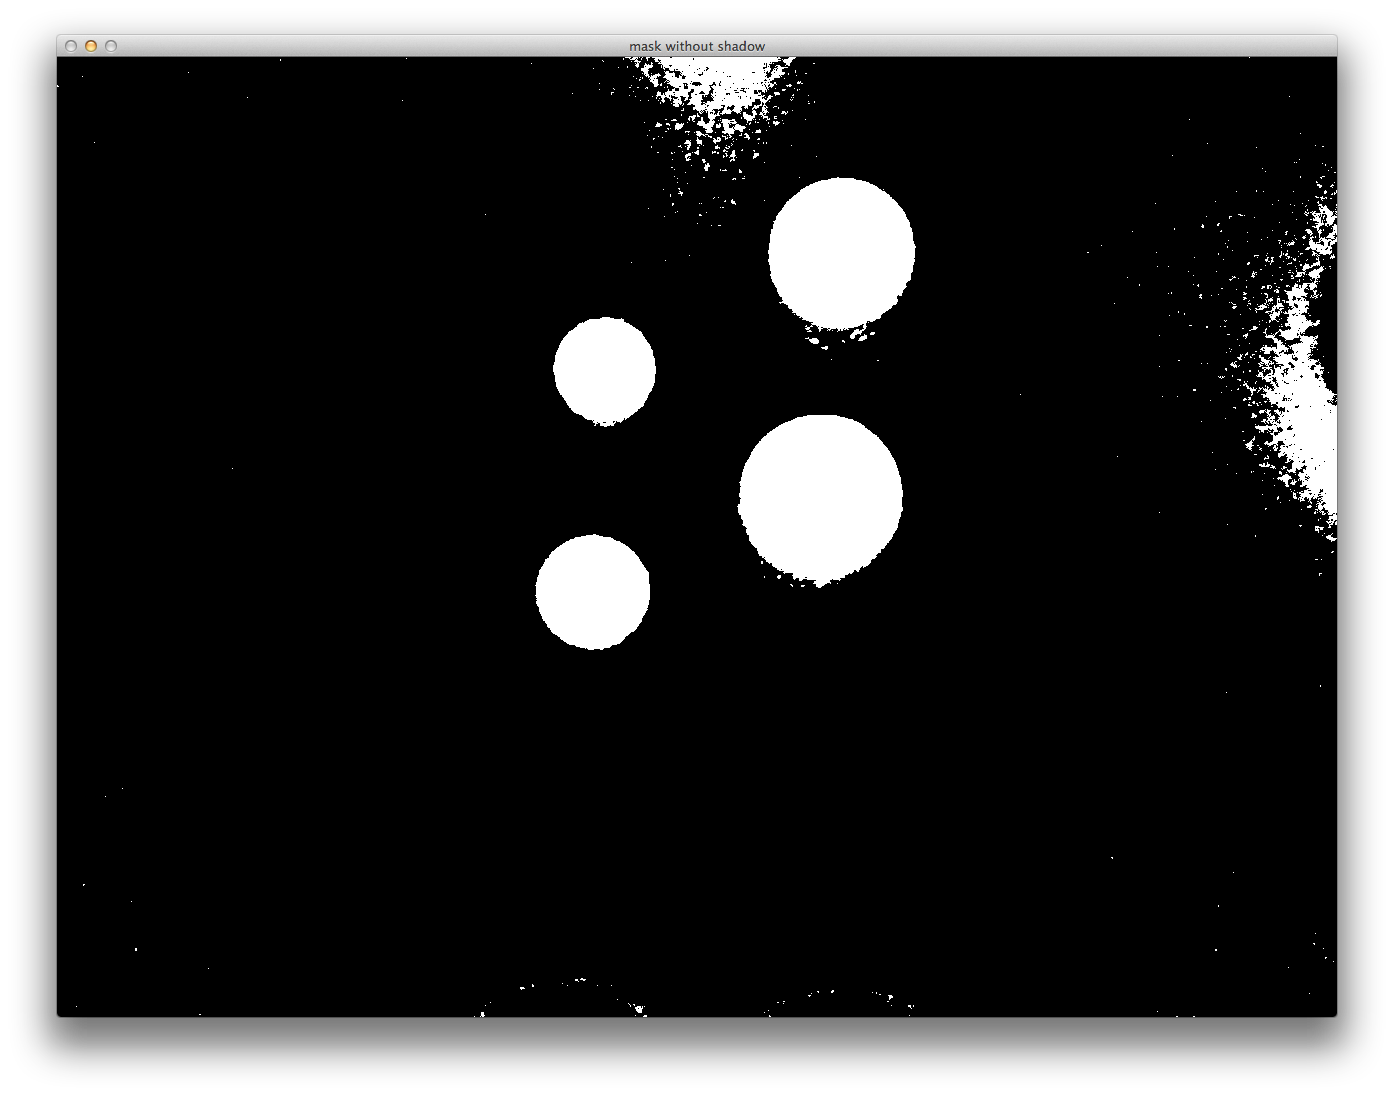
\includegraphics[width=0.45\linewidth]{8-2.png} 
         }
        \caption{Obtained mask after image processing}
        \label{mask}
      \end{figure}
Another interesting function used from OpenCV is the color space conversion. More precisely, there was a need for conversion from \verb|BGR| to \verb|GRAY| color space. \verb|BGR| has three channels while \verb|GRAY| has only one channel. The formula for this transformation, as presented in OpenCV documentation, \cite{opencv}, is:
\begin{equation}
        \label{conv}
          Y = 0.299\cdot R + 0.587\cdot G + 0.114\cdot B.
\end{equation}
      There are also other colorspace conversions which are not in the scope of this thesis. Smoothing or blurring is simple and frequently used image processing operation. To perform a smoothing operation a filter is applied over the image. The most common type of filters are linear, in which an output pixel’s value \(g(i,j)\) is determined as a weighted sum of input pixel values \(f(i+k,j+l)\):
\begin{equation}
        \label{wightedSum}
          g(i,j) = \sum_{k,l} f(i+k,j+l)h(k,l),
\end{equation}
      where \(h(k,l)\) is the so-called the kernel, which is nothing more than the coefficients of the filter. The utilized function smoothes an image using the following kernel: 
        \begin{eqnarray}
                \label{kernel}
          K = \frac{1}{k_{w}\cdot k_{h}} 
          \begin{bmatrix}
             1 & 1 & \cdots & 1 \\
             1 & 1 & \cdots & 1 \\
             \vdots  & \vdots  & \ddots & \vdots  \\
             1 & 1 & \cdots & 1 \\
           \end{bmatrix},
        \end{eqnarray}
where \( k_{w} \) is the kernel size width and \( k_{h} \) is the kernel size height.
      The most important in object detection are the functions for edge detection and creation of contours around the objects. These contours can be later enclosed in some rectangles, which can be cut from the initial image. Having as an input image the one as in the last figure, a threshold is specified which would depict the transition from black to white or vice-versa. The idea is based on a neighbor-pixels comparison. There are different approaches how to apply the threshold. For example, \verb|THRESH_BINARY| works in the following manner:
      \begin{equation}
       D(x,y) = \left\{ 
        \begin
          {array}{l l}
            V_{max} & \quad \text{if \(S(x,y)) > \nu_{T}\)}\\
            0 & \quad \text{otherwise},
        \end{array} 
        \right.
        \end{equation}
        where \( D \) is the destination matrix and \( S \) is the source matrix. \( V_{max}\) is the maximal value and \( \nu_{T}\) is the threshold. 
      Finally, in the obtained binary image the contours are found. The algorithm used in this function is presented in ``Topological Analysis of Binary Images'', \cite{suzuki}. The results of the images obtained in the last step would be as depicted in figure \ref{contours}.

      \begin{figure}[ht!]
        \centering
        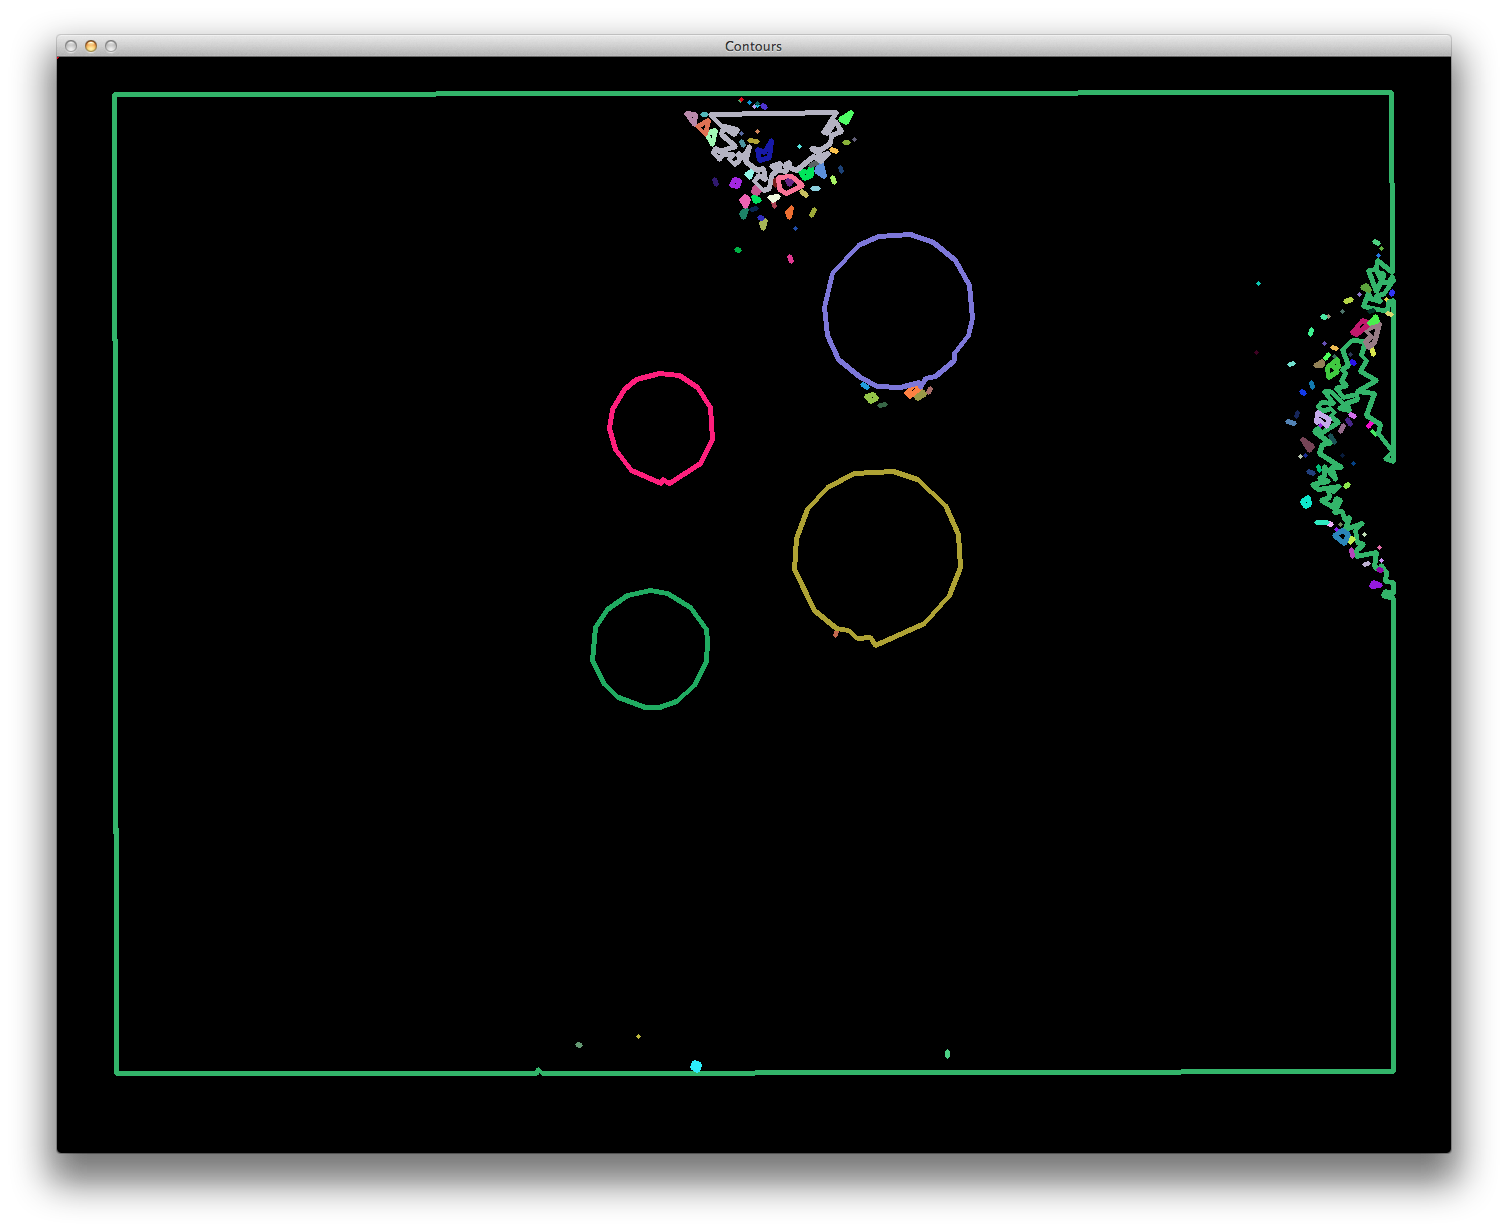
\includegraphics[width=0.8\linewidth]{9.png} 
        \caption{Contours of the detected objects and noise}
        \label{contours}
      \end{figure}

      As it is seen from the picture, there are multiple small contours which resulted because of the noise. Latter an easy way to tackle this problem will be presented. But before enclosing these figures into rectangles, a function for polygon approximation is used. This function approximates a curve or polygon with another curve/polygon with less vertices so that the distance between them is less or equal to the specified precision. It uses the Ramer-Douglas-Peucker algorithm. The simplified curve consists of a subset of the points that defined the original curve. The simplified idea would be to remove the points which are closer to the current line than some epsilon distance (initially the current line is the line formed by the first and last point). Finally, the program computes the bounding rect for each contour. As mentioned earlier, there are a lot of small contours which are useless in terms of objects the system needs to detect. It is easy to eliminate them by setting a lower bound for area the rectangle needs to have. In a similar fashion the very big rectangle which covers almost all picture is eliminated, by adding a upper bound on area. As a result the following rectangles are returned:

      \begin{figure}[t!]
        \centering
        \subfloat[ On the model image]
         {
         \label{black}
          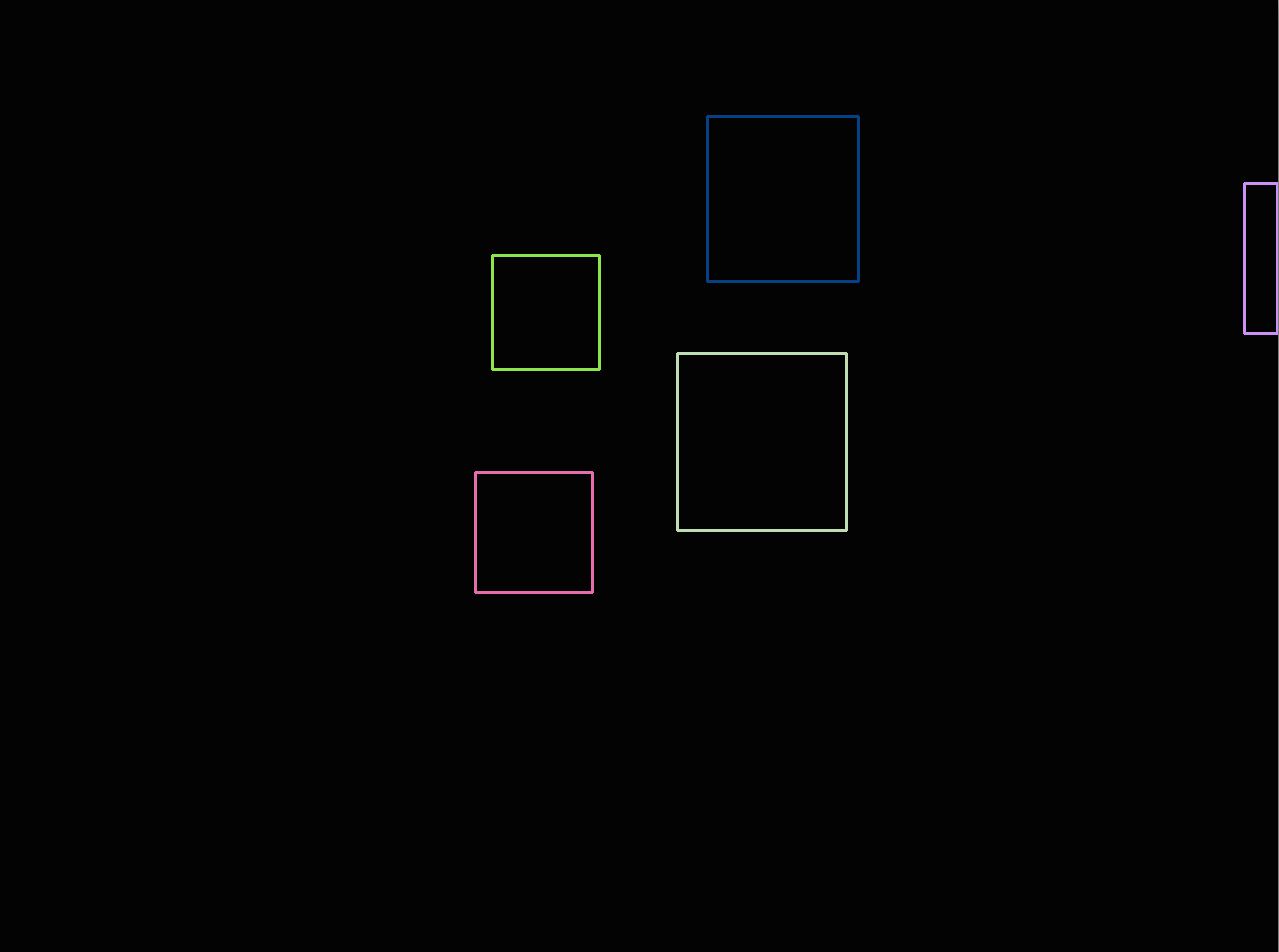
\includegraphics[width=0.45\linewidth]{10-1.png}
         }
        \hfil 
        \subfloat[ On the original image]
         {
          \label{onImage}
          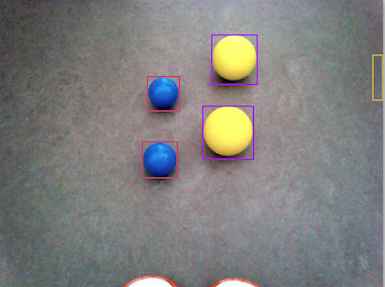
\includegraphics[width=0.45\linewidth]{10-2.png} 
         }
        \caption{Detected objects are enclosed into rectangles}
        \label{rectangles}
      \end{figure}

      Finally, the last algorithm from OpenCV which is used in this project is K-Means clustering algorithm. A more detailed description of it would follow in Machine Learning algorithms section. At first, a custom implementation of it was used. Later, for comparison reasons, the one implemented in OpenCV was added. While both perform quite well, the one from library gives a slightly better result and is optimized. The disadvantage of it was the fact that it does not determine by itself the number of clusters, thus a combination of OpenCV implementation of K-means together with custom determination of the number of clusters was used. 

The algorithm from library finds the centers of \( n\) clusters (where \( n\) is given) and groups input samples around the clusters. As an output an array of labels is returned, where element \( i\) contains a 0-based index for the sample stored in the \(i\)-th row of the matrix of samples. The function returns the compactness measure that is computed after every attempt:
        \begin{equation}
        \label{sumsum}
          \sum_{i} \| S_{i} - C_{L_{i}} \|^{2},
        \end{equation}
      where \( S_{i}\) is the vector of samples of \( i \) and \( C_{L_{i}} \) is the vector of centers which have the labels \(L_{i} \). The best (minimum) value is chosen and the corresponding labels and the compactness value are returned by the function, \cite{opencv}.


    \subsection{Distance computation}

      NAO has to reach and grasp the objects. In order to achieve that, he needs to know the location of the objects in space. The information which he has is the location of objects in the image and the position of the camera. Given that, it is possible to determine the distance between camera and objects. NAO's current position in space is also known. Concluding, the available information is enough to compute both the position of objects in space and the distance between them and NAO. 
      % In order to solve this problem, a selection of a coordinate system is needed.

      \subsubsection{NAO coordinate systems}

        NAO deals with three coordinate frames. For This project, two of them are important. The first one, denoted as \verb|FRAME_ROBOT|, has the origin in the average of the two feet positions projected around a vertical \(z\) axis. This space is useful, because the \(x\) axis is always forward, so provides a natural ego-centric reference. The second one is \verb|FRAME_WORLD|, which is a fixed origin that is never altered. It is left behind when NAO walks, and will be different in \(z\) rotation after NAO has turned. This space is useful for calculations which require an external, absolute frame of reference, \cite{naoDocumentation}. The figure \ref{axis} depicts how the axes in all coordinate spaces are oriented. 

        \begin{figure}[ht!]
        \centering
        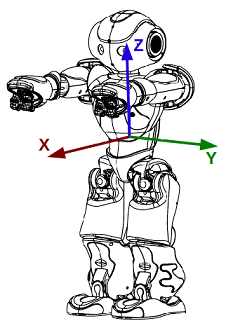
\includegraphics[width=4cm]{13.png} 
        \caption{Axes definition of the NAO's TORSO FRAME coordinate system, \cite{naoDocumentation}}
        \label{axis}
        \end{figure}

      An object in the image is bounded by a rectangle. Its position in image can be approximated to the center of that rectangle. The coordinates in the picture start in the top-left corner, \(x\) growing to the right, and \(y\) growing to the bottom of the image. 
A camera has horizontal and a vertical angle of view. The horizontal angle of view limits the distance to the left and right the camera can catch and the vertical angle of view limits the distance in the up and down directions which camera can catch. Translated to the NAO's coordinate systems axes, the vertical angle defines how far NAO can see on the NAO's \(x\) axis, horizontal angle -- on NAO's \(y\) axis. 
      If an object is higher in the image that means it is farther away in the forward direction. If an object is closer to the left side of the image, it should have a bigger value on the \(y\) coordinate of NAO's frame. 

      \begin{figure}[b!]
        \centering
        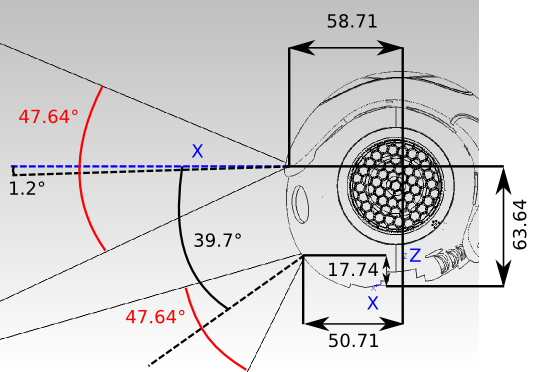
\includegraphics[width=0.75\linewidth]{14.png} 
        \caption{Angles and ranges of view of NAO's cameras, \cite{naoDocumentation}}
        \label{angles}
      \end{figure}

      NAO's camera position is available. The objects are located in the area close to NAO, so the bottom camera is used. This camera has a bigger angle of inclination with the NAO's \(x\) axe so that it ``looks down''. So this camera is used exclusively for all image acquisition. The position of the camera is described in \(x, y, z, wx, wy, wz\), where \(wx, wy, wz\) are the rotations around the corresponding axes. Thus the height of the camera and its inclination around \(y\) axis is available. Using simple Pythagorean theorem it can be computed how far the camera ``can see'' in the forward direction. But a camera has a vertical range of view, that is an angle of view which camera can percept. The current computed forward distance corresponds to the middle of this range of view. The lowest point in the image would correspond just to the start of the range of view, while the highest point -- to the end of it. Having the vertical angle at which the object lays it is possible to compute the forward distance toward it. The vertical range, as depicted in figure \ref{angles}, is \(47.64\) degrees.

      \subsubsection{Forward distance computation}

        The following formulas show how the object position is computed:
        \begin{equation}
          Y = \frac{N_{y} - O_{y}}{N_{y}},  0 < Y \leq 1,
        \end{equation}
        where \(Y\) represents the percentage of object's \(y\) coordinate in the image, \( N_{y}\) is \( y\) coordinate of NAO's position of the image and \( O_{y}\) is object's \( y\) coordinate in the image. If \(Y = 0\), it means the object is right at the bottom of the image; if \(Y = 1\), it means the object is right at the top of the image. \(N\) point is the position of NAO if he would be on the image. It was computed by solving the opposite problem to one which is explained now, but since there were more unknowns than equations, a heuristic approach was used. Basically, this position was approximated until the result was good enough. This position is a fixed position on the image before starting movement. The image has the size of \((1280,960) px\). NAO start position is \((640, 1070.43) px\). The position of the objects is calculated only once, before any movement. Next, the actual angle is computed (it is notated by \(\beta\)), which would be used to determine the forward distance. Angle \(\beta\) is the angle between the hypotenuse and the height of the camera and the remaining cathetus is the unknown forward distance.
        \begin{equation}
          \beta = 90 - \alpha - \frac{\gamma_{1}}{2} + Y\cdot \gamma_{1},
        \end{equation}
        where the \(\alpha\) is the angle of rotation of the camera around \(y\) axis retrieved from sensors before computation and \( \gamma_{1}\) denotes the range of vertical view. Finally, the forward distance \(F\) is:
        \begin{equation}
          F = h\cdot \tan \beta,
        \end{equation}
        where \(h\) is the camera height.

      \subsubsection{Lateral distance computation}
        Computing lateral distance, there is a need to take into acount the fact that farther is the point on the image, wider is the lateral distance. The horizontal range of view is increasing the distance on \(x\) axis as the look goes farther forward, as depicted in figure \ref{horizontalRange}.
        
        \begin{figure}[b!]
          \centering
          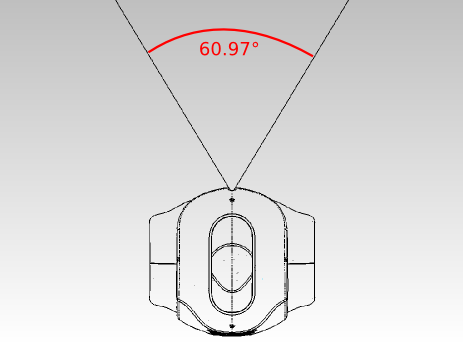
\includegraphics[width=0.6\linewidth]{15.png} 
          \caption{NAO's camera horizontal range of view, \cite{naoDocumentation}}
          \label{horizontalRange}
        \end{figure}

        In a similar way to \(Y\) coordinate, the \(X\) coordinate is expressed: 
        \begin{equation}
          X = \frac{O_{x} - \frac{I_{w}}{2} + N_{x}}{I_{w}},
        \end{equation}
          where \( I_{w}\) is the image width. If \(X = 0\) the object is on the left limit of the image; if \(X = 1\) the object is on the right limit of the image. Now, there are a two right triangles to deal with. The first one was already described -- it is the triangle formed by \(h\), \(F\) and \(\beta\) angle. Let's denote the hypotenuse of this triangle as \(P\). \(P\) represents the camera projection distance. The second triangle is formed by \(P\), \(L\) (lateral distance) and the angle \(\theta\), which is possible to compute. To compute distance \(P\) Pythagorean theorem is applied again:
          \begin{equation}
            P = \sqrt{F^2 + h^2}. 
          \end{equation}
           To compute angle \(\theta\) first angle \( \omega \) is calculated:
          \begin{equation}
        \omega = \frac{\gamma_{2}}{2},
          \end{equation}
          where \( \omega \) is the width angle and \(\gamma_{2}\) denotes the range of horizontal view. The angle \( \theta \) is:
          \begin{equation}
                \theta = -\omega + X\cdot \gamma_{2}.
          \end{equation}
          So the lateral distance would be:
          \begin{equation}
            L = h\cdot \tan \theta.
          \end{equation}
              Finally, to compute the object position, the above-calculated distances are added to the robot's current position. To verify how precise these results are, a series of tests were run. The image was divided into 12 zones and objects were placed in these zones. Their actual and computed positions were stored, then the error was computed. The results of measurements are presented in the table \ref{tab:items}. 
\begin{table}[t!]
\centering
\caption{Distance computation precision by NAO}
{
\renewcommand{\arraystretch}{2}
\begin{tabular}{ c|c|c|c|c|c|c }
\hline           
 Nr & \pbox{4cm}{Forward \\distance, m} &\pbox{5cm}{Lateral \\distance, m} &  \pbox{7cm}{Forward \\error, m} & \pbox{7cm}{Lateral \\error, m} &
  \pbox{7cm}{Forward \\error, \%} & \pbox{7cm}{Lateral \\error, \%} \\ \hline \hline
          1 & \( 0.4664 \) & \( -0.2181 \) & \( -0.0143 \) & \( 0.0357 \) & \( 1.2477 \) & \( 16.3769 \) \\ 
          2 & \( 0.4241 \) & \( -0.0500 \) & \( -0.0080 \) & \( 0.0046 \) & \( 0.6159 \) & \( 9.1024 \)  \\ 
          3 & \( 0.4241 \) & \( 0.1000 \) & \( -0.0026 \) & \( -0.0031 \) & \( 0.0760 \) & \( 3.0779 \) \\ 
          4 & \( 0.4509 \) & \( 0.2296 \) & \( -0.0206 \) & \( -0.0513 \) & \( 1.8835 \) & \( 22.3358 \) \\ 
          5 & \( 0.3000 \) & \( -0.1500 \) & \( 0.0054 \) & \( 0.0200 \) & \( 0.7200 \) & \( 13.3333 \) \\ 
          6 & \( 0.3500 \) & \( -0.0500 \) & \( 0.0019 \) & \( 0.0091 \) & \( 0.3728 \) & \( 18.2876 \) \\ 
          7 & \( 0.2900 \) & \( 0.0400 \) & \( 0.0032 \) & \( 0.0029 \) & \( 0.5032 \) & \( 7.2840 \) \\ 
          8 & \( 0.3100 \) & \( 0.1800 \) & \( 0.0009 \) & \( -0.0176 \) & \( 0.2693 \) & \( 9.7889 \) \\ 
          9 & \( 0.2500 \) & \( -0.1518 \) & \( 0.0034 \) & \( 0.0179 \) & \( 0.5200 \) & \( 11.7958 \) \\ 
          10 & \( 0.2400 \) & \( -0.0500 \) & \( 0.0063 \) & \( 0.0082 \) & \( 0.8072 \) & \( 16.4072 \) \\ 
          11 & \( 0.2300 \) & \( 0.0300 \) & \( 0.0034 \) & \( -0.0028 \) & \( 0.5216 \) & \( 9.2617 \) \\ 
          12 & \( 0.2400 \) & \( 0.1500 \) & \( -0.0011 \) & \( -0.0240 \) & \( 0.0711 \) & \( 15.9953 \) \\ \hline
          Mean & \( - \)  & \( - \) & \( 0.0060 \) & \( 0.0164 \) & \( 0.6340 \) & \( 12.7539 \) \\ \hline 
\end{tabular}
}
\label{tab:items}
\end{table}
      The forward distance computation is accurate enough. The average forward error is 0.6cm. The maximal forward error is almost 2cm. The lateral error, on the other hand, is bigger. Its mean error is 1.6cm. The maximal lateral error is almost 5cm. The forward and lateral distances themselves are quite small, bounded at 47cm and 23cm respectively. An error of 2-3cm is still acceptable in order for NAO to reach the destination and in the end grasp the object.


  \subsection{Machine learning algorithms}
    \subsubsection{K-means clustering}
          The materials presented in this section are integrally based on Machine Learning online course, \cite{ml}. Some of figures and formulas are taken from slides of this course, \cite{slides}.
Given a set of points, clustering is labeling each point with the group it belongs to. If all the points are similar, there might be just one cluster (group). In Machine Learning, the input points are denoted as \textbf{training set}. Clustering is used in Market segmentation, Social network analysis, Logistic of computer clusters and Astronomical data analysis, \cite{slides}. Mathematically, a training set is a vector of points:
      \begin{equation}
        [ x^{(1)}, x^{(2)}, \cdots, x^{(m)} ],
      \end{equation}
      where \( x^{(i)}\) denotes the training example \(i\). As a result, clustering should give a vector of labels:
      \begin{equation}
        [ y^{(1)}, y^{(2)}, \cdots, y^{(m)} ],
      \end{equation}
      where \( y^{(i)}\) represents the label for the training example \(i\). K-means algorithm itself takes the following input:
      \begin{gather}
        \nonumber
            K - \text{number of clusters} \\
            \nonumber
            [ x^{(1)}, x^{(2)}, \cdots, x^{(m)} ] - \text{training set} \\
            \nonumber
            x^{(i)} \in \mathbb{R}^n
      \end{gather}
      The \emph{K-Means algorithm} is presented below:
      \begin{algorithm}
        {Randomly initialize \(K\) cluster centroids $\mu_1, \mu_2, \cdots, \mu_K \in \mathbb{R}^n$}
        \begin{algorithmic}
          \Repeat 
          % \State {\emph{Cluster assignment step:}}
            \For{\( 1 \leq i \leq m \)}
              \State {\( c^{(i)} = \) index (from 1 to K) of cluster centroid closer to \( x^{(i)} \)} 
            \EndFor
          % \State {\emph{Centroid movement step:}}
            \For{\( 1 \leq k \leq K \)}
              \State {\( \mu_{k} = \) average (mean) of points assigned to cluster \( k \)} 
            \EndFor
          \Until{no changes}
        \end{algorithmic}
        \caption{K-Means algorithm}\label{alg:kmeans}
      \end{algorithm}
      \newline
      This algorithm consists of two steps. Each step is represented by a loop. The first \verb|for| loop is the \emph{Cluster assignment step}. In this step each point is assigned a label. This label represents the cluster which is the closest to the given point. The second step is represented by the second \verb|for| loop. This step is called \emph{Centroid movement step}. After the first step, each centroid has a number of points assigned to it. It recalculates the new position of the center (centroid) by computing the geometrical center of all the points. The process repeats until convergence -- the step after which label of points and the positions of centroids are unchanged.
        In figure \ref{pointsAndClusters} the result of a clustering is shown. 
              \begin{figure}[h!]
        \centering
        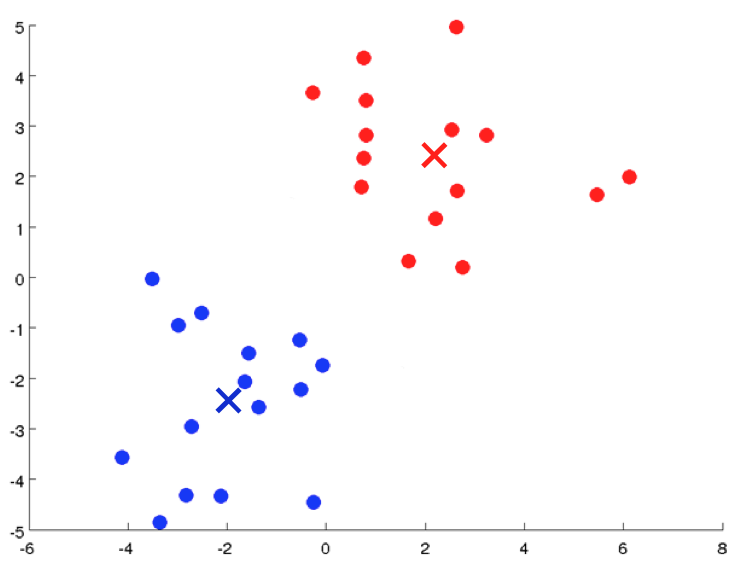
\includegraphics[width=0.45\linewidth]{16.png} 
        \caption{Points clustered into two clusters by K-means algorithm, \cite{slides}}
        \label{pointsAndClusters}
      \end{figure}

        \noindent The dots represent the points of the training set and the crosses are the centroids. The color shows the label of each point.
        In the start of the algorithm a random choice of centroids is performed. A different choice of centroids might lead to different results. This is usually not the desired result. In order to obtain the best result, the algorithm is run multiple times and the best outcome is chosen. The best outcome is the one which has the smallest error. A definition of the error function is needed. Given the following definitions:
        \begin{gather}
        \nonumber
          c^{(i)} - \text{index of cluster } (1, 2, ... , K) \text{ to which example } x^{(i)} \text{ is currently assigned}; \\
          \nonumber
          \mu_k - \text{cluster centroid } k  \text{ } (\mu_k \in \mathbb{R}^n); \\
          \nonumber
          \mu_{c^{(i)}} - \text{cluster centroid of cluster to which example } x^{(i)} \text{ has been assigned}.
        \end{gather}
        The error function is:
        \begin{equation}
          J(c^{(1)}, ..., c^{(m)}, \mu_1, ..., \mu_K) = \frac{1}{m}\sum_{i=1}^{m}\|x^{(i)} - \mu_{c^{(i)}}\|^2
        \end{equation}
        Basically the error function says that the error of clustering is the average of errors of each point, where the error of one point is the Euclidean distance between point and centroid. Having the error function, it is possible to define the optimization objective:
        \begin{equation}
        \begin{aligned}
        & \underset{ \mu_1, ..., \mu_K} { \underset{c^{(1)}, ..., c^{(m)}} {\text{min}} }
        & &  J(c^{(1)}, ..., c^{(m)}, \mu_1, ..., \mu_K)
        \end{aligned}
        \end{equation}
        Thus the goal is to minimize the error function. At the start of the algorithm a random initialization is performed. Random initialization consists of the following steps:
        \begin{enumerate}[topsep=5pt, partopsep=0pt,itemsep=3pt,parsep=1pt]
        \item Assure that \( K < m \) (number of clusters is less than the number of training examples);
        \item Randomly pick \( K \) training examples;
        \item Set \( \mu_1, ..., \mu_K \) equal to these \( K \) examples.
        \end{enumerate}


        Multiple runs of the algorithm are important because as previously mentioned, different choices of centroids lead to different results. This might happen because of local optimas of the optimization functions. In figure \ref{localOptimas} an example is shown how algorithm converged to the local optima. Thus the complete version of algorithm is presented in algorithm \ref{alg2}. In Machine Learning, the error function is usually called the \textbf{cost function}.
                \begin{figure}[h!]
          \centering
          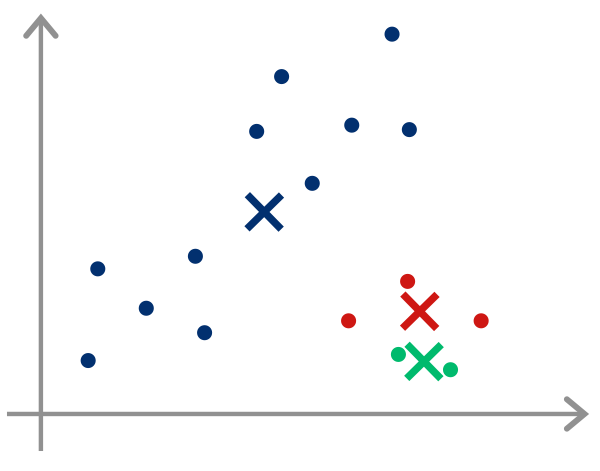
\includegraphics[width=5cm]{17.png} 
          \caption{Local optimas, \cite{slides}}
          \label{localOptimas}
        \end{figure}

      A custom implementation of K-means was done. Later it was compared with OpenCV built-in implementation. The second one was proven to be better, giving a smaller error. But the custom implementation could determine automatically the needed number of clusters. The technique used to determine the ``good'' number of clusters is called ``Elbow method''. In the end, the OpenCV implementation together with ``Elbow method'' were used:

        \begin{algorithm}
          \begin{algorithmic}
            \For{\( 1 \leq i \leq 100 \)} {\\}
              {Randomly initialize K-means \\}
              {Run K-means. Get \( c^{(1)}, ..., c^{(m)}, \mu_1, ..., \mu_K \).  \\}
              {Compute cost function(distortion) \( J(c^{(1)}, ..., c^{(m)}, \mu_1, ..., \mu_K) \).}
            \EndFor
            {Pick clustering that gave lowest cost \( J(c^{(1)}, ..., c^{(m)}, \mu_1, ..., \mu_K) \)}
        \end{algorithmic}
        \caption{K-Means algorithm with multiple runs}\label{alg2}
      \end{algorithm}



    \subsubsection{Elbow method}

      It is important to choose the right number of clusters -- \( K \). Sometimes even humans have different perspectives -- how would they group some objects -- it depends of their way of thinking. The desired effect is that when humans clearly see 4 different groups, so should the algorithm determine that there are 4 clusters. This number, \( K \), varies from 1 to \( m \), where \( m \) is the number of training examples. Indeed, there are two extremes: either all points go into one group, either each point is ``unique'', thus it cannot be grouped with others. The Elbow method offers a suggestion how this dilemma can be tackled. The idea is to look at the error. Given that the error is expressed in the distance of a point from the cluster, it is clear that if there are as many clusters as points, the error is zero -- each point is a cluster and each point is located in the same position as the centroid, distance being zero. So as the number of clusters increases, the error goes down. The interesting thing is that while the number of cluster increases and there are indeed enough groups for such a number, the error decreases very fast. As soon as \( K \) hits the optimal number, the error decreases at a slower speed. In figure \ref{elbow} a dependence of error to \( K \) is presented. As depicted, in the moment when \( K \) is optimal and the desired number of groups is hit, the slope of the line significantly changes, creating what is called ``the elbow'' (while the whole graph should be compared to an arm). 

      \begin{figure}[b!]
        \centering
        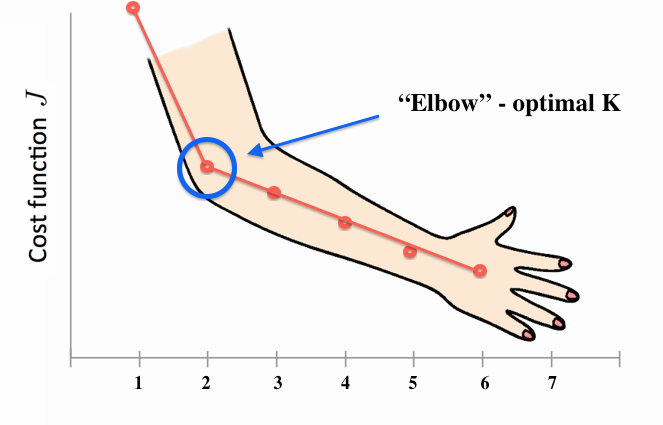
\includegraphics[width=0.6\linewidth]{18.png} 
        \caption{Elbow method illustrated}
        \label{elbow}
      \end{figure}


    \subsubsection{Going from points to images}

      It is easy to interpret all these notions on points. An adaptation if this algorithm to images is possible. The generalization lays in \textbf{features}. In Machine Learning, each training example is described by a set of features. For example a point has two features: \( x \) and \( y \) coordinates. Each training example \( x^{(i)} \) from the vector of examples is a vector itself -- a vector of features. Each feature is a simple number. The Euclidean distance between such training examples is the vector difference. But in order to make features uniform, they should be scaled and normalized. Let the training examples be some houses. Each house is characterized by a a set of features. A feature might be the number of bedrooms (that would be a one-digit number), or the size measured in \( m^2 \), which would be a number tens or hundreds time bigger. Features can have very different numerical values. While computing the distance, some of them might play a much higher role than others which is not the goal. Thus the transformations are performed: \textbf{feature scaling and normalization}.
      Feature scaling has the purpose to bring each \( x^{(i)}_j \) value (where \( x^{(i)}_j \) is the feature \( j \) of example \( x^{(i)} \)) into approximately \( [-1;1] \) range. This is done by simply dividing the current value to the maximal value of one feature across all examples. Feature normalization is the replacement of \( x^{(i)}_j \) with \( x^{(i)}_j - \mu_j \) to make features have approximately zero mean (where \( \mu_j \) is the mean value of feature \( j \) across all examples). 

      One of the most important roles in Machine Learning is played by feature selection. These values are the representative of the training examples. In this thesis, the training examples are the images of objects. The selected features should be good enough to mark the intraclass similarities and interclass differences. This is the list of selected features:
      \begin{enumerate}[topsep=0pt, partopsep=0pt,itemsep=0pt,parsep=1pt]
        \item image width;
        \item image height;
        \item mean red value of the image;
        \item mean blue value of the image;
        \item mean green value of the image;
        \item \( |width - height| \) -- how ``square'' is the image;
        \item image area.
      \end{enumerate}

      % \begin{figure}[hb!]
      %   \centering
      %   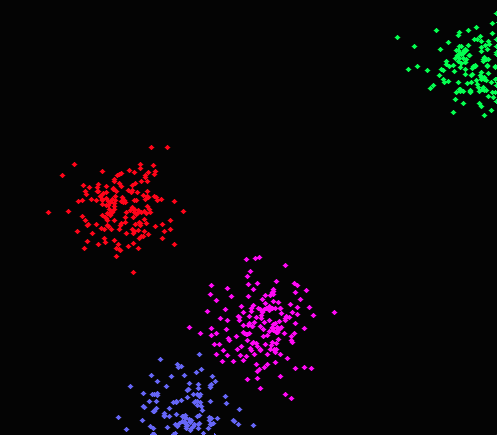
\includegraphics[width=0.525\linewidth]{11.png} 
      %   \caption{The result of OpenCV K-means clustering algorithm}
      %   \label{clusters}
      % \end{figure}

      \begin{figure}[hb!]
        \centering
        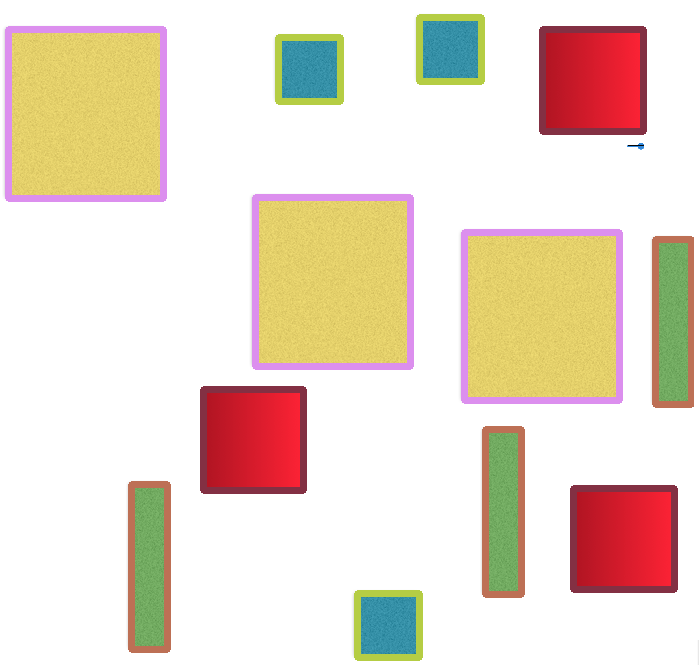
\includegraphics[width=0.35\linewidth]{19.png} 
        \caption{Example of clustering of simple shapes on a test image}
        \label{clusteringEx}
      \end{figure}




\clearpage
\cleardoublepage

%CAPITOLUL 3
\section{System Design and Implementation}
\phantomsection
\subsection{Requirements}
        \subsubsection{Functional requirements}
            The software should run on NAO. NAO should be able to sort a set of objects. That means NAO should be able to move. This also means that NAO should be able to ``see''. The last thing is that he should also be able to ``think'' in order to sort which object goes where. Now these very brief requirements would be expanded until the clear goals are defined. 
            Requirements:
            \begin{enumerate}[topsep=2pt, partopsep=0pt,itemsep=0pt,parsep=1pt]
                \item Move:
                    \begin{enumerate}[topsep=1pt, partopsep=0pt,itemsep=0pt,parsep=1pt]
                        \item walk;
                        \item stand up -- robot might start his activity sitting, so it is needed to stand him up;
                        \item sit down -- it is safe to leave the robot in the end in sitting state;
                        \item turn with the whole body to a relative degree;
                        \item take a custom position to grasp an object;
                        \item return to a standard position after grasping;
                        \item close hand -- grasp something;
                        \item open hand -- release something;
                        \item rise hand -- give the object to someone;
                        \item lower hand;
                        \item turn head to a relative direction -- look towards something.
                    \end{enumerate}
                \item See:
                    \begin{enumerate}[topsep=1pt, partopsep=0pt,itemsep=0pt,parsep=1pt]
                        \item take an image with the camera;
                    \end{enumerate}
                \item Think:
                    \begin{enumerate}[topsep=1pt, partopsep=0pt,itemsep=0pt,parsep=1pt]
                        \item compute distance -- ``feel'' how far is an object from the image;
                        \item detect objects:
                            \begin{itemize}[topsep=1pt, partopsep=0pt,itemsep=0pt,parsep=1pt]
                                \item[--] subtract background;
                                \item[--] eliminate shadow.
                            \end{itemize}
                        \item sort objects:
                            \begin{itemize}[topsep=1pt, partopsep=0pt,itemsep=0pt,parsep=1pt]
                                \item[--] extract features -- prepare for clustering;
                                \item[--] cluster objects -- group them.
                            \end{itemize}
                    \end{enumerate}
                \item Interact:
                    \begin{enumerate}[topsep=1pt, partopsep=0pt,itemsep=0pt,parsep=1pt]
                        \item receive commands -- speech commands;
                        \item execute commands -- react to them;
                        \item speak;
                        \item recognize speech;
                        \item detect audio source -- detect where is the speaker.
                    \end{enumerate}
            \end{enumerate}
        \subsubsection{Non-functional requirements}
            \noindent These requirements are dictated by circumstances or are implied by functional requirements. 
            \begin{enumerate}[topsep=2pt, partopsep=0pt,itemsep=0pt,parsep=1pt]
                \item The programming language required is C++ because this is the only one which can be executed locally on NAO;
                \item Project should be cross-platform: run both on Linux and Mac OS X;
                \item For better object detection take two pictures: one of plain background and the second one already with objects;
                \item Use the available libraries and SDK-s and their functionality;
                \item Use Qt Creator as IDE because this one is recommended and \verb|qibuild| can create projects for it;
                \item Build on Linux because cross-compilation feature is available only in Linux version of NAO SDK. So to build a project which would run on robot Linux is required;
                \item Store all images in OpenCV internal format, since this is the format received from the camera and good for all image processing algorithms.
            \end{enumerate}\itemsep0pt

\addtocontents{toc}{\protect\newpage}

    \subsection{Compilation process}
            NAO robot runs a Linux-like operating system. There are two ways to execute a program on NAO: \textbf{local execution and remote execution}. In the first case, all the code runs on NAO and this is the fastest possibility to retrieve data from \verb|ALMemory| module where all the values of sensors are stored. To deploy something on NAO, the code should be written in C++. Having your code on a PC or laptop, it is needed to build the project for a different machine -- for the robot. This action is called \textbf{cross-compilation}: compilation and creation of an executable for a platform other than the one on which compiler is running. Such a functionality is available only in the SDK for Linux operating system (though NAO SDK is available also for Mac OS X and Windows). Remote execution is running the executable on a different machine, while accessing robot functionality through network. This functionality is implemented with Proxy pattern in mind -- in code a proxy to a certain module is created, then the functionality of this module is used. This way is slower in terms of accessing NAO's modules but it has the advantages of using a more powerful processor, since the processor on robot is quite robust in terms of processing power. During this project, only remote execution was used.

            NAO SDK comes with a tool for building. It is similar to \verb|make|. It is called \verb|qibuild|. \verb|qibuild| manages dependences between projects and supports cross-compilation. Below are presented the needed commands to create and build a project. The following steps need to be performed:
            \begin{enumerate}[topsep=2pt, partopsep=0pt,itemsep=0pt,parsep=1pt]
                \item create a worktree: \verb|qibuild init|
                \item create a project: \verb|qibuild create foo|
                \item configure and make the project: \verb|qibuild configure -c mytoolchain foo|
                \item        \verb|qibuild make -c mytoolchain foo|
                \item to open a project in an IDE (for example, Qt Creator): \verb|qibuild open foo|
            \end{enumerate}


        \subsection{Object-oriented design}

        Object Oriented Programming is perhaps the most successful approach to software development. Moreover, the foundation on which this program should be build is written in OOP style as well, both NAO SDK and OpenCV. That is why such an approach would be used here. But before designing this system, there is need to explore the available SDK-s first. That way it would be clear what is already implemented and how this can be used in current project.

    \subsubsection{NAOqi API}

        NAOqi is the name of the main software that runs on the robot and controls it. The NAOqi Framework is the programming framework used to program NAO. It answers to common robotics needs including: parallelism, resources, synchronization, events. This framework allows homogeneous communication between different modules (motion, audio, video), homogeneous programming and homogeneous information sharing, \cite{naoDocumentation}. It runs on robot but also can be installed on a different machine to be run on a simulator. The NAOqi API is currently available in at least 8 languages. Apart from some minor language-specific differences, the API is mostly the same across all languages, allowing you to bring knowledge from one language to another. The C++ framework is the most complete framework. It is the only framework that lets you write real-time code, running at high speed on the robot (with loops of less that 10 ms, for instance).

    All the functionality of NAOqi is separated into modules. Each module is composed of concrete classes which implement the specific functionality. The modules are:
        \begin{enumerate}[topsep=5pt, partopsep=0pt,itemsep=3pt,parsep=1pt]
            \item Core -- NAOqi comes with a list of core modules that are always available. Every module comes with a list of default methods.
            \item Motion -- the \verb|ALMotion| module provides methods which make NAO move.
            \item Audio -- this represents the audio software components that run on robot.
            \item Vision -- for vision.
            \item Sensors -- deals with bumpers, tactile hands, tactile head and chest button. Also includes data from battery infrared sensors, sonars and laser.
            \item Trackers -- the Tracker modules allow you to make NAO track targets (a red ball or a face). The main goal of these modules is to establish a bridge between target detection and motion in order to make NAO keep in view the target in the middle of the camera.
            \item DCM -- Device Communication Manager, is a Hardware Abstraction Layer.
        \end{enumerate}
        Not all of these modules were used. Next the specific classes important for this project would be described and their functionality.
        \verb|ALError| is used to send exception. All NAOqi errors are based on exceptions. All user commands should be encapsulated in a try-catch block. Example of usage:
        \renewcommand{\thelstlisting}{\thesection.\arabic{lstlisting}}
        \lstinputlisting[language=C++, caption={Try-catch block in NAOqi}, label=list1]{../SrcCode/tryCatch.cpp}
\vspace{5mm}
        The module \verb|ALTextToSpeechProxy| is used to make NAO say something. As it can be observed, this and most of the following modules would have the postfix \verb|Proxy| which signifies the fact that this class acts like a proxy to a real speech module which runs on robot (while this module is used for remote execution). Example of usage:
        \lstinputlisting[language=C++, caption={Text-To-Speech functionality}, label=list2]{../SrcCode/tts.cpp}
\vspace{5mm}
        \verb|ALMotionProxy| is used for generic movements of any part of the robot's body, as well as for position retrieval. As a general pattern, all \verb|Proxy| classes take as an argument a \verb|std::string| which is the robot's IP, so the module could connect to the robot. Here's an example how to get the robot's position in space:
        \lstinputlisting[language=C++, caption={Getting robot's position}, label=list3]{../SrcCode/motion.cpp}
\vspace{5mm}
        \verb|ALRobotPostureProxy| is a class which implements the functionality of getting robot into one of the predefined postures. There are 8 predefined postures, like \verb|Stand| or \verb|Sit|. The method \verb|goToPosture| is the most important one, which takes care of other things as well:
        \lstinputlisting[language=C++, caption={Changing robot's posture}, label=list4]{../SrcCode/posture.cpp}
\vspace{5mm}
        \verb|ALNavigationProxy| implements safe walking. It subclasses \verb|ALMotionProxy|, using the generic movement in the back, but also checks for an obstacle thanks to the sensors. If there is an obstacle, the robot stops. 
        \lstinputlisting[language=C++, caption={Safe walking}, label=list5]{../SrcCode/walking.cpp}
\vspace{5mm}
        \verb|ALValue| is a generic wrapper of data in NAOqi. Numerous methods return the information stored in this form, or take it as a parameter.
        \verb|ALVideoDeviceProxy| is the accessor to the NAO's camera. To get an image remotely, one must first subscribe to the camera as a client, then ask for an image:
        \lstinputlisting[language=C++, caption={Getting images from camera remotely}, label=list6]{../SrcCode/getImage.cpp}
\vspace{5mm}
        \verb|ALMemoryProxy| is the class which gives the access to all the data from sensors and robot parts. The method \verb|getData| takes a string as an argument specifying which data to return. The next example shows how to retrieve data related to speech recognition of certain words:
        \lstinputlisting[language=C++, caption={Accessing NAO's memory}, label=list7]{../SrcCode/memory.cpp}
\vspace{5mm}
        But to start the speech recognition we need to first set some parameters and use the \\\verb|ALSpeechRecognitionProxy| class:
        \lstinputlisting[language=C++, caption={Speech recognition functionality}, label=list8]{../SrcCode/speech.cpp}
\vspace{5mm}
        Because NAO has 4 microphones, it can compute with some limited precision where the source of the sound is located. This functionality is built in \verb|ALAudioSourceLocalizationProxy| class.
        \lstinputlisting[language=C++, caption={Sound localization functionality}, label=list9]{../SrcCode/soundLocalization.cpp}
        \vspace{5mm}
        This is basically all the functionality of the robot which is needed for this project. Next, an analysis of OpenCV used methods and classes is presented.


    \subsubsection{OpenCV API}

        OpenCV was discussed in the previous chapter. This section briefly summarizes the used API. 
        The basic data structure used throughout the whole framework is \verb|cv::Mat|. In order to get access to it, there should be included \verb|opencv2/opencv.hpp| header file, but other OpenCV headers contain these primary definitions as well. A \verb|Mat| represents a matrix. It offers the implementation of basic matrix operations, both with other matrices and with scalar numbers as well. It is the structure used to store data of all the images. Besides \verb|Mat|, \verb|cv::Point2d| is used for representation of points and pairs of numbers. The structure \verb|cv::Rect| was used to represent a bounding rectange of a subimage and in object detection. To read an image form the file system call: 

        % the function \verb|cv::imread| is called with first parameter a string with file location and second parameter a constant indicating in which format should the file be read: 

         % The core functionality of OpenCV is given in \verb|opencv2/core/core.hpp| file.

        \verb|mat = cv::imread( BACKGROUND_IMAGE, CV_LOAD_IMAGE_COLOR );|

         \noindent While performing the object detection the following modules are used: 
        \begin{enumerate}[topsep=5pt, partopsep=0pt,itemsep=3pt,parsep=1pt]
            \item image processing module, defined in     \verb|opencv2/imgproc/imgproc.hpp|;
            \item GUI model (for windows and outputs),
            defined in \verb|opencv2/highgui/highgui.hpp|;
            \item the background segmentation algorithm,
            defined in \verb|opencv2/video/background_segm.hpp|;
        \end{enumerate}\itemsep0pt

        To show an image in a window the following functions would be used:
        \lstinputlisting[language=C++, caption={Show image functionality}, label=list10]{../SrcCode/showImage.cpp}
\vspace{5mm}
        To subtract the background, first a matrix mask is defined. It will contain the differences between background and foreground. Then an instance of \verb|BackgroundSubtractorMOG2| class is created and some parameters are adjusted: After that, the images of background and foreground are fetched to the instance and the mask is received:
        \lstinputlisting[language=C++, caption={Background subtraction}, label=list11]{../SrcCode/subtraction.cpp}
\vspace{5mm}
        The access of a pixel itself in a gray-color image is done in the following way:

        \verb|mask.at<uchar>(i,j) = 0;| 

        \noindent where \( i, j \) represent the row and column in the matrix. There is just one value -- the intensity. To access a pixel of a RGB image a similar procedure is done:

         \verb|cv::Vec3b pixel = mat.at<cv::Vec3b>(x,y);| 

         \noindent but here one pixel is a 3-dimensional vector. To convert an image from RBG to  gray scale it is possible to call:

        \verb|cvtColor( recolored_src, src_gray, CV_BGR2GRAY );|

        \noindent To blur an image simply call: 

        \verb|blur(src_gray, src_gray, cv::Size(3,3) );| 

        \noindent To detect a threshold the following code is executed:

        \verb|threshold( gray, threshold_output, i, 255, cv::THRESH_BINARY );| 

        \noindent To find contours: 
        \lstinputlisting[language=C++, caption={Finding contours}, label=list12]{../SrcCode/contours.cpp}
\vspace{5mm}
       Next the contours can be approximated to polynomials:

        \verb|approxPolyDP( cv::Mat(contours[i]), contours_poly[i], 3, true );| 
       
         \noindent and a polynomial might be bounded by a rectangle:

         \verb|boundingRect( cv::Mat(contours_poly[i]) );|

        \noindent To use the OpenCV built-in K-means clustering algorithm:
        \lstinputlisting[language=C++, caption={K-means clustering}, label=list13]{../SrcCode/clustering.cpp}

    \subsubsection{Objects and classes}

        Before starting the design of the system and defining the classes it is preferable to first look which objects there are, then group them into classes. There is a robot. So there should be a class \verb|NAO|. There are real objects, like a duck or a ball or a chess figure; so there should be a class which reassembles an object. On NAO, there is the camera, but when the project runs on Mac OS X the images are retrieved from the file system. Thus there should be a class which generalizes the functionality, let's say \verb|ImageFetcher|. The project deals with images, there is an object which can cluster, one which can move, one which can compute the distance, other which can speak and listen. All these are integrated in NAO. So we would have some kind of composition. Many of the above responsibilities can be performed by a \verb|Head|. But a class should have only one responsibility. So the head would unify all these processes. Going out from the rule of thumb that one class should have only one responsibility, the following classes were defined:

        \begin{enumerate}[topsep=3pt, partopsep=0pt,itemsep=1pt,parsep=1pt]
            \item \verb|Speech|;
            \item \verb|CustomMoves|, \verb|Locomotion|, \verb|SpaceOrientation| -- for locomotion;
            \item \verb|Image|, \verb|Object|, \verb|ObjectDetector|;
            \item \verb|AbstractImageFetcher|, \verb|Camera|, \verb|ImageFetcherOnOSX|;
            \item \verb|AbstractClusterAlgorithm|, \verb|KMeansClusterAlgorithm|;
            \item \verb|Head|, \verb|NAO|, \verb|Factory| (implements the corresponding design pattern).
        \end{enumerate}\itemsep0pt


    \subsubsection{Relationships between classes}
        The following diagrams present the structure of the system. They present the classes from which this system is composed and the relationship between them. They also show the dependencies. The use case diagrams of the system can be found in the appendix A.    
        In figure \ref{image} The \verb|Image| class is just a wrapper of OpenCV \verb|cv::Mat| class with additional helper methods. The image of objects or background is obtained from some \verb|AbstractImageFetcher| -- is it a camera, on robot or just some pictures from the filesystem on Mac OS X. All the classes which access NAO SDK modules need to know the robot's IP. This one is given as argument to the constructor, as a string (see \verb|Camera| class). To get an image from the robot using the proxy the corresponding SDK calls are performed. Because the SDK is available only on Linux, a platform check is performed: \verb|#ifdef __linux__| then the SDK is used. The center of the image is not contained in an attribute, but is computed every time its getter is called from \verb|boundingRect|. Each class has also the copy constructor implemented and assignment operator overloaded. Besides that, the stream operator is overloaded as well. The stream operator ``streams'' all the members of the corresponding class. From the diagram we can see that the class \verb|Image| has private attributes \verb|matrix| and \verb|boundingRect| and it also knows about \verb|cv::Point2d|.
         

        \begin{figure}[h!]
            \centering
            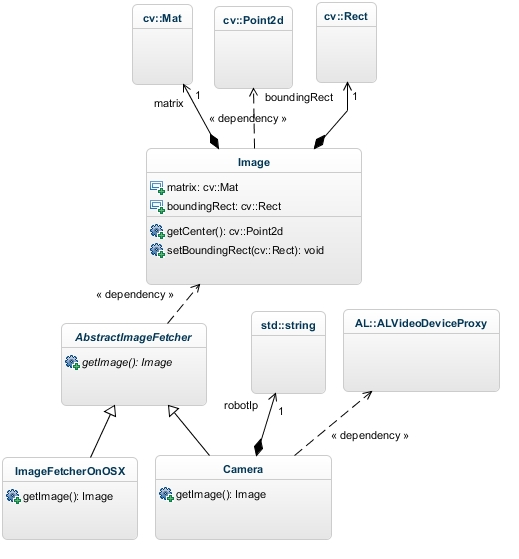
\includegraphics[scale=0.9]{21.eps} 
            \caption{Image Fetcher classes}
            \label{image}
        \end{figure}
% \newpage
        In figure \ref{detector} the \verb|Object| class is represented by an image. It has a position in space and in the scope of this project it has a property called \verb|group|, which is the label received after clustering. The class \verb|ObjectDetector| has just one public method: \verb|detectObjectsFromImage()|. All the intermediary steps of detection should be implemented in private methods. The detection algorithm implemented in \verb|ObjectDetector| class is presented in figure \ref{activity1}. This algorithm is simple and it contains a uniform flow of steps. Behind the private methods shown in the detector, there are operations like checking if a rectangle is inside another rectangle or recoloring a set of pixels to the color of background. Some constants of minimal and maximal area of acceptable objects are also defined in the header file. The class \verb|BoundingRect| has properties like top left corner and bottom right one, rectangle width and height. In the start, the detection was implemented in such a way that the objects would be extracted from just one image. It took into account notable differences between the colors on neighbor pixels, but such an implementation would never work on a background like chess board. It proved to be erroneous, because it is difficult to make sense what is the background just from one image. The class \verb|ObjectDetector| ``knows'' how to detect objects of class \verb|Object|. It also uses internally \verb|BackgroundSubtractorMOG2| class functionality.

        \begin{figure}[h!]
            \centering
            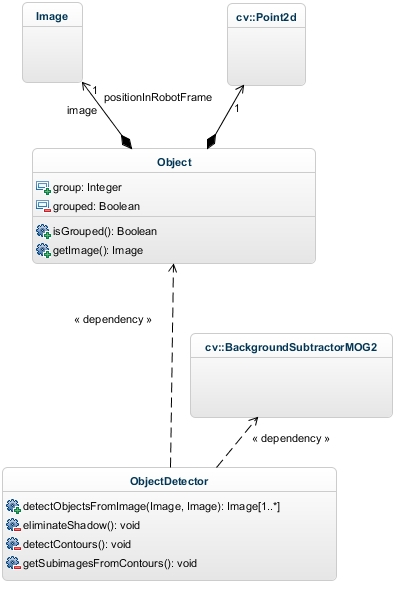
\includegraphics[scale=0.9]{22.eps} 
            \caption{Object Detector classes}
            \label{detector}
        \end{figure}
    % \newpage
        In figure \ref{cluster}, the clustering classes were designed in such a way that other algorithms might be easily added. The abstract class implements the basic functionality and distinguishes the subclasses by names -- an algorithm is identified by its name. 
        \begin{figure}[t!]
            \centering
            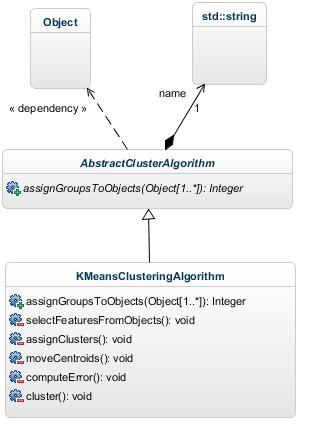
\includegraphics[scale=0.85]{23.eps} 
            \caption{Clustering classes}
            \label{cluster}
        \end{figure}
        In figure \ref{speech} the dependencies of the \verb|Speech| class are shown. This class wraps Text-To-Speech, Speech Recognition and Audio Source Localization functionality. It offers the possibility to speak, hear and determine the approximate position of the speaker.
        \begin{figure}[b!]
            \centering
            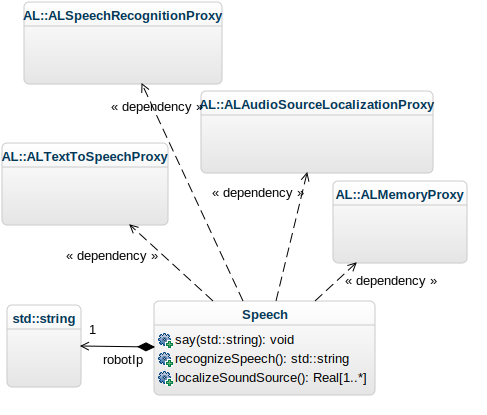
\includegraphics[scale=0.85]{24.eps} 
            \caption{Speech classes}
            \label{speech}
        \end{figure}
% \newpage

        \begin{figure}[b!]
            \centering
            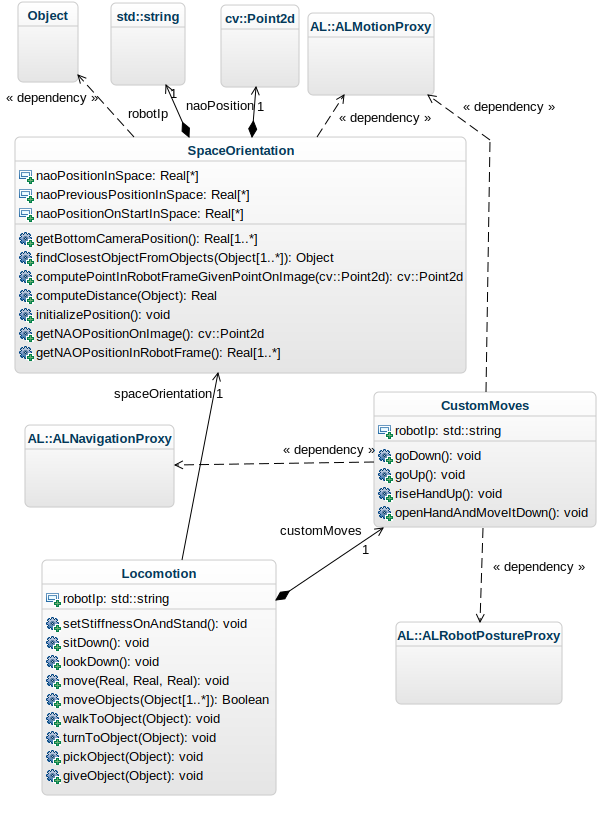
\includegraphics[scale=0.9]{25.eps} 
            \caption{Locomotion and Space Orientation classes}
            \label{locomotion}
        \end{figure}

               In figure \ref{locomotion} it is shown how NAO should perform its movements. But before moving, he needs to know where to move. The class \verb|SpaceOrientation| has this responsibility. The class \verb|SpaceOrientation| is going to be later integrated into \verb|Head| class, while \verb|Locomotion| is more about body itself, so it is a component of \verb|NAO| class, as \verb|Head| itself. But \verb|Locomotion| needs to know about \verb|SpaceOrientation|, so that's why there is an association. The \verb|SpaceOrientation| class computes the distances, performs transformations from one coordinate system to other and retrieves robot's position from sensors. The class \verb|CustomMoves| implements the movements which required Animation Mode to be recorded. Since they are quite specific, they were separated into a different class. Class \verb|Locomotion| has the functionalities like changing robot posture, looking down, perform a generic movement, walk to an object, turn to it, pick it or give it and the method \verb|moveObjects|.
           \begin{figure}[b!]
            \centering
            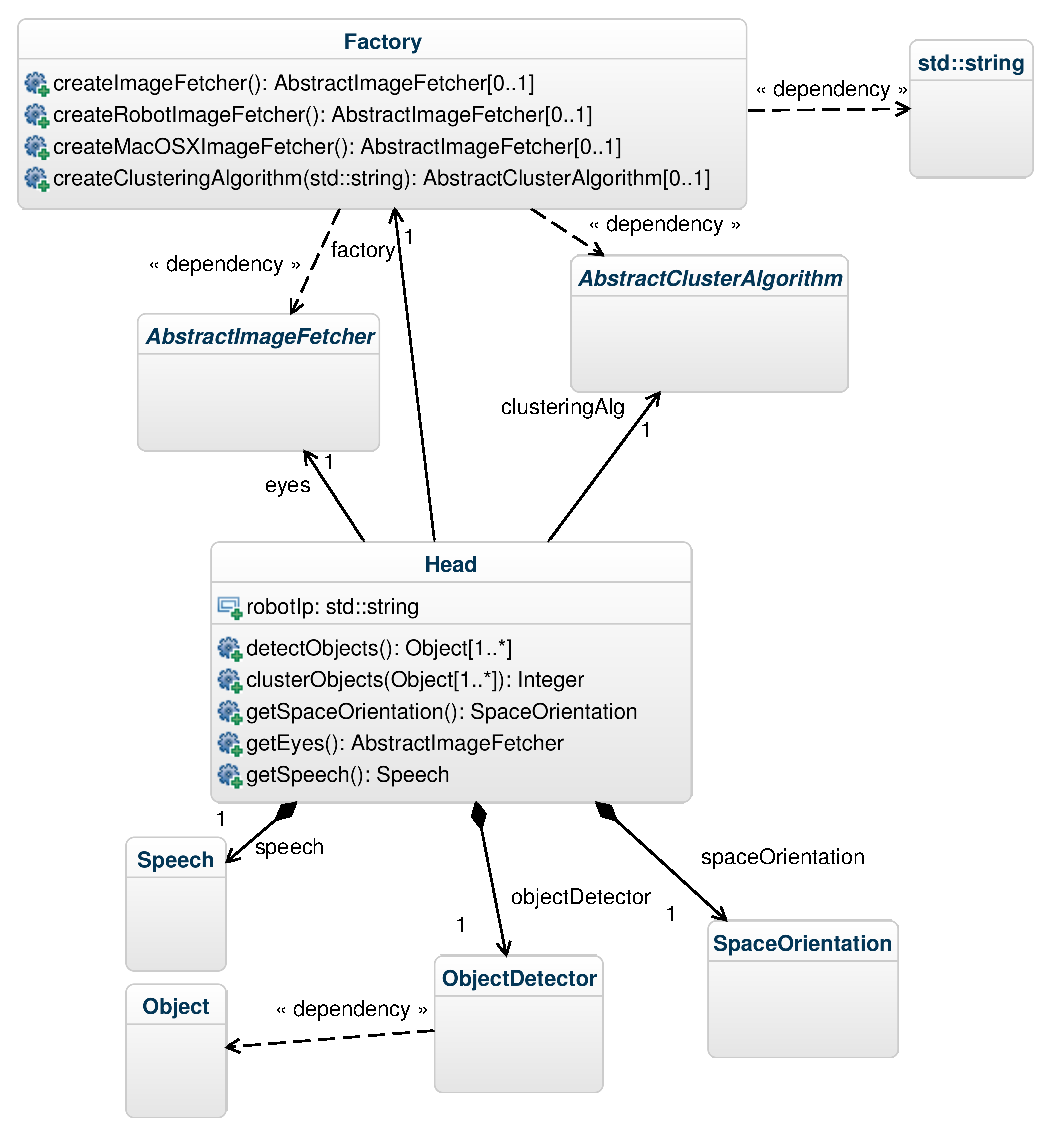
\includegraphics[scale=0.9]{26.eps} 
            \caption{Head class}
            \label{head}
        \end{figure}
        Figure \ref{head} depicts how the class \verb|Head| encapsulates the functionality of speech, object detection and recognition, object clustering and space orientation. At the same time, the \verb|Head| class is decoupled from other specific classes, like \verb|Camera| or a concrete \verb|KMeansClusteringAlgorithm| -- later a different algorithm might be used, or the possibility to choose at runtime the algorithm might be included. That is why the \verb|Factory| design pattern was used. The \verb|Head| class also acts like a facade for the rest, stressing the most important methods of the others. It offers two important methods: \verb|detectObjects| and \verb|clusterObjects|. It also offers access to its members, like \verb|getSpeech| or \verb|getSpaceOrientation|.

        Finally, \ref{naoClass} plays also a role of a facade, but a more general one. It incorporates both \verb|Head| and \verb|Locomotion| and offers functionality like \verb|startInteraction| and \verb|executeCommand|, which are generic for any human-robotic interaction. It also offers public access to its members through getters. 
                To understand how to use these classes and how instances of them interact, the sequence diagram of the whole cycle is presented in figure \ref{sequence} in  Appendix B.
        \begin{figure}[h!]
            \centering
            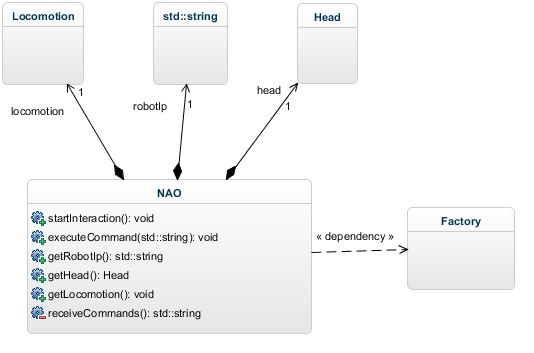
\includegraphics[scale=0.8]{27.jpg} 
            \caption{NAO class}
            \label{naoClass}
        \end{figure}
 

        % \begin{figure}[h!]
        %     \centering
        %     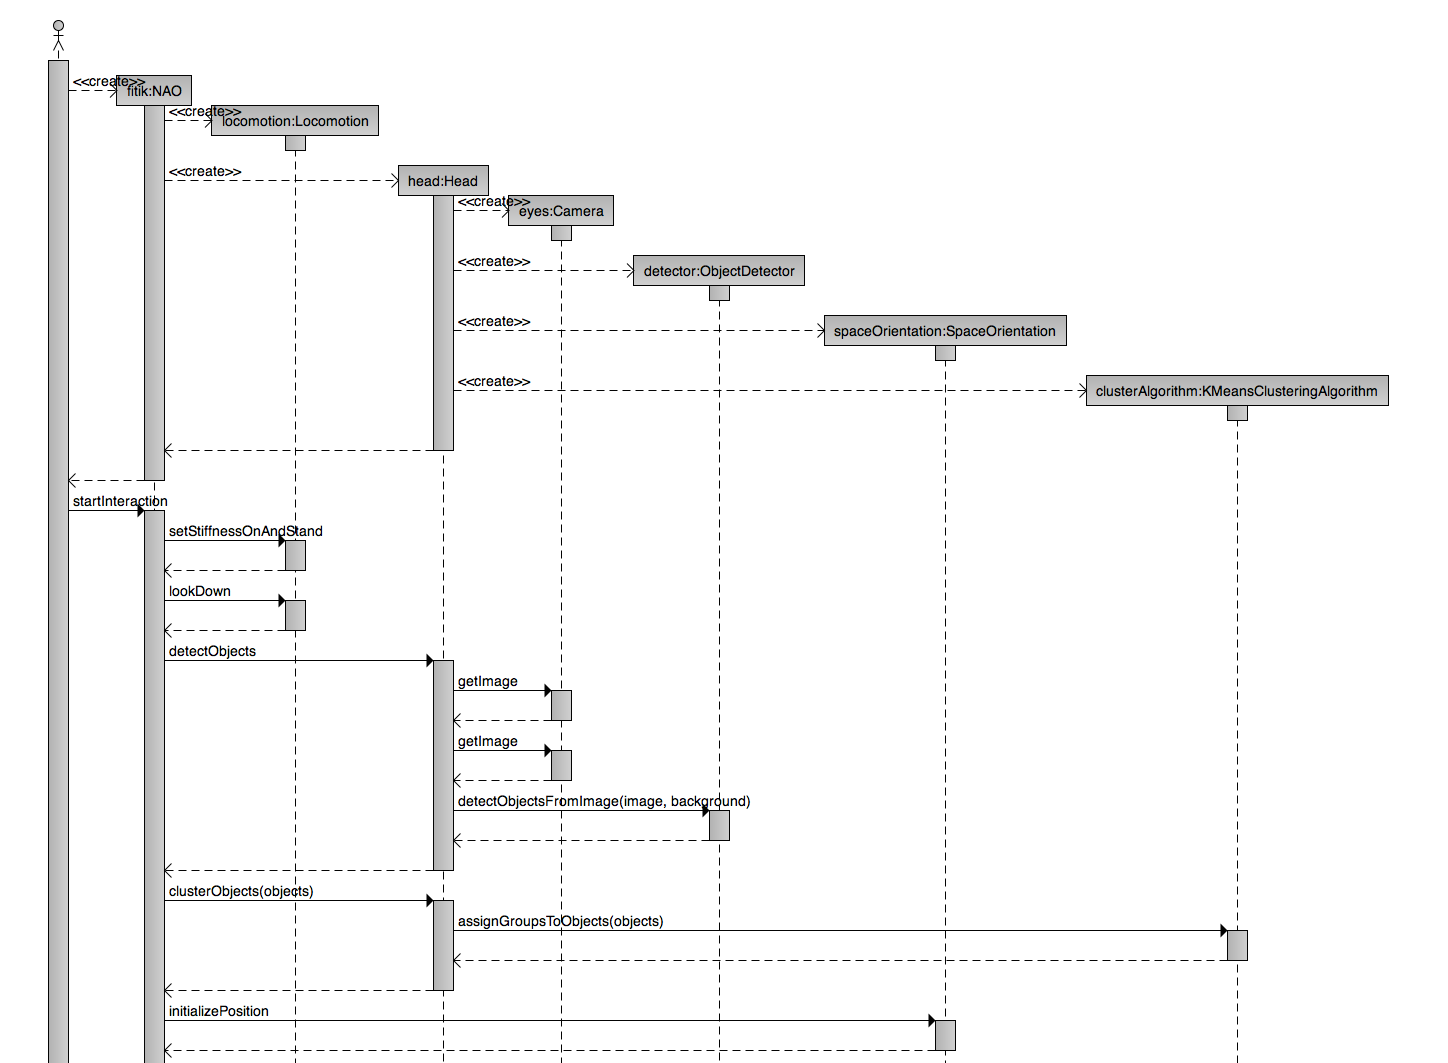
\includegraphics[scale=0.45, angle=90]{28.png} 
        %     \caption{Object interaction -- part I}
        %     \label{sequence1}
        % \end{figure}


        % \begin{figure}[h!]
        %     \centering
        %     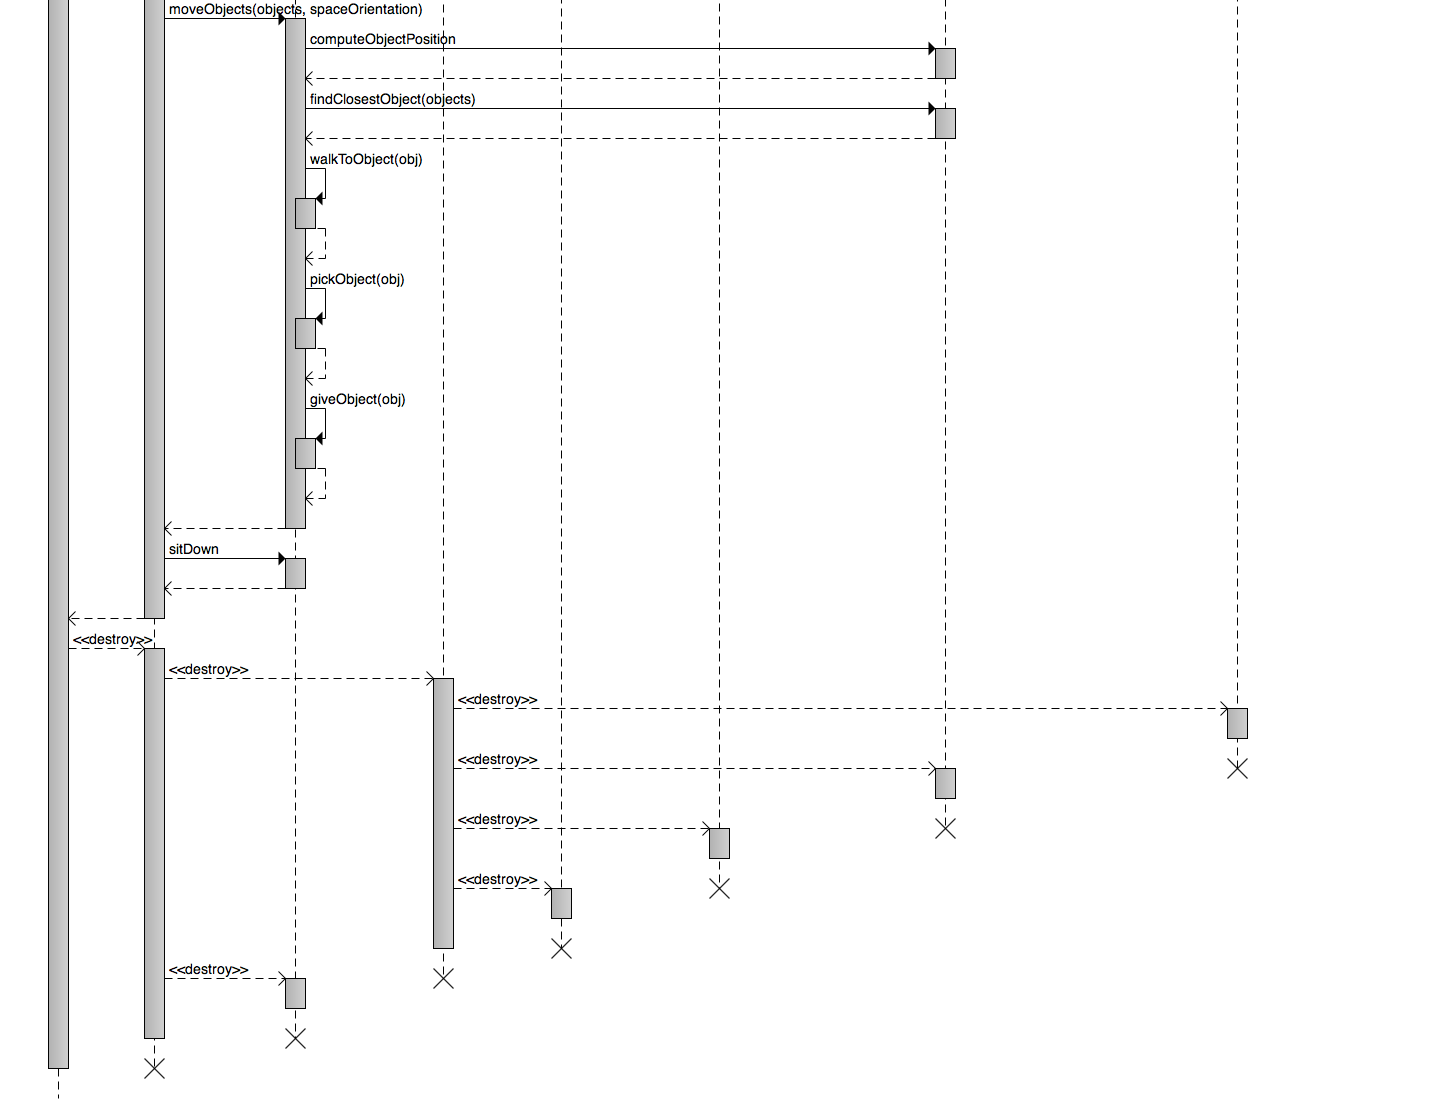
\includegraphics[scale=0.45, angle=90]{29.png} 
        %     \caption{Object interaction -- part II}
        %     \label{sequence2}
        % \end{figure}






\subsection{Implementation}
    \subsubsection{Learning stage}
        Before starting this project, the needed specific technologies and practices should be learned. This project is basically concerned with three topics: NAO robot, OpenCV and Machine Learning. Machine Learning was learned through available free online courses. The first one is available on iTunesU platform, called ``Learning from Data'', tought by professor Yaser Abu-Mostafa, Caltech University. The second one is available from Coursera platform, called ``Machine Learning'', tought by head of Stanford AI lab, Andrew Ng, Stanford University. Both courses include video lectures, slides and homeworks available to download. The only tool required at this stage was Octave, a high-level interpreted language, primarily intended for numerical computations, which is the free version of MatLAB. OpenCV has a great documentation on its official site, with examples and source code. This library is cross-platform, so its installation is the only prerequisite to use it. It was both installed of Linux and Mac OS X.

         NAO was studied using the software which comes with it -- Choreographe. Choreographe has a 90 days free trial period, but also 25 licences are given with the robot. The NAO documentation, available online has a detailed description how to get started or perform some more advanced things with the robot. There is also a community of NAO developers, where different applications are available. So in order to test robot, Choreographe and Webots were installed. Because the C++ SDK is not available for free, Java SDK was used for testing. Later, the installation of C++ SDK have not succeeded on Mac OS X platform. Since Linux was needed anyway and the work was done on two platforms, VirtualBox was installed and a version of Ubuntu on it. On Linux, Qt Creator IDE was installed and additional packages on which the NAO SDK was dependent. After that the C++ SDK was installed and successfully tested. Besides online resources, knowledge was also acquired through discussions with students and consultations with professor Miroslav Skrbek. 

    \subsubsection{Planning}
        The planning of the work was done through asking and answering the right questions. The first two important questions are:
        \begin{enumerate}[topsep=2pt, partopsep=0pt,itemsep=0pt,parsep=1pt]
            \item What the robot can already do;
            \item What the robot cannot do.
        \end{enumerate}
        Studying its capabilities the conclusion was reached, that some actions are very easy to implement, while others are not so intuitive as they may seem (any generic action, not related to this problem). Abstraction is a powerful technique which can be applied for solving any generic engineering problem. Excluding what is irrelevant and leaving only the key points of the problem simplifies it and directs which actions should be done first. Without taking small details into account, there are three subproblems of the main task:
        \begin{enumerate}[topsep=2pt, partopsep=0pt,itemsep=0pt,parsep=1pt]
            \item Detecting an object from the whole picture;
            \item Clustering it;
            \item Moving it.
        \end{enumerate}
        Any subproblem can be divided again in sub-subproblems, recursively, until the current tasks are simple enough to be solved. Then, the solution is built in reverse order, by sticking together the bits. Applying the same Divide \& Conquer method, the following ideas were forumalted:
        \begin{enumerate}[topsep=2pt, partopsep=0pt,itemsep=0pt,parsep=1pt]
            \item teach the system to detect that there are objects; start with one object;
            % \item perform the learning on a computer; the first two steps can be done on a PC, without the need of robot;
            \item teach robot to pick up things;
            \item for increasing the probability of correct matching let him analyze the picked object;
            \item the task is to move the object -- if picking is difficult, object might be dragged.
        \end{enumerate}
        Taking these things into account, the following stages of development were introduced:
        \begin{enumerate}[topsep=2pt, partopsep=0pt,itemsep=0pt,parsep=1pt]
            \item study of Machine Learning -- 1 month;
            \item study of the robot -- 1 month;
            \item study of OpenCV -- 2 weeks;
            \item system design -- 1 week;
            \item system implementation -- 2 months;
            \item testing and analysis -- 2 weeks.
        \end{enumerate}

    \subsubsection{System development}

        The work was started on Mac OS X platform. At the start, Test-Driven Development was used to assure the quality of the code. Latter it was abandoned in favor of time gain. As mentioned, the first two steps did not require the robot so object detection and clustering could be performed on a PC. At first, some draft-programs were written to test the usage of OpenCV. Following some tutorials, it was clear that using \verb|findContours| OpenCV function it is possible to detect the objects. But to detect meant to get their coordinates in the image and the bounding rect so that the sub images might be extracted. Moreover, there were a lot of contours found. Some of them repeated the same shape of one object, some designated just some small dots or shadows -- these were errors. But the \verb|threshold| function gave the possibility to cut dramatically the number of detected contours. As later suggested, many of them were very small, so the filter them one could use the area of that closed contour. The contour could be easily approximated to some polynomial and a polynomial might give the rectangle in which it is enclosed. But detecting objects just from one image was challenging -- that would impose a necessary condition to have a background of one color, without noise. Even with that condition satisfied, the algorithm mistakenly detected shadows as objects. It was a version of detection, which had many disadvantages but it worked.

        After that, a project was created and the basic classes which are indicated in the diagrams were defined, but without a proper implementation yet. It was to assure that the whole skeleton of the application is feasible. A little bit later, this project was added to a git repository, to assure versioning control. A beta-version of object detection was implemented, so the implementation could proceed to the clustering step. Since a custom clustering algorithm was already implemented in MatLAB during online course homeworks, it was ported in C++. Due to the complexity of the real-life machine learning application, the test algorithms are always run on simple points. After different parameters are adjusted, they might be transformed for real examples. Since clustering is Unsupervised Learning, it did not require training. That also meant that it did not require a training data set. At first, the clustering was implemented without Elbow method. The complexity of the implementation of each module was iteratively increased, with each iteration. 


        It was needed to extract somehow features from images. To start simple, only a few were chosen at first iteration. There are as many features as many information bytes in the image. Any pixel of an image can basically be a feature. But due to expensive in processing power algorithms involved in clustering and also due to the fact that clustering itself was repeated many times until the best solution was found, it was unaffordable to use the entire matrix of pixels as features. The simplest way to compare the objects is by comparing their size. So just two features were initially used: the width and the height of the image. An artificial, test image was created with simple shapes as presented in the figure \ref{simpleShape}. The four rectangles, all of the same color but of two different sizes were a good candidate for the start. As the output, OpenCV presented the same image with the detected objects circled with different colors. Each color was associated with a cluster. In a different test, some of the rectangles were rotated by 90 degrees. It caused problems, since the width was associated with the height. Thus all the detected images need first to be preprocessed -- they should be turned in such a way that width is always smaller than the height. 

        % Later, the complexity of the features was increased, taking into account the main colors as well. 

        The implementation of Elbow method was added. It computed the error at every cluster number and looked how dramatically did the error decrease compared to the previous error. The clustering module was tested again with a test image, but this time with different shapes, different colors and multiple clusters. The module successfully determined how many clusters are there and which object goes to which group. Tests also detected numerous wrong groupings, thing which was taken latter into consideration, adjusting the features and other parameters. After the clustering stage was good enough, the module was tested with a real photo. It performed much worse then on simulated images, mostly because of the shadows and light conditions. The problem lay in object detection not in clustering. The background was not so ordinary, it varied from place to place. In a try to tackle that, a method which would recolor the main color was written. It allowed some variance and all the pixels which fell into that range were recolored. That solved the problem but only partially, since now some objects which were slightly of a different color were considered background as well.

        \begin{figure}[t!]
            \centering
            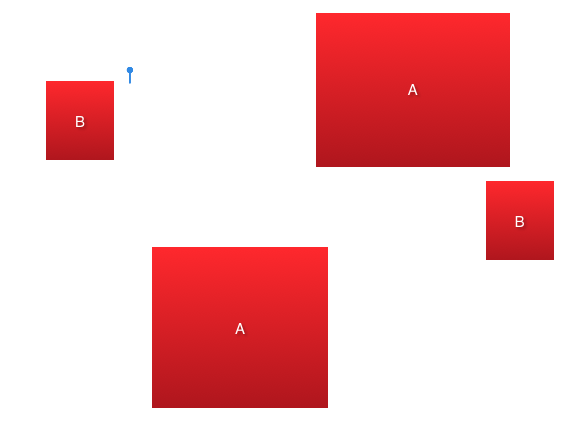
\includegraphics[scale=0.4]{30.png} 
            \caption{Test image for detection and clustering}
            \label{simpleShape}
        \end{figure}

        In the mean time, the project was ported to run on Linux as well, with only difference being the usage of the SDK. The cross-compiled code was written using preprocessing directives, like \verb|#ifdef|. While the program runs on OS X, it retrieves the image from the filesystem and the end result is just a picture with circled objects, sorted in the image. On Linux, program called the needed NAO modules to perform the real moves. So the same modules were tested on NAO, but now the robot retrieved the image from the real camera, and spoke back the results. To test such behavior, the simulator was used. The simulator has limited capabilities, since no speech or its recognition is possible. Another problem was that NAO did not have any grasping functionality implemented. There were no predefined moves for hands and the whole body to reach an object as well. The solution was to use the Animation Mode to define these moves. The robot records the movements of the parts of his body and later they can be reproduced. These movements were then adjusted in Choreographe. The main difficulty in this task is to create such a transition from stand posture to grasping posture that the robot would not fall down during it. Such a movement was obtained only in the last stage of development. 

        After running the project on robot it became obvious that even 50cm for robot are like 2m for a human -- he needs first to walk to an object, then perform that custom movement of grasping. But it was first necessary to know the location of the object in space, in order to know where to move. The analysis of possible ways to compute the distance was done. The most straightforward way is to compute the distance as explained in one of the previous chapters. The height and \( x \) offset of camera were computed from the available sources and robot schemes. Also the corresponding angles were computed. Later a method from SDK which returns these values was used. Since the precision of distance calculation was important, so was the precision of NAO movement. Unfortunately, the precision is quite bad. The robot is biased to the left while moving forward, also performing a small rotation. A small mistake is done during lateral movement as well. Although a compensation of these errors was done, the measurements of errors were not so precise themselves. The errors were a little bit chaotic and it was quite difficult to catch them. This is perhaps the biggest problem still unsolved. 

        After a short research about other functionalities available in OpenCV, it was decided to update the way the objects were detected. It is complicated indeed to make sense what is the background and where are the objects just from one image, especially if the background has some objects drawn on it. The different approach was to use two images -- one of plain background and the next one already with objects. The subtraction is performed and this gives a great mask which can be used later. This method proved to be very good, both independent of background coloring and shadows. After updating the detection method, the system altogether started working better. 

        % The size of the objects which NAO handles and is able to grasp is very small. Not only the size is the problem, but also because of three fingers, some hard solid objects just slide out of his hands while grasping. Only soft objects could be grasped by robot. His fingers are also quite weak and when he tries to close his hand and he meets resistance to this action, he abandons the move. 

        The difference between simulated robot and the real one added some complexity to the task. Some things went quite smoothly in the simulator, but failed on robot. The main problem was the locomotion. Because in the simulator the process was always started from zero the robot was loaded again and all the absolute values which he stores were reset. That is why it was unclear at first that the position which robot retrieves was absolute, but not relative. At every simulation, this absolute position was reset. Because it was reset, all the values indicated zeros and did not influence the distances which robot needed to move. On the other hand, on real robot, these values were not reset and added different biases (being different from zero) and caused the robot to move in almost unpredictable manner. Since this position was not retrieved from the robot's sensors, but by summing up all the previous moves, this data became quite random. It was random because the robot was moved, rotated and transported from place to place by humans -- changes which were not taken into consideration by that data. Finally, the solution was to store the position every time the application run and take it as the origin of coordinates in \verb|FRAME_ROBOT|.

        The robot could detect objects, sort them in some simple way and the basics of locomotion was implemented. At this stage a massive refactoring was done, each class gained a more specific responsibility. The need of some design patterns was revealed. Some abstractions were introduced and common functionality was separated into base classes. To perform the grasping movement, the corresponding movement from Choreographe was exported. The robot was manipulated while the specific positions were recorded. These positions are placed on a timeline and an interpolation between them is done. In such a way, a movement is created. This movement is later exported form Choreographe as a block of code.  

        A set of tests was run to compare the clustering algorithms -- the one available from OpenCV with the one implemented by myself. The tests showed that the library algorithm is better. So the clustering class was updated to use the specific OpenCV functionality. Speech functionality was updated: NAO now said when anything was going wrong. The basics of speech recognition was implemented. Next, the interaction itself with the robot was defined -- everything happens in a infinite loop, in which the robot receives commands and interprets them. The interaction stops when the corresponding command is met. The module with the distance computation was many times updated and changed. Later it was clear that there is no need for the robot to turn (to rotate) -- the way he moves makes him able to reach an object just using the walking feature. 

        The rising of hand was implemented in a similar manner as grasping -- using Animation Mode. It is possible to create such custom movements even without the real robot, but just using the virtual model available in Choreographe. Finally robot successfully traversed the objects. The traversal itself is performed in the following way: NAO selects the closest object to himself and goes to it. It goes down, grasps it and goes up. It gives the object and says to which group it belongs. After that, the process repeats. So in such a way it traverses the objects. But at this stage, NAO does not pick the object, but just goes from one object to other. In the end the grasping functionality was implemented.  This real robot, unlike the one simulated has a error of movement precision. The last stage of development was concerned with compensating these errors, the problem which still remains unsolved. 


    \subsubsection{Results}

        The results show that the project did not achieve its practical goals. The robot was not able to sort the objects due to high mistakes in movement precisions. Nevertheless, during the implementation some interesting achievements were reached. The method of calculation of the distance is both precise and easily reusable in a wide range of tasks. It might be the primitive way to make a robot achieve a 3-D vision. The object detection works flawlessly. It is able to detect objects on almost any background and is able to take shadow into consideration. The illumination though can still affect the result. The clustering is also good, but other algorithms might be used later as well. More features need to be added to make the sorting more elaborate. The system can decide itself the number of clusters. 

        The future work implies refining the current functionality, making the execution local instead of remote and solving the problem of precision. The grasping is difficult due to the number of fingers. The project runs both on Linux and Mac OS X. The Mac OS X functionality needs to be extended, so that remote execution on robot worked from there as well. Similar program should run on Windows platform as well. This project can serve as a detailed analysis of humanoid's capabilities mostly concerned to interaction with objects and humans. This project also presents a successful example of interaction between three components from different branches of IT: robotic functionality, image processing and machine learning. This work itself might be interesting and useful in future robotics research and improvements, both concerned with NAO and other robots as well. 






\clearpage
\cleardoublepage
\addtocontents{toc}{\protect\thispagestyle{empty}} % no page number on the table of contents page

						%CAPITOLUL 4
						% \input{Chapter_4.tex}
						% \cleardoublepage

%CAPITOLUL 5
\section{Economic Analysis}
\phantomsection

	\subsection{Project description}

	Robotics and AI are at the edge of today's technology and most probably will play an important role in humans' lives in the close future. This is the reason why such projects have a high degree of importance from economical point of view. While today there not so many commercial products in these areas compared to other areas from IT, there are still bold investments and funding in research and commercial companies. Every day more and more new commercial products concerned with robots and AI appear. 
  	The current project is concerned with creating a detailed analysis and research about interaction between the robot and the physical world around him. The robot has to sort some objects -- a task met by humans many times in everyday life. It has to identify them and group them. Even if this is not a fully-backed commercial app which can be placed on store, it still has economical insights. Moreover, NAO robot community is young but quickly-growing one, and has a software store as well. So even the research projects in this area can be made business projects. The project is concerned with different ``hot'' technologies, like Computer Vision or Machine Learning. OpenCV, with its image processing algorithms is actively supported by people all around the world, including big companies. Machine Learning specialists are hunt by major companies in the industry. Because of all of the above, this system requires an economical analysis as well.

	\subsection{SWOT analysis}

	SWOT analysis is the analysis of project’s strengths and weaknesses, opportunities and threats from different points of view, including economical one. It is important to predict how well a product would succeed on the market, in order to comply with revenue expectations and prepare for possible risks. A research can be judged in such a way as well. The analysis of this project is presented in table \ref{swot}.
\begin{table}[ht!]
\centering
\caption{SWOT Analysis}
{
\renewcommand{\arraystretch}{2}
\begin{tabular}{ l|l }
\hline           
 \pbox{4cm}{\textbf{Strong points}} &\pbox{5cm}{\textbf{Weak points}} \\ \hline \hline
 {-- sorts any objects;} & {-- works only in laboratory conditions;} \\ 
 {-- works on any background;} & {-- there are mistakes in movement precision;} \\ 
 {-- decides by himself how to group the objects;} & {-- the robot itself is still unpractical;} \\ 
 {-- the robot interacts by voice;} & {-- has a low percentage of grasping.} \\ 
  {-- the robot identifies the speaker position;} & { } \\ 
  {-- correctly identifies the objects;} & { } \\ 
  {-- correctly determines the object’s position.} & { } \\ \hline

 {\textbf{Opportunities}} & {\textbf{Threats}} \\ \hline \hline
 {-- can be easily extended or integrated;} & \pbox{8cm}{-- in rear cases, robot can fall down during his movements;} \\ 
 \pbox{8cm}{-- the future versions can be used in practical tasks like cleaning the room;} & \pbox{8cm}{-- robot can group the objects in a way other than desired by humans;} \\ 
 {-- modules are independent and reusable;} & \pbox{8cm}{-- the algorithms of movement can be upgraded to use real-time image processing.} \\ 
 \pbox{8cm}{-- the clustering module in its generic form can be upgraded to make NAO learn independently the world around him.} & { } \\ \hline
\end{tabular}
}
\label{swot}
\end{table}

By taking a look at SWOT analysis it can be concluded that the project has both strong and weak points, and the ability to tackle them and use of correct marketing techniques will help to present and sell the solution in a better way. Opportunities and threats present a superficial prediction of where this project is evolving, what possibilities for growth and downfalls it has.
		

	\subsection{Project time schedule}

	Time is perhaps one of the main resources in any work. The expenses of manufacturing a product are directly proportional with the amount of time needed for that. This implies the importance of having a schedule. Because of lack of experience in general and especially in the field of robotics, it is difficult to predict how much time will this project need. There is also a probability that the result of the work would not satisfy the requirements (that is, how feasible the actions done by robot are). All these need to be taken into account to approximate the timeline of work. When computing how much time a project would require, it is useful to also leave some buffer zone -- reserve time -- just in case it is not fitting the schedule. The timeline depends on the activities there would be done. These activities are determined by objectives the project has. 
  % These activities are determined by objectives the project has. These activities are determined by objectives the project has. 

		\subsubsection{Objectives}

		The main objective of this project is to make NAO robot sort a set of objects. This implies the steps that the robot needs first to identify the objects, then cluster them and finally move them. A secondary objective is to make NAO autonomous and independent, so that without human’s assistance he would be able to move around objects in the room as he wishes. From economical point of view, the main objective of this research is not to sell the solution, but to attract interested companies and get a positive feedback from the community, making this work useful and interesting.

		\subsubsection{Schedule}

		An IT project consists of five important phases:
        \begin{enumerate}[topsep=0pt, partopsep=0pt,itemsep=0pt,parsep=1pt, itemindent=1cm]
        \item Planning;
        \item Research;
        \item Implementation;
        \item Validation;
        \item Launch.
        \end{enumerate}
        Each one of such phases consists of many smaller steps, sub-blocks. In this project, the work was done in an iterative model, each time incrementing the complexity of the implemented solution.
    	The people involved in the development are:
    	\begin{enumerate}[topsep=0pt, partopsep=0pt,itemsep=0pt,parsep=1pt]
        \item Project Manager (PM) — he will coordinate the work between the developer, product owner and the researcher;
        \item Software Developer (SD) — he will design and develop the application, as specified by the requirements;
        \item Researcher (R) — he will design the algorithms and approaches in human-robotic interaction, image processing and AI;
        \item Product Owner (PO) — he is the main stakeholder, interested in the result of the project and research.
        \end{enumerate}
        The total duration of the project is represented by the formula \ref{duration}.
      \begin{equation}
      \label{duration}
      	D = D_{S} - D_{E} + R,
        \end{equation}
        where \( D\) is the duration, \( D_{S}\) is the start date and \(D_{E}\) is the end date. \(R\) represents the reserve time.
        Using the above information and formula, the initial schedule of the project is presented in table \ref{schedule}.
        \begin{table}[hb!]
\centering
\caption{Project schedule}
{
\renewcommand{\arraystretch}{2}
\begin{tabular}{ c|c|r|c|c }
\hline           
 {\textbf{Nr.}} & \pbox{6cm}{\textbf{Activity name}} &\pbox{2cm}{\textbf{Duration \newline(days)}} &\pbox{2cm}{\textbf{Workers}} &\pbox{5cm}{\textbf{Resources Used}} \\ \hline \hline
{1} & \pbox{6cm}{Analysis of tasks} & 2  & \pbox{2cm}{PM, SD, PO, R} & \pbox{5cm}{Internet, PC, office, inventory (paper, pen, etc.)} \\ \hline
{2} & \pbox{6cm}{Requirements definition} & 1  & \pbox{2cm}{PM, PO} & \pbox{5cm}{PC, Internet, office} \\ \hline
{3} & \pbox{6cm}{Study of existent solutions} & 5  & \pbox{2cm}{PM, PO, R, SD} & \pbox{5cm}{Internet, PC, office, books} \\ \hline
{4} & \pbox{6cm}{Study of robot}  & 10  & {SD} & \pbox{5cm}{robot, PC, office, Internet, book, robot simulator} \\ \hline
{5} & \pbox{6cm}{Functional design of the system (use-case diagrams)} & 1  & {PM, PO} & \pbox{5cm}{PC, office, UML tool, Internet} \\ \hline
{6} & \pbox{6cm}{Interaction design of the system (sequence diagrams)} & 1  & {PM, SD} & \pbox{5cm}{PC, office, UML tool, Internet} \\ \hline
{7} & \pbox{6cm}{System structural design (class diagrams)} & 2  & {PM, SD} & \pbox{5cm}{PC, office, UML tool, Internet} \\ \hline
{8} & \pbox{6cm}{Workflow design (state and activity diagrams)} & 2  & {PM, SD} & \pbox{5cm}{PC, office, UML tool, Internet} \\ \hline
{9} & \pbox{6cm}{Interface design} & 4  & {PM, SD} & \pbox{5cm}{PC, Internet, office} \\ \hline
{10} & \pbox{6cm}{Choice of algorithms and techniques} & 5  & {R, SD, PM} & \pbox{5cm}{PC, Internet, office, books} \\ \hline
{11} & \pbox{6cm}{System Implementation} & 20  & {SD} & \pbox{5cm}{PC, office, robot, robot simulator, Internet} \\ \hline
{12} & \pbox{6cm}{Testing and adjustments} & 30  & {SD} & \pbox{5cm}{Robot, simulator, PC, office, test objects} \\ \hline
{13} & \pbox{6cm}{Project documentation} & 10  & {PM, SD} & \pbox{5cm}{PC, Internet, office} \\ \hline
{14} & \pbox{6cm}{Project presentation preparations} & 4  & {PM} & \pbox{5cm}{PC, Internet, office} \\ \hline
\multicolumn{1}{c}{} & \multicolumn{1}{c|}{\pbox{6cm}{Total days to finish the system}} & {96} \\ \cline{1-3} %\multicolumn{2}{|c}
\end{tabular}
}
\label{schedule}
\end{table}
The table \ref{schedule} depicts the actions necessary to realize the project, the time required for each action, and the workers and resources needed for that. The total time needed to complete the project is estimated to 96 days.
\begin{itemize}[topsep=5pt, partopsep=0pt,itemsep=3pt,parsep=1pt]
\item[--] PO (product owner): 9 days;
\item[--] R (researcher): 12 days;
\item[--] PM (project manager): 36 days;
\item[--] D (developer): 90 days.
\end{itemize}


	\subsection{Economical proof}

	To evaluate this project from economical point of view, the expenses of it should be computed. These expenses are divided in the following groups: tangible, intangible, salary and indirect expenses. This is a non-commercial project so there are no profit estimations, nor financial results. In this section all the expenses, including the salary for a developer, wear and depreciation of materials will be computed. The computing of the budget will include the money necessary to buy all tangible and intangible assets, indirect expenses as well as salaries.


		\subsubsection{Tangible and intangible expenses}

		To compute the budget that is needed for the project, it is required to estimate the tangible and intangible assets. The list of the material assets are presented in Table \ref{tangible}.
\begin{table}[ht!]
\centering
\caption{Tangible asset expenses}
{
\renewcommand{\arraystretch}{2}
\begin{tabular}{ c|r|r|r }
\hline           
 {\textbf{Name}} & \pbox{4cm}{\textbf{Price (MDL)}} &\pbox{4cm}{\textbf{Quantity}} &\pbox{4cm}{\textbf{Sum (MDL)}} \\ \hline \hline
{NAO H25 NEXT GEN robot} & {110262} & {1} & {110262} \\ \hline 
{PC} & {9000} & {1} & {9000} \\ \hline 
{Photo-camera} & {3000} & {1} & {3000} \\ \hline 
\multicolumn{1}{c}{Total} & \multicolumn{2}{l|}{} & {122262} \\ \hline
\end{tabular}
}
\label{tangible}
\end{table}
Because all the software, applications and programs are either free of charge, offer a trial license or come together with the NAO robot kit, there are no intangible assets.  These are summarized in Table \ref{direct}.
%Besides these expenses, there are also some other direct expenses, logistic products that were used during development.
\begin{table}[hb!]
\centering
\caption{Direct material costs}
{
\renewcommand{\arraystretch}{2}
\begin{tabular}{ c|c|r|r|r }
\hline           
 {\textbf{Nr.}} & {\textbf{Name}} & \pbox{3cm}{\textbf{Unit price \newline (MDL)}} &\pbox{3cm}{\textbf{Quantity}} &\pbox{2cm}{\textbf{Sum (MDL)}} \\ \hline \hline
{1} & {copybook (60 pages)} & {15} & {1} & {15} \\ \hline 
{2} & {rubber ducks} & {30} & {4} & {120} \\ \hline 
{3} & {plastic big balls} & {25} & {4} & {100} \\ \hline 
{4} & {rubber small balls} & {15} & {6} & {90} \\ \hline 
{5} & {printing} & {0.5} & {200} & {100} \\ \hline 
{6} & {pen} & {5} & {3} & {15} \\ \hline 
{7} & {USB flash} & {200} & {1} & {200} \\ \hline 
{8} & {meter} & {20} & {1} & {20} \\ \hline 
\multicolumn{1}{c}{} & \multicolumn{1}{c}{Total} &\multicolumn{2}{c}{} & \multicolumn{1}{|r}{680} \\ \hline
\end{tabular}
}
\label{direct}
\end{table}
This concludes the direct expenses for the project which amounts to 122262 + 680 = 122942MDL.

		\subsubsection{Salary expenses}

		In this section, the expenses necessary to pay the labor personnel will be computed. In order to do that, certain considerations will be taken into account such as the current percentage for the various funds that need to be paid. Besides the wages the social fund and the medical insurance expenses are computed. The salaried are presented in Table \ref{salary}.
\begin{table}[ht!]
\centering
\caption{Salary expenses}
{
\renewcommand{\arraystretch}{2}
\begin{tabular}{ c|c|r|r|r|r }
\hline           
 {\textbf{Nr.}} & \pbox{3cm}{\textbf{Position}} & \pbox{2cm}{\textbf{Number of \newline employees}} &\pbox{3cm}{\textbf{Amount of work(h)}} &\pbox{3cm}{\textbf{Sal/unit (MDL/h)}} &\pbox{3cm}{\textbf{FSB (MDL)}} \\ \hline \hline
{1} & {Product owner} & {1} & {72} & {60} & {4320} \\ \hline 
{2} & {Project Manager} & {1} & {288} & {50} & {14400} \\ \hline 
{3} & {Software developer} & {1} & {720} & {90} & {64800} \\ \hline 
{4} & {Researcher} & {1} & {96} &{120} & {11520} \\ \hline 
\multicolumn{1}{c}{} & \multicolumn{1}{c}{Total} & \multicolumn{3}{c}{} & \multicolumn{1}{|r}{95040} \\ \hline
\end{tabular}
}
\label{salary}
\end{table}
Having the salary information, it is necessary to compute how much to pay to the social service fund, the medical insurance fund, and the total work expenses that will be obtained by summing those up. \( F_{re} \) stands for ``Fondul de Retribuire a Muncii'' and is equal to:
      \begin{equation}
      \label{duration}
      	F_{re} = 4320 + 14400 + 64800 + 11520 = 95040
        \end{equation}
The social service expenses will be equal to:
      \begin{equation}
      \label{duration}
      	FS = F_{re} \cdot T_{fs} = 95040 \cdot 0.23 = 21859,
        \end{equation}
where \( T_{fs} \) is the contribution quota for the state mandatory social insurance, approved each year by Law of Budget (in 2014 — 23\%). Now the medical insurance fund is computed as
      \begin{equation}
      \label{duration}
      	MI = F_{re} \cdot T_{mi} = 95040 \cdot 0.04 = 3801,
        \end{equation}
where \( MI \) is medical insurance and \( T_{mi} \) is the medical insurance quota approved each year by the Law of Budget for state medical insurance (in 2014 — 4\%).
\newline The total work expense fund can be computed as follows:
      \begin{equation}
      \label{duration}
      \begin{split}
      	WEF = F_{re} &+ FS + MI = \\ 95040 + 21859 &+ 3801 = 120700,
        \end{split}
        \end{equation}
where \( WEF \) is the work expense fund.

		\subsubsection{Indirect expenses}

		The indirect expenses of the project are computed -- this includes the expenses that cannot be added to the direct ones and are things like electricity, internet, water, etc. The indirect expenses are shown in Table \ref{indirect}.
\begin{table}[hb!]
\centering
\caption{Indirect expenses}
{
\renewcommand{\arraystretch}{2}
\begin{tabular}{ c|c|c|r|r|r }
\hline           
 {\textbf{Nr.}} & \pbox{3cm}{\textbf{Name}} & \pbox{4cm}{\textbf{Unit of measurement}} &\pbox{3cm}{\textbf{Quantity}} &\pbox{3cm}{\textbf{Tarif (MDL/unit)}} &\pbox{3cm}{\textbf{SUM (MDL)}} \\ \hline \hline
{1} & {Power usage} & {kWh} & {480} & {1.58} & {758} \\ \hline 
{2} & {Internet} & {month} & {4} & {120.00} & {480} \\ \hline 
{3} & {Office rent} & {month} & {4} & {200.00} & {800} \\ \hline 
{4} & {Cleaning} & {month} & {4} &{300.00} & {1200} \\ \hline 
{5} & {Meals} & {month} & {4} &{600.00} & {2400} \\ \hline 
\multicolumn{1}{c}{} & \multicolumn{1}{c}{Total} & \multicolumn{3}{c}{} & \multicolumn{1}{|r}{5638} \\ \hline
\end{tabular}
}
\label{indirect}
\end{table}

		\subsubsection{Wear and project cost}

		An important part of indirect expenses is the computation of wear and depreciation of assets. The depreciation should be computed uniformly for the project duration, so that there are no accountancy issues. That means that if a material is planned to be used for 3 years, it should be divided into 3 uniform parts for each year. The straight line depreciation method will be used. The wear is computed depending on the type of asset. For the notebook and camera, the period of use equals to 5 years. For robot it is 10 years. First the total expenses of the tangible assets are summed up and then the salvage costs of each of the items at the end of their period of use has to be subtracted:
      \begin{equation}
      \label{duration}
      \begin{split}
      	W_{y} = &\frac{C_{i} - C_{s}}{P} = \\ \frac{110262 - 11000}{10 years} + &\frac{9000 - 900}{5 years}  + \frac{3000 - 300}{5 years} =\\ 9926 + &1620 + 540 = 12086,
      \end{split}
    \end{equation}
    where \( W_{y}\) represents the wear per year, \( C_{i}\) is the initial cost, \(C_{s}\) is the salvage cost and \( P\) is the period of use.
        This includes 3 tangible assets — the robot, the PC and a camera. The initial asset value is equal to 122262MDL since no intangible assets are there. It is to be noted that because the project takes 96 days to complete (roughly 4 months), the wear value of the assets should take that period into consideration giving the following amount:
      \begin{equation}
      \label{duration}
      \begin{split}
      	W_{p} = &\frac{W_{y}}{D_{y}} \cdot P =\\ \frac{12086lei}{365days} \cdot 9&6days = 3178,
      \end{split}
    \end{equation}
where \( W_{p}\) is the project wear value, \(D_{y}\) is days in year.
		% \subsection{Project cost}

		Now that the expenses of the project are done, it is possible to compute the product cost which includes direct and indirect expenses, the salary expenses, and the wear expenses. The detailed presentation of expenses is included in the Table \ref{project}. Summarizing, the total project cost is 252458MDL. The robot itself represents 48\% of these expenses.
% \begin{table}[hb!]
% \centering
% \caption{Project cost}
% {
% \renewcommand{\arraystretch}{2}
% \begin{tabular}{ c|r|r }
% \hline           
%  {\textbf{Expense}} & \pbox{3cm}{\textbf{SUM (MDL)}} & \pbox{4cm}{\textbf{Percentage (\%)}} \\ \hline \hline
% {Direct expenses} & {122942} & {48.73} \\ \hline 
% {Salary expenses} & {95040} & {37.64} \\ \hline 
% {Social fund expenses} & {21859} & {8.65} \\ \hline 
% {Indirect expenses} & {5638} & {2.23} \\ \hline 
% {Medical insurance expenses} & {3801} & {1.5} \\ \hline 
% {Asset wear expenses} & {3178} & {1.25} \\ \hline 
% {\textbf{Total product cost}} & \pbox{3cm}{\textbf{252458}} & \pbox{3cm}{\textbf{100}} \\ \hline

% \end{tabular}
% }
% \label{project}
% \end{table}
  		\subsection{Economic conclusion}
  		
  		Because this is a research project and does not result in a commercial product, no profit was computed. But even such a project requires an economic analysis in order to predict its cost and search for investors. A ready business plan can show what to expect and how much someone has to risk or pay to start something. The research was always a good purpose and its gain is not immediate. Instead, through scientific breakthroughs and innovations which happen once in a while the outcome of such projects is tremendous. Looking at the obtained data, it is clear that the main expense is the robot. At the same time, it has twice as long lifetime compared with other assets. Ten years of exploitation is a fair amount of time for technology. Besides that, many more project might be done on him. This project has a considerable cost. Big institutions, like universities or private companies can afford such a project.

\clearpage
\cleardoublepage

% IMPORTANT REMARK  
% If your table of contents need to be splitted in two parts (in order to accomodate the frame used for TOC)
% within the body text, right before the chapter/section that you want to be started on anew page, 
% you should add:     \addtocontents{toc}{\protect\newpage}

%CONCLUZII
\phantomsection
\addcontentsline{toc}{section}{Conclusions}
\section*{Conclusions}
\phantomsection


	NAO is an excellent robot for research, but he still cannot be used for any practical task. His battery drains fast (in one-two hours), and the speed of his movements is low. There are also quite high errors in movement precisions. The initial goal was not reached due to the combination of two factors: static analysis of the current state and errors of precision committed by robot while walking. The analysis is static because NAO computes his position relative to objects using just one image. One solution to this problem might be real-time or close to real-time image processing.

	This project can serve as a detailed analysis of humanoid's capabilities mostly concerned to interaction with objects and humans. K-means clustering with features extracted just from images provides a good way to sort a set of objects. The image of an object contains enough information to represent it. Elbow method is effective in deciding the number of clusters. K-means together with Elbow method solved the core of the problem. Clustering itself in a generic form might be used by robots to learn the world around them, since it is unsupervised learning and the knowledge attained is a result of data which robot takes from its sensors but not from preprogrammed instructions inserted by humans. The implementation of object detection proved to be very effective and independent of background. It is still affected by conditions of illumination. 

	During this project a method of distance determination from image was proposed. The implementation of the program shows that it is possible to compute with high accuracy the distance to an object using just an image and additional knowledge about camera's specifications and its position in space. Knowing the height of the camera and the height angle it is possible to compute the forward distance. The height angle is formed by the line which is the orthogonal projection of the camera center on the ground and the line formed by camera center and the point with camera \( x \) coordinate and object center \( y \) coordinate. Knowing the camera projection distance and the lateral angle it is possible to compute the lateral distance. The camera projection distance is the distance bounded by camera on one end and point of intersection of camera's vector projection with the ground. The camera projection distance can be computed having forward distance. The lateral angle is the angle formed by the camera projection line and object center. Having the forward and lateral distances it is possible to compute both the distance towards the object and the position relative to camera of the object.   

	For object detection a set of OpenCV methods were implemented. Background subtraction and shadow removal were used. The OpenCV method of finding the contours of the objects was implemented. Object detection and object clustering modules can be easily reused in other projects. Distance computation module might be useful for a wide range of tasks performed by NAO. The model of human-robotic interaction implemented here is a generic one and can be easily extended for very different practices. Computer Vision and image processing is still a challenging task. It requires much processing power and complex algorithms to be truly successful and independent of circumstances.

	A vast amount of time was spent experimenting with NAO movement precision and grasping capabilities. It was shown that this specific instance of the robot has one motor of motion biased, resulting in a significant error. The project once again emphasized the issue of grasping with three fingers. While this thesis was being finished, Aldebaran Robotics released the next generation humanoid -- Pepper. Pepper tackles this issue and has five fingers. Experiments were also concerned about NAO's capabilities to detect obstacles and pick an object from the ground without falling down. The program is able to deal with almost any object, any number of groups and any background. This work itself might be interesting and useful in future robotics research and improvements, both concerned about NAO and other robots as well.  

	This project also presents a successful example of interaction between three components from different branches of IT: robotic functionality, image processing and machine learning. Since the main task was not practically achieved, there is much future work to be done. The biggest problem unsolved is the incapacity of the robot to walk exactly the right distance. The problem comes from the biased motors used during walking. But it could be tackled by recomputing the distances and errors from time to time. That way, even if the robot would have imprecise movements, it would compensate his errors until the result is good enough. This requires the processing of the image with objects more than once. It also requires to keep track which object is which in the new, closer image (that is, object recognition besides object detection which is done at the moment). Since the image needs to be processed at least a few times in some short interval, may be even once a second, the program needs to be run locally, on robot. 


	The network image retrieval during remote execution would not permit to respect such short intervals, since to get an image from robot to the PC remotely takes a couple of seconds (for the best resolution image). But running the system on the robot could lead to possible delays during clustering, since the robot's processor is weaker than the one from the PC and the clustering is a computationally expensive operation. This means that an important factor in the future work would be to balance the processing expenses versus the frequency of distance recalculation. Besides that, more detailed features of the objects might be added, increasing the robot's profficiency in sorting even similar objects. Another thing which was not tested is the diversity of the clustering algorithms. Just one of them was implemented. Others might be compared with that as well. Another problem is the grasping itself, which is dependent of the mechanical form of the NAO's hand. Finally, when the robot would be good at sorting things locally, the project can be upgraded to make NAO perform more difficult tasks, like moving the objects around the room. 



\clearpage
\cleardoublepage

\cleardoublepage
\addcontentsline{toc}{section}{References}
\begin{thebibliography}{99999}
\phantomsection
\singlespace\normalsize

% \bibitem{Ak} Akins R.E. Performance evaluation of wind-energy conversion systems using the method of bins - current status. Internal.Report SAND-77-1375. Sandia Laboratory, USA, 1978. 

% \bibitem{And}Anderson J.D., Fundamentals of aerodynamics, 2nd Edition. McGraw-Hill, Singapore.

% \bibitem{booch} Booch G. et. al\textit{., }Object-Oriented Analysis and Design with
% Applications, Addison-Wesley 2007.

% \bibitem{Bostan}
% Bostan I., Dulgheru V., Sobor I., Bostan V., Sochirean A., Sisteme de
% conversie a energiilor regenerabile, Technica-Info 2007.

% \bibitem{Xfoil}Drela M. Xfoil : An Analysis and Design System for Low Reynolds Number Airfoils. Low Reynolds Number Aerodynamics, Springer-Verlag, Lec. Notes in Eng. 54, 1989.

% \bibitem{gamma} Gamma E., Helm R., Johnson R., Vlissides J.\textit{, }Design Patterns -
% Elements of Reusable Object-Oriented Software, Addison-Wesley 1994.

% \bibitem{Larman1} Larman C., Agile and Iterative Development: A Manager's Guide, Adisson
% Wessley 2003.

% \bibitem{Larman2} Larman C., Applying UML and Patterns: An Introduction to Object-Oriented
% Analysis and Design and the Unified Process, Addison Wessley 2002.

% \bibitem{PITAC} President’s Information Technology Advisory Committee, Computational Science: Ensuring America’s Competitiveness, Report to President, \url{http://www.nitrd.gov/pitac/reports/20050609_computational/computational.pdf}, June 2005. 

% \bibitem{CwithUML} \url{http://www.drdobbs.com/184401948}

% \bibitem{Pic1}Super-sized 6.15MW Wind Turbine Up and Running, 2050 Magazine, \url{http://www.2050publications.com/super-sized-6-15mw-wind-turbine-up-and-running/}

% \bibitem{Pic2}Largest Wind Farm in Europe Alive, \url{http://www.renewindians.com/2012/12/Largest-Wind-Farm-in-Europe.html}

% \bibitem{Pic3}GE Power \& Water, Renewable energy, \url{http://www.ge-renewable-energy.com/uploads/tx_spdownloads/Fantanele_Romania_2.xWEA_03.JPG}

	\bibitem{naoDocumentation}
		Aldebaran Robotics.
		\emph{NAO Software 1.14.4 documentation}.
		 \url{www.community.aldebaran-robotics.com/doc/1-14/index.html}

		 	\bibitem{webots}
		Cyberbotics.
		\emph{Webots overview}.
		\url{www.cyberbotics.com/overview}

		 	\bibitem{objectGrasping}
		Egbert van der Wal.
		\emph{Object Grasping with the NAO: master's thesis}.
		Department of AI, 
		University of Groningen,
		The Netherlands.
		\url{www.ai.rug.nl/~mwiering/thesis\_Egbert\_van\_der\_Wal.pdf}

		 \bibitem{naoWiki}
		Endgadget.
		\emph{Nao robot replaces AIBO in RoboCup Standard Platform League}
		\url{www.engadget.com/2007/08/16/nao-robot-replaces-aibo-in-robocup-standard-platform-league/}

			\bibitem{shadowRemoval}
		Fredembach C., Finlayson G.
		\emph{Simple Shadow Removal}.
		\url{www.ivrgwww.epfl.ch/alumni/fredemba/papers/FFICPR06.pdf}




	\bibitem{graspingKnownObjects}
		Gupta A., Frese U., Dawood M.
		\emph{Grasping Known Objects with Aldebaran Nao}.
		\url{www.cse.iitk.ac.in/users/cs365/2012/submissions/ashug/cs365/projects/report.pdf}

 	\bibitem{objectLearning}
		Heinrich S., et. al.
		\emph{Object Learning with Natural Language in a Distributed Intelligent System --
		A Case Study of Human-Robot Interaction}.
		Department of Informatics,
		University of Hamburg.
		\url{www.informatik.uni-hamburg.de/WTM/ps/Heinrich\_CSIP2012\_CR.pdf}

 	\bibitem{visualGrasping}
		Holl T., Pinz A.
		\emph{Vision-based grasping of objects from a table using the humanoid robot Nao}.
		Inst. of Electrical Measurement and Measurement Signal Processing Graz Univ. of Technology, Austria.
		\url{www.emt.tugraz.at/system/files/ARW\_2011.pdf}

		\bibitem{naoPhoto1}
		Image with NAO.
		\emph{Aldebaran Robotics NAO Next Gen Fully Programmable Humanoid Robot Review}
		\url{www.goo-android.blogspot.com/2011/12/aldebaran-robotics-nao-next-gen-fully.html}

	\bibitem{grabAMug}
		Muller J., Frese U., Rofer T.
		\emph{Grab a Mug – Object Detection and Grasp Motion Planning with the Nao Robot}.
		\url{www.informatik.uni-bremen.de/agebv2/downloads/published/muellerhumanoids12.pdf}

			\bibitem{ml}
		Ng A. 
		\emph{Machine Learning course}.
		\url{www.coursera.org/course/ml}

			\bibitem{slides}
		Ng A. 
		\emph{Machine Learning course}.
		Slides from lecture 13-14.
		\url{www.coursera.org/course/ml}

	\bibitem{opencv}
		OpenCV Dev Team.
		\emph{OpenCV 2.4.9.0 documentation}.
		\url{www.docs.opencv.org/modules/refman.html}

\bibitem{robotics}
		Oxford Dictionaries.
		\emph{Robotics}
		\url{www.oxforddictionaries.com/definition/english/robotics}

			\bibitem{prati}
		Prati, A., et. al.
		\emph{Detecting Moving Shadows: Formulation, Algorithms and Evaluation}.
		\url{www.cvrr.ucsd.edu/aton/publications/pdfpapers/TRshadow.pdf}

 	\bibitem{categorization}
		Ramanathan V., Pinz A.
		\emph{Active robot categorization on a humanoid robot}.
		\url{www.cs.stanford.edu/~vigneshr/papers/visapp11.pdf}

\bibitem{tooBigToIgnore}
		Simon, P.
		\emph{Too Big to Ignore: The Business Case for Big Data}.
		1st ed.
		Wiley,
		March 18, 2013.
		ISBN 978-1118638170.
	 	p. 89.

	 		\bibitem{suzuki}
		Suzuki S., Abe K.
		\emph{Topological Structural Analysis of Digitized Binary Images by Border Following}.
		pp 32-46, 1985.
		\url{wenku.baidu.com/view/6cb52ede360cba1aa811dad5.html}








	\bibitem{zivkovic}
		Zivkovic Z. 
		\emph{Improved adaptive Gausian mixture model for background subtraction}.
		International Conference Pattern Recognition.
		UK, August, 2004.
		\url{www.zoranz.net/Publications/zivkovic2004ICPR.pdf}

	\bibitem{heijden}
		Zivkovic, Z., Heijden, F. van der,
		\emph{Efficient Adaptive Density Estimation per Image Pixel for the Task of Background Subtraction}.
		Pattern Recognition Letters,
		vol. 27, no. 7, pp 773-780, 2006.






	% \bibitem{ramer}
	% 	Wikimedia Foundation.
	% 	Ramer-Douglas-Peucker Algorithm. In \emph{Wikipedia: The Free Encyclopedia}
	% 	[online].
	% 	[cited 2014-04-28].
	% 	English version.
	% 	Available from:
	% 	\url{en.wikipedia.org/wiki/Robotics}









\end{thebibliography}

\cleardoublepage
   
\phantomsection
%\setcounter{page}{235}
\addcontentsline{toc}{section}{Appendix}
% \section*{Appendix A. Project cost}

% \begin{table}[hb!]
% \centering
%  \renewcommand\thetable{A.1}
% \caption{Project cost}
% {
% \renewcommand{\arraystretch}{2}
% \begin{tabular}{ c|r|r }
% \hline           
%  {\textbf{Expense}} & \pbox{3cm}{\textbf{SUM (MDL)}} & \pbox{4cm}{\textbf{Percentage (\%)}} \\ \hline \hline
% {Direct expenses} & {122942} & {48.73} \\ \hline 
% {Salary expenses} & {95040} & {37.64} \\ \hline 
% {Social fund expenses} & {21859} & {8.65} \\ \hline 
% {Indirect expenses} & {5638} & {2.23} \\ \hline 
% {Medical insurance expenses} & {3801} & {1.50} \\ \hline 
% {Asset wear expenses} & {3178} & {1.25} \\ \hline 
% {\textbf{Total product cost}} & \pbox{3cm}{\textbf{252458}} & \pbox{3cm}{\textbf{100.00}} \\ \hline

% \end{tabular}
% }
% \label{project}
% \end{table}

% \newpage

\section*{Appendix A. UML Diagrams}
\phantomsection

% \subsection*{Appendix A: UML Diagrams}

      \begin{figure}[h!]
        \centering
        \subfloat[ Robot's use case]
         {
         \label{useCase1}
          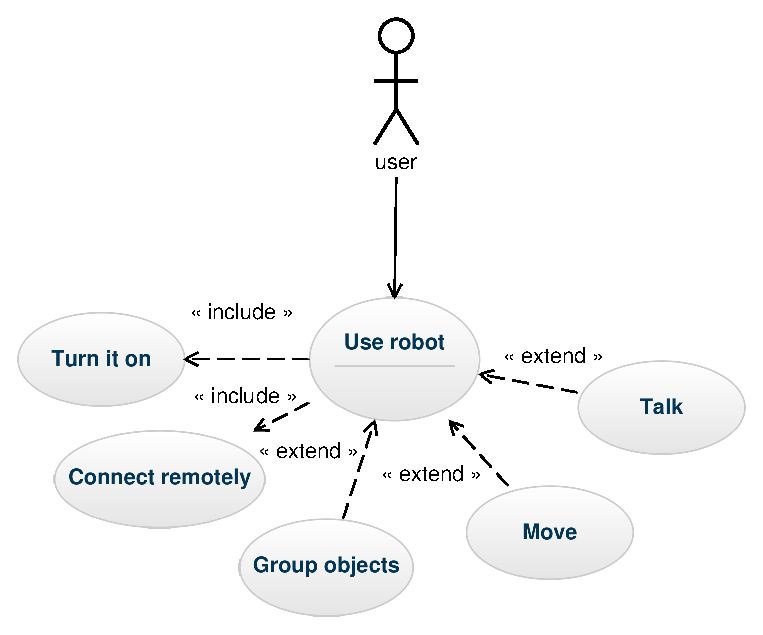
\includegraphics[width=0.45\linewidth]{useCase1.eps}
         }
        \hfil 
        \subfloat[ Group objects use case]
         {
          \label{useCase2}
          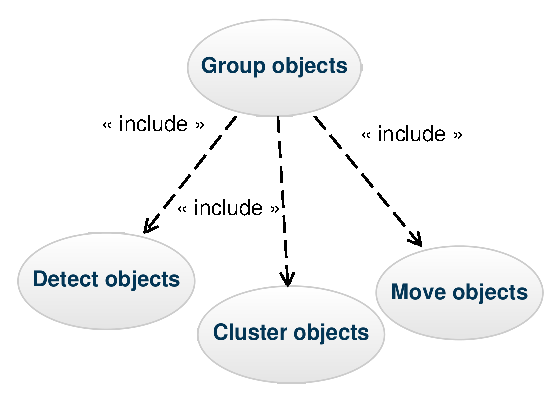
\includegraphics[width=0.45\linewidth]{useCase2.eps} 
         }
         \renewcommand\thefigure{B.1}
        \caption{ Use cases I}
        \label{useCases1}
      \end{figure}

            \begin{figure}[h!]
        \centering
        \subfloat[ Detect objects use case]
         {
         \label{useCase3}
          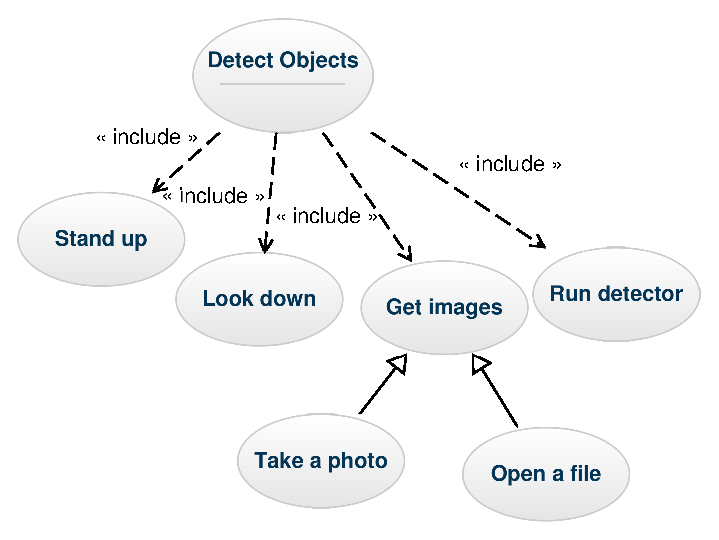
\includegraphics[width=0.45\linewidth]{useCase3.eps}
         }
        \hfil 
        \subfloat[ Move objects use case]
         {
          \label{useCase3}
          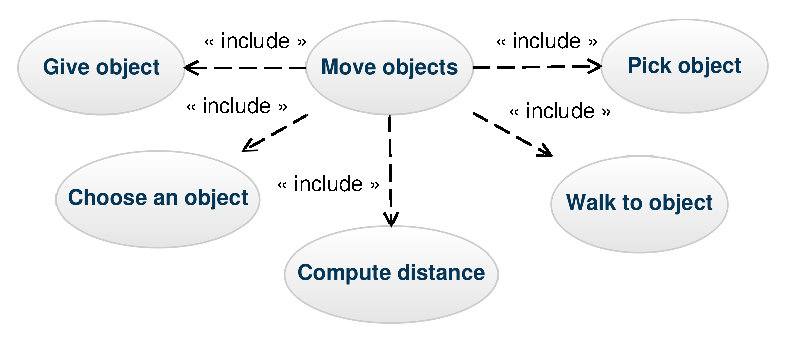
\includegraphics[width=0.45\linewidth]{useCase4.eps} 
         }
         \renewcommand\thefigure{B.2}
        \caption{ Use cases II}
        \label{useCases2}
      \end{figure}

% \begin{figure}[!ht]
% \renewcommand\thefigure{A.1}
% \centering
% 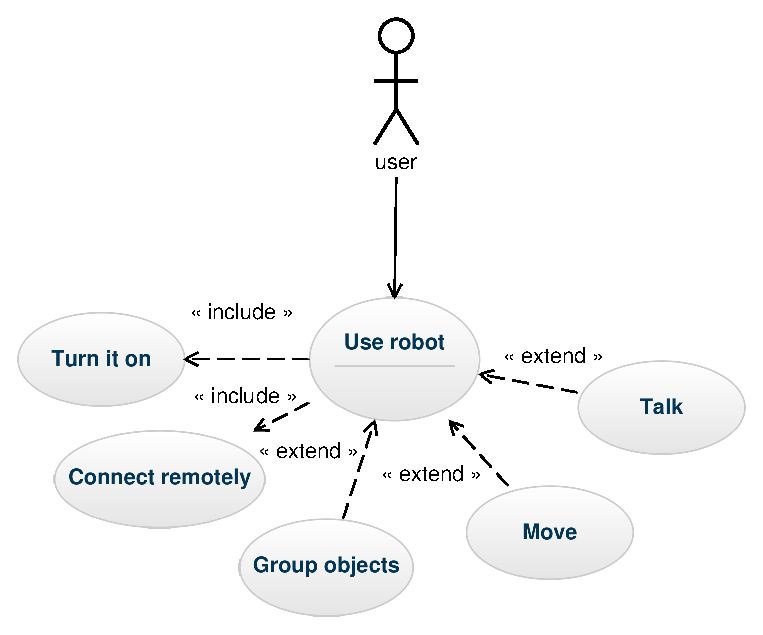
\includegraphics[scale=0.8]{useCase1.eps}
% \caption{Robot's use case}\label{useCase1}
% \end{figure}

% \begin{figure}[!hb]
% \renewcommand\thefigure{A.2}
% \centering
% 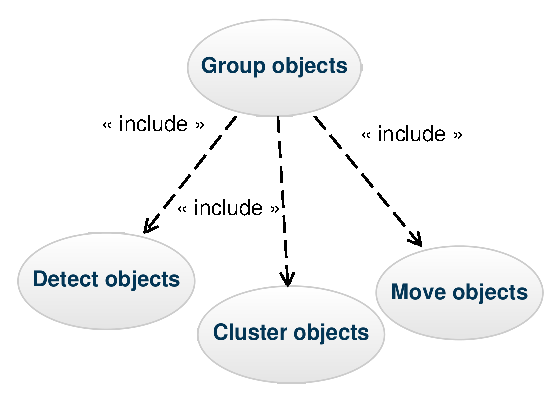
\includegraphics[scale=0.8]{useCase2.eps}
% \caption{Group objects use case}\label{useCase2}
% \end{figure}

% \begin{figure}[!ht]
% \renewcommand\thefigure{A.3}
% \centering
% 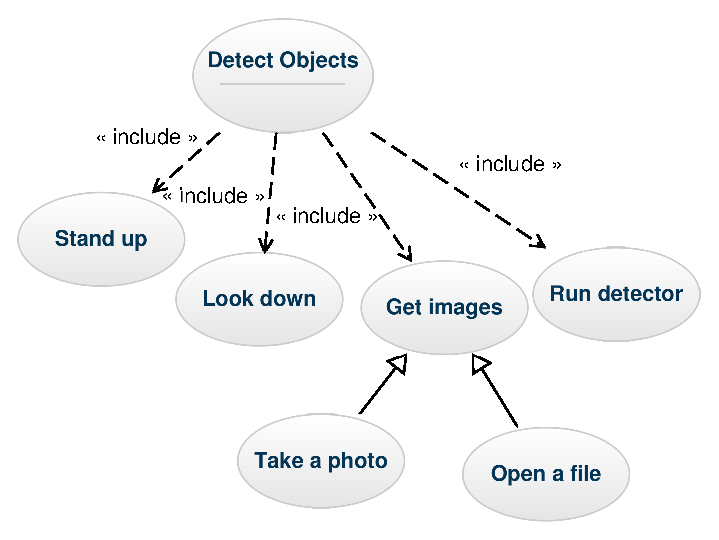
\includegraphics[scale=0.8]{useCase3.eps}
% \caption{Detect objects use case}\label{useCase3}
% \end{figure}

% \begin{figure}[!hb]
% \renewcommand\thefigure{A.4}
% \centering
% 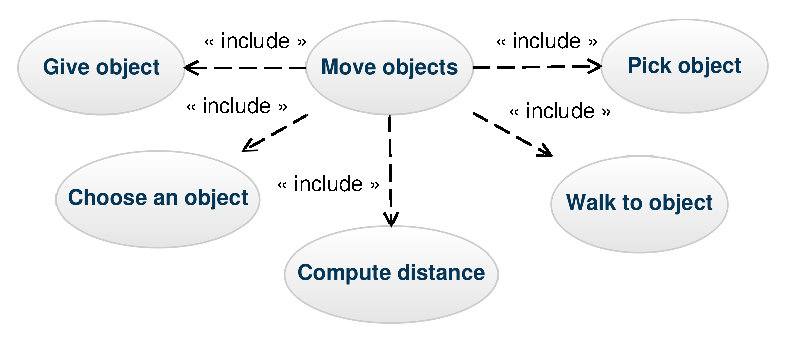
\includegraphics[scale=0.8]{useCase4.eps}
% \caption{Move objects use case}\label{useCase4}
% \end{figure}

\begin{figure}[!ht]
\renewcommand\thefigure{B.3}
\centering
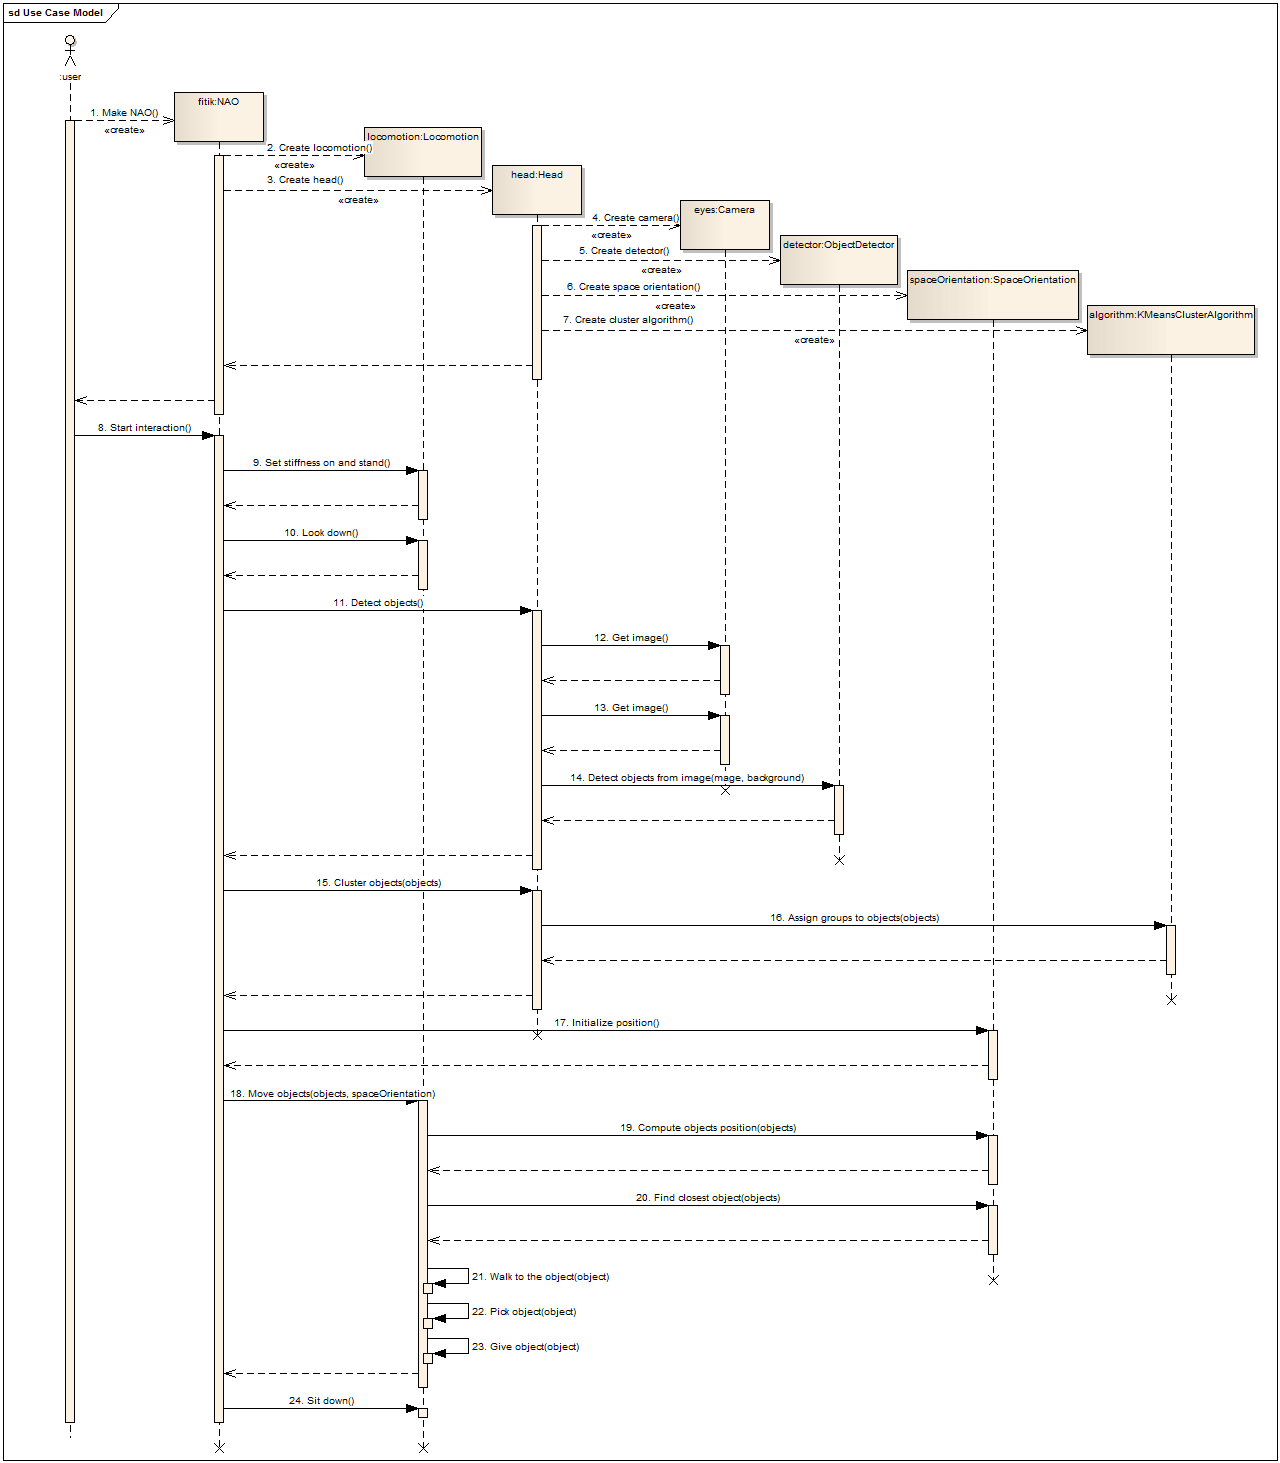
\includegraphics[width=\linewidth]{sequence.png}
\caption{A model of interaction between objects}\label{sequence}
\end{figure}

\begin{figure}[!hb]
\renewcommand\thefigure{B.4}
\centering
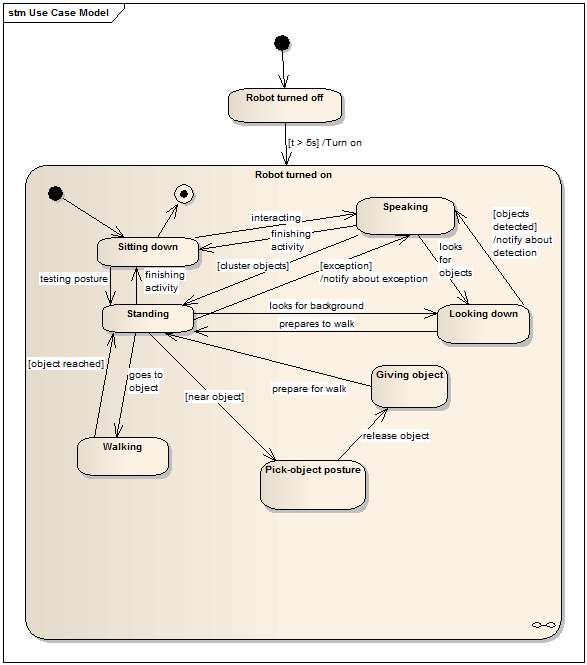
\includegraphics[scale=1]{state.png}
\caption{Robot's states}\label{state}
\end{figure}

\begin{figure}[!ht]
\renewcommand\thefigure{B.5}
\centering
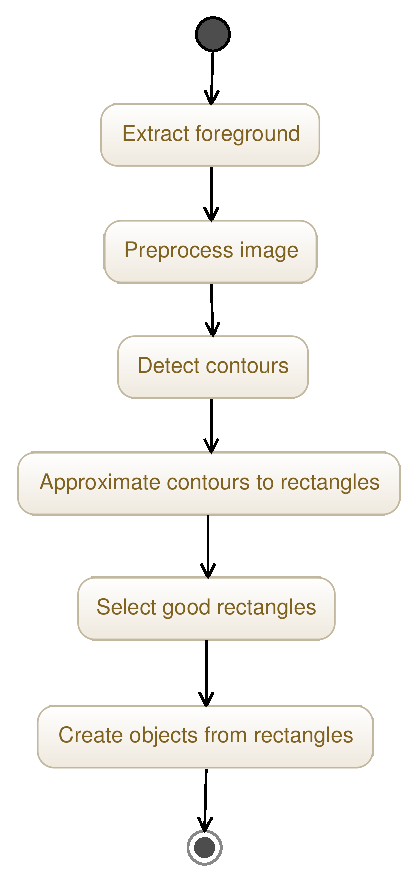
\includegraphics[scale=0.9]{activityObjectDetection.eps}
\caption{Object detection algorithm's steps}\label{activity1}
\end{figure}

\begin{figure}[!hb]
\renewcommand\thefigure{B.6}
\centering
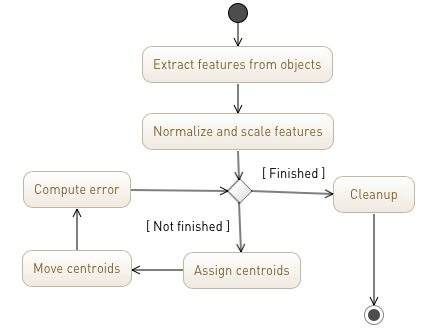
\includegraphics[scale=0.7]{activityCluster.png}
\caption{Clustering algorithm's steps}\label{activity2}
\end{figure}



\clearpage

\section*{Appendix B. Source Code}
\phantomsection
% \renewcommand\thelisting{A.1}
	\lstinputlisting[language=C++, title={SpaceOrientation class interface}, label=list21]{../SrcCode/SpaceOrientation.h}

	\lstinputlisting[language=C++, title={SpaceOrientation class implementation}, label=list22]{../SrcCode/SpaceOrientation.cpp}

	\lstinputlisting[language=C++, title={Head class interface}, label=list23]{../SrcCode/Head.h}

	\lstinputlisting[language=C++, title={Head class implementation}, label=list24]{../SrcCode/Head.cpp}

	\lstinputlisting[language=C++, title={NAO class interface}, label=list25]{../SrcCode/NAO.h}

	\lstinputlisting[language=C++, title={NAO class implementation}, label=list26]{../SrcCode/NAO.cpp}

	\lstinputlisting[language=C++, title={Main file}, label=list27]{../SrcCode/main.cpp}

% 	% \lstinputlisting[language=C++, title={Image class interface}, caption={Source code}, label=list4]{../SrcCode/Image.h}

% 	% \lstinputlisting[language=C++, title={Image class implementation}, label=list4]{../SrcCode/Image.cpp}

% 	% \lstinputlisting[language=C++, title={AbstractImageFetcher class interface}, label=list4]{../SrcCode/AbstractImageFetcher.h}

% 	% \lstinputlisting[language=C++, title={AbstractImageFetcher class implementation}, label=list4]{../SrcCode/AbstractImageFetcher.cpp}

% 	% \lstinputlisting[language=C++, title={ImageFetcherOnOSX class interface}, label=list4]{../SrcCode/ImageFetcherOnOSX.h}

% 	% \lstinputlisting[language=C++, title={ImageFetcherOnOSX class implementation}, label=list4]{../SrcCode/ImageFetcherOnOSX.cpp}

% 	% \lstinputlisting[language=C++, title={Camera class interface}, label=list4]{../SrcCode/Camera.h}

% 	% \lstinputlisting[language=C++, title={Camera class implementation}, label=list4]{../SrcCode/Camera.cpp}		

% 	% \lstinputlisting[language=C++, title={Object class interface}, label=list4]{../SrcCode/Object.h}

% 	% \lstinputlisting[language=C++, title={Object class implementation}, label=list4]{../SrcCode/Object.cpp}		

% 	% \lstinputlisting[language=C++, title={ObjectDetector class interface}, label=list4]{../SrcCode/ObjectDetector.h}

% 	% \lstinputlisting[language=C++, title={ObjectDetector class implementation}, label=list4]{../SrcCode/ObjectDetector.cpp}

% 	% \lstinputlisting[language=C++, title={AbstractClusterAlgorithm class interface}, label=list4]{../SrcCode/AbstractClusterAlgorithm.h}

% 	% \lstinputlisting[language=C++, title={AbstractClusterAlgorithm class implementation}, label=list4]{../SrcCode/AbstractClusterAlgorithm.cpp}

% 	% \lstinputlisting[language=C++, title={ObjectDetector class interface}, label=list4]{../SrcCode/ObjectDetector.h}

% 	% \lstinputlisting[language=C++, title={ObjectDetector class implementation}, label=list4]{../SrcCode/ObjectDetector.cpp}

% 	% \lstinputlisting[language=C++, title={KMeansClusteringAlgorithm class interface}, label=list4]{../SrcCode/KMeansClusteringAlgorithm.h}

% 	% \lstinputlisting[language=C++, title={KMeansClusteringAlgorithm class implementation}, label=list4]{../SrcCode/KMeansClusteringAlgorithm.cpp}

% 	% \lstinputlisting[language=C++, title={Speech class interface}, label=list4]{../SrcCode/Speech.h}

% 	% \lstinputlisting[language=C++, title={Speech class implementation}, label=list4]{../SrcCode/SpeechBig.cpp}

% 	% \lstinputlisting[language=C++, title={Head class interface}, label=list4]{../SrcCode/Head.h}

% 	% \lstinputlisting[language=C++, title={Head class implementation}, label=list4]{../SrcCode/Head.cpp}

% 	% \lstinputlisting[language=C++, title={CustomMoves class interface}, label=list4]{../SrcCode/CustomMoves.h}

% 	% \lstinputlisting[language=C++, title={CustomMoves class implementation}, label=list4]{../SrcCode/CustomMoves.cpp}

% 	% \lstinputlisting[language=C++, title={Locomotion class interface}, label=list4]{../SrcCode/Locomotion.h}

% 	% \lstinputlisting[language=C++, title={Locomotion class implementation}, label=list4]{../SrcCode/Locomotion.cpp}

% 	% \lstinputlisting[language=C++, title={SpaceOrientation class interface}, label=list4]{../SrcCode/SpaceOrientation.h}

% 	% \lstinputlisting[language=C++, title={SpaceOrientation class implementation}, label=list4]{../SrcCode/SpaceOrientation.cpp}




	






\clearpage




\cleardoublepage
 
 
\end{document}